\documentclass[11pt, spanish]{article}
\usepackage[spanish]{babel}
\selectlanguage{spanish}
\usepackage[utf8]{inputenc}
\usepackage{graphicx}
\usepackage{mathtools}
\usepackage{tabularx}
\usepackage[font=small,labelfont=bf]{caption}
\usepackage{subcaption}
\usepackage{authblk}

\captionsetup[table]{name=Tabla}
\renewcommand{\thetable}{\Roman{figure}}
\newcommand{\mean}[1]{\left\langle#1\right\rangle}
%\newcommand{\eqref}[1]{Ec.~\ref{#1}}

\begin{document}
\begin{titlepage}
    \centering
    {\scshape\LARGE Universidad de Buenos Aires \par}
    \vspace{1cm}
    {\scshape\Large Informe 1\par}
    \vspace{1.5cm}
    {\huge\bfseries Redes Complejas\par}
    \vspace{2cm}
    {\Large\itshape Ra\'ul Barriga\par}
    {\Large\itshape Mariela Celis\par}
    {\Large\itshape Jimmy Mas\'ias\par}
    {\Large\itshape Sebast\'ian Pinto\par}

    \vfill

    \vfill

                                                    % Bottom of the page
    {\large \today\par}
\end{titlepage}
    %\input{intro}


\section{Ejercicio 1}

Se consideran tres redes de interacci\'on prote\'inas de levadura \textit{Saccharomyces cerevisiae}: 
La red de complejos proteicos (red AP-MS) relaciona las proteinas que, formando un complejo proteico
(estructura cuaternaria), generan una estructura medible a trav\'es de \textit{Mass Spectrometry} 
(esta tecnica es conocida como \textit{Affinity Purification/Mass Spectrometry}  \citep{apms_data}; 
La red de interacciones Binarias obtenida a trav\'es de la t\'ecnica \textit{yeast 2 hybrid} 
(Y2H) \citep{y2h_data}; y la red de interacciones reportadas en la literatura \citep{lit_data}.
Todas estas redes est\'an disponibles en \textit{Yeast Interactome Database}
\footnote{interactome.dfci.harvard.edui/S\_cerevisiae/}, y son 
mostradas en la figura \ref{fig:ej1_grafos}.

% La idea del ejercicio es realizar un analisis cuantitativo de las tres redes
% y observar las coherencia entre las interacciones reportadas


\begin{figure}[!ht]
    \centering
    \begin{subfigure}[b]{0.30\columnwidth}
        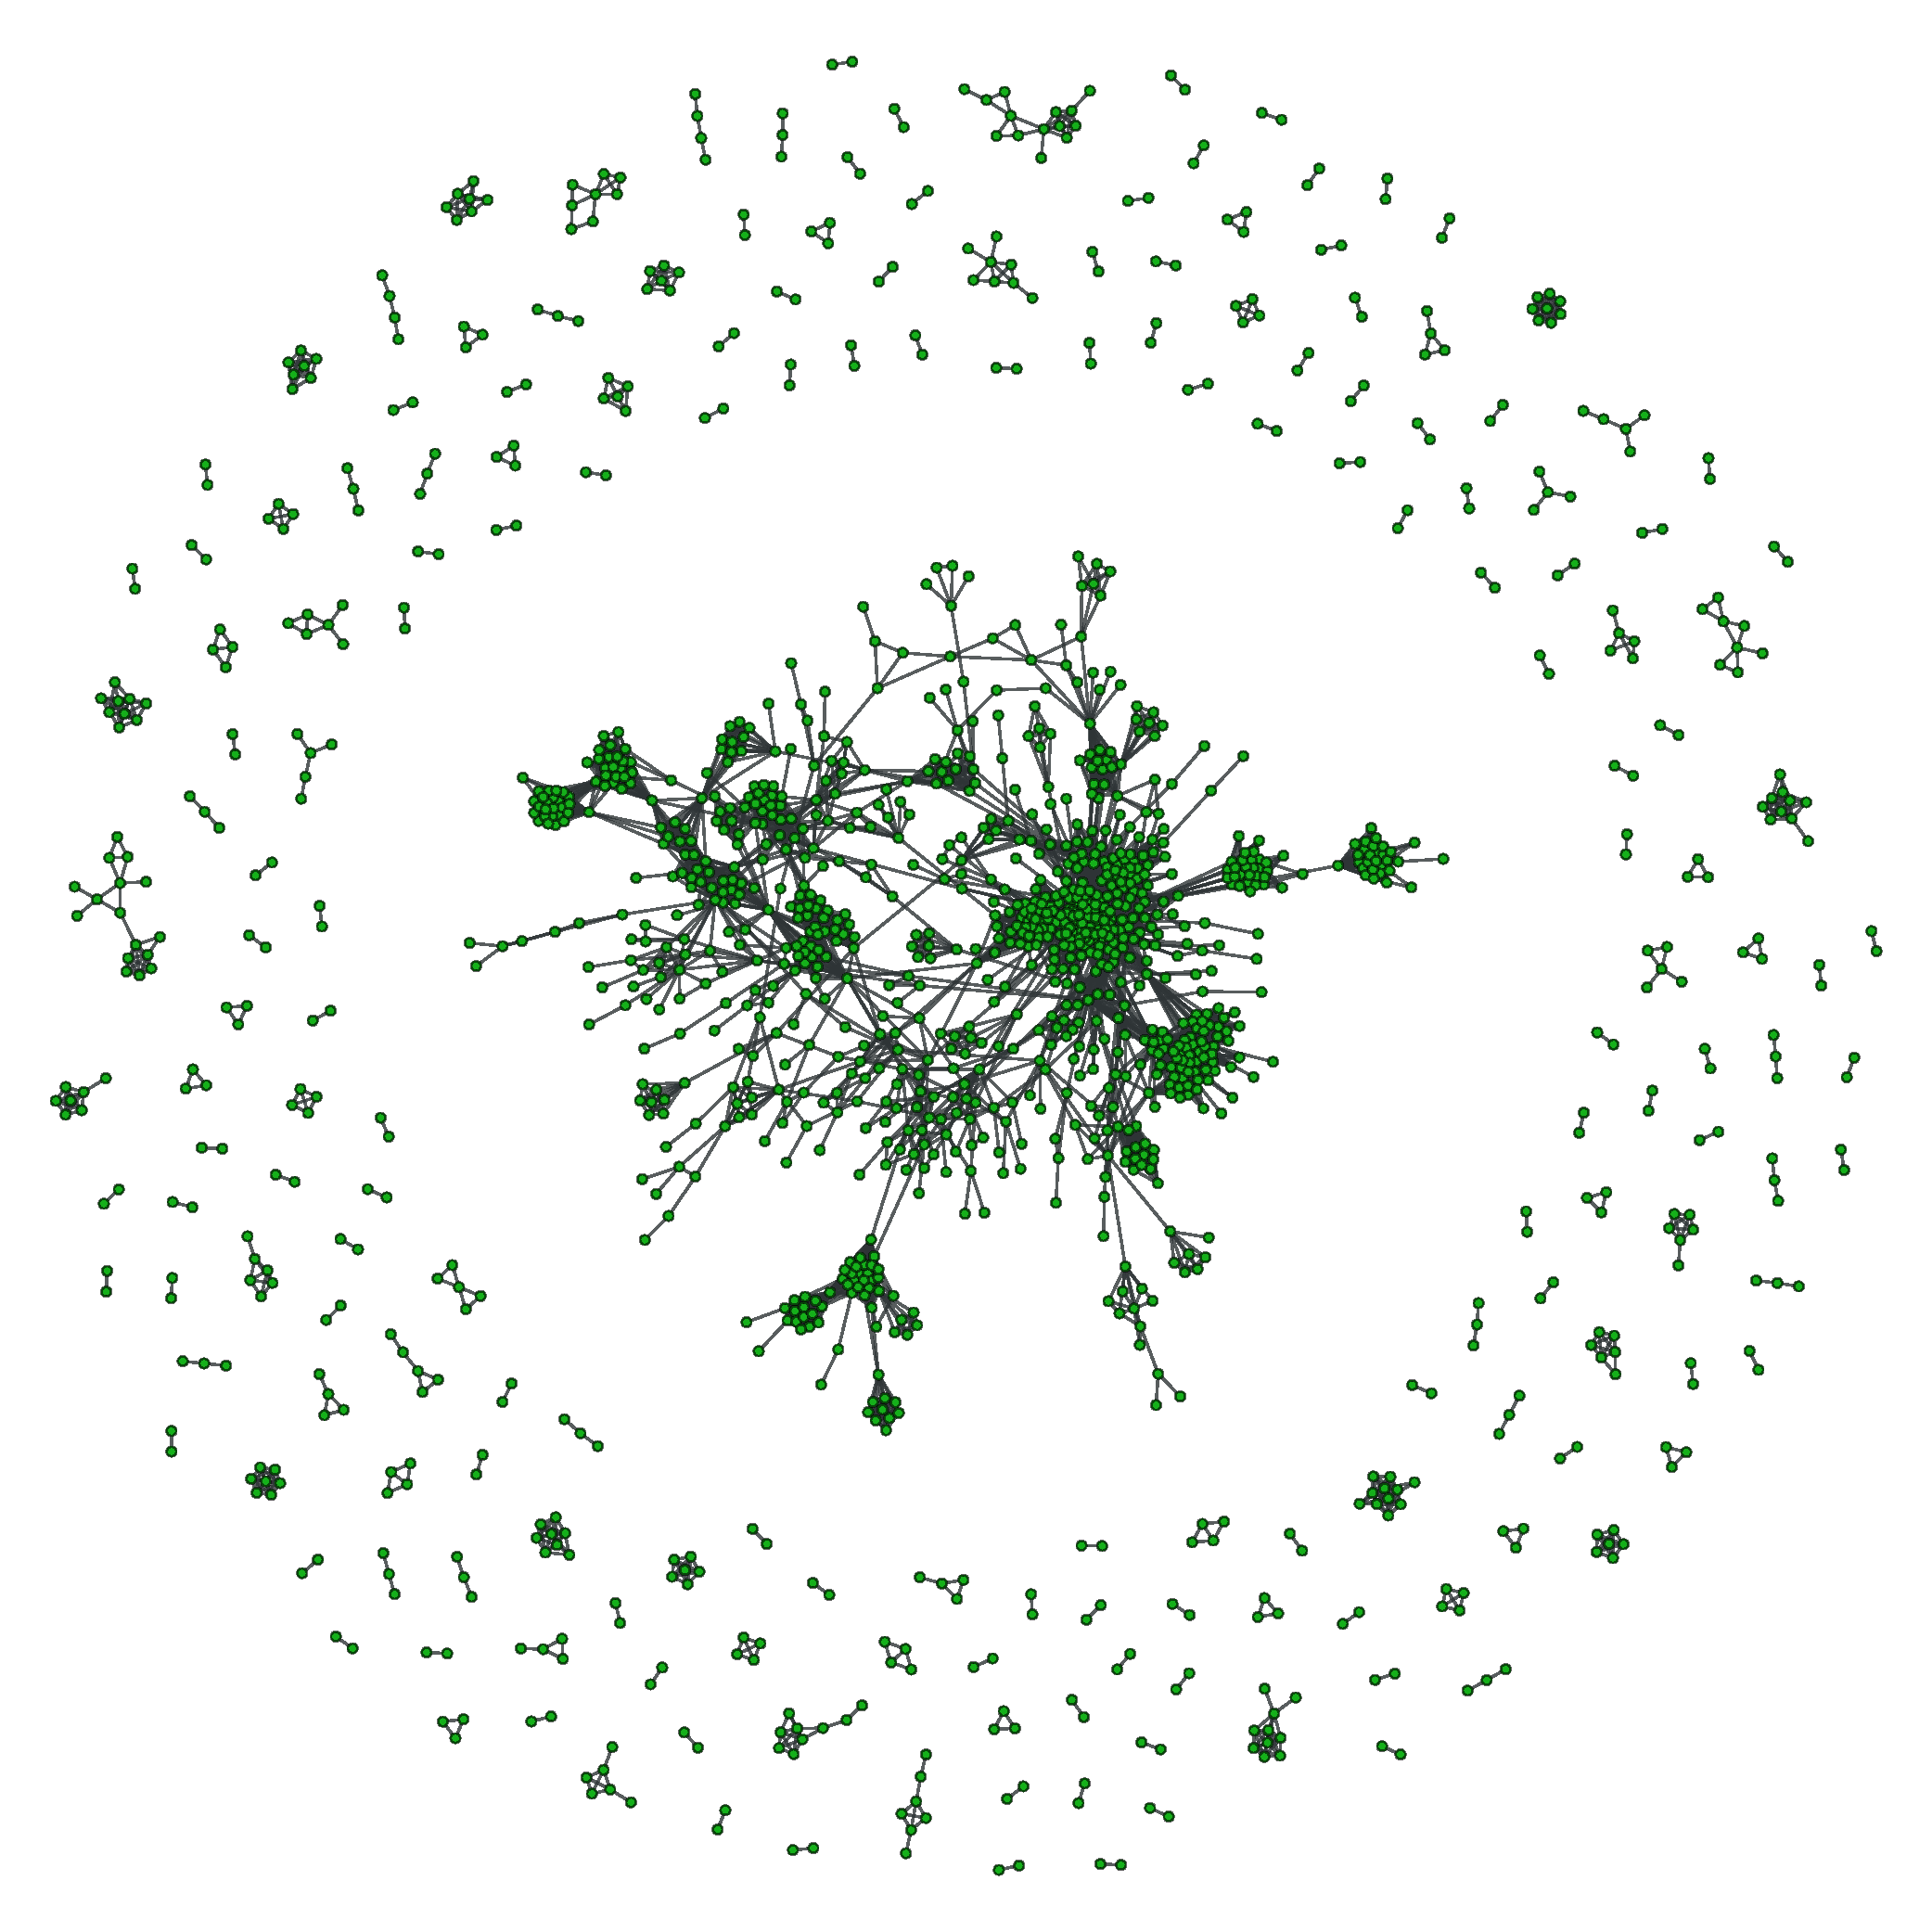
\includegraphics[width=\textwidth]{./schemes/yeast_AP-MS-txt.pdf}
        \caption{\label{fig:ap_ms} AP-MS}
    \end{subfigure}
    \begin{subfigure}[b]{0.30\columnwidth}
        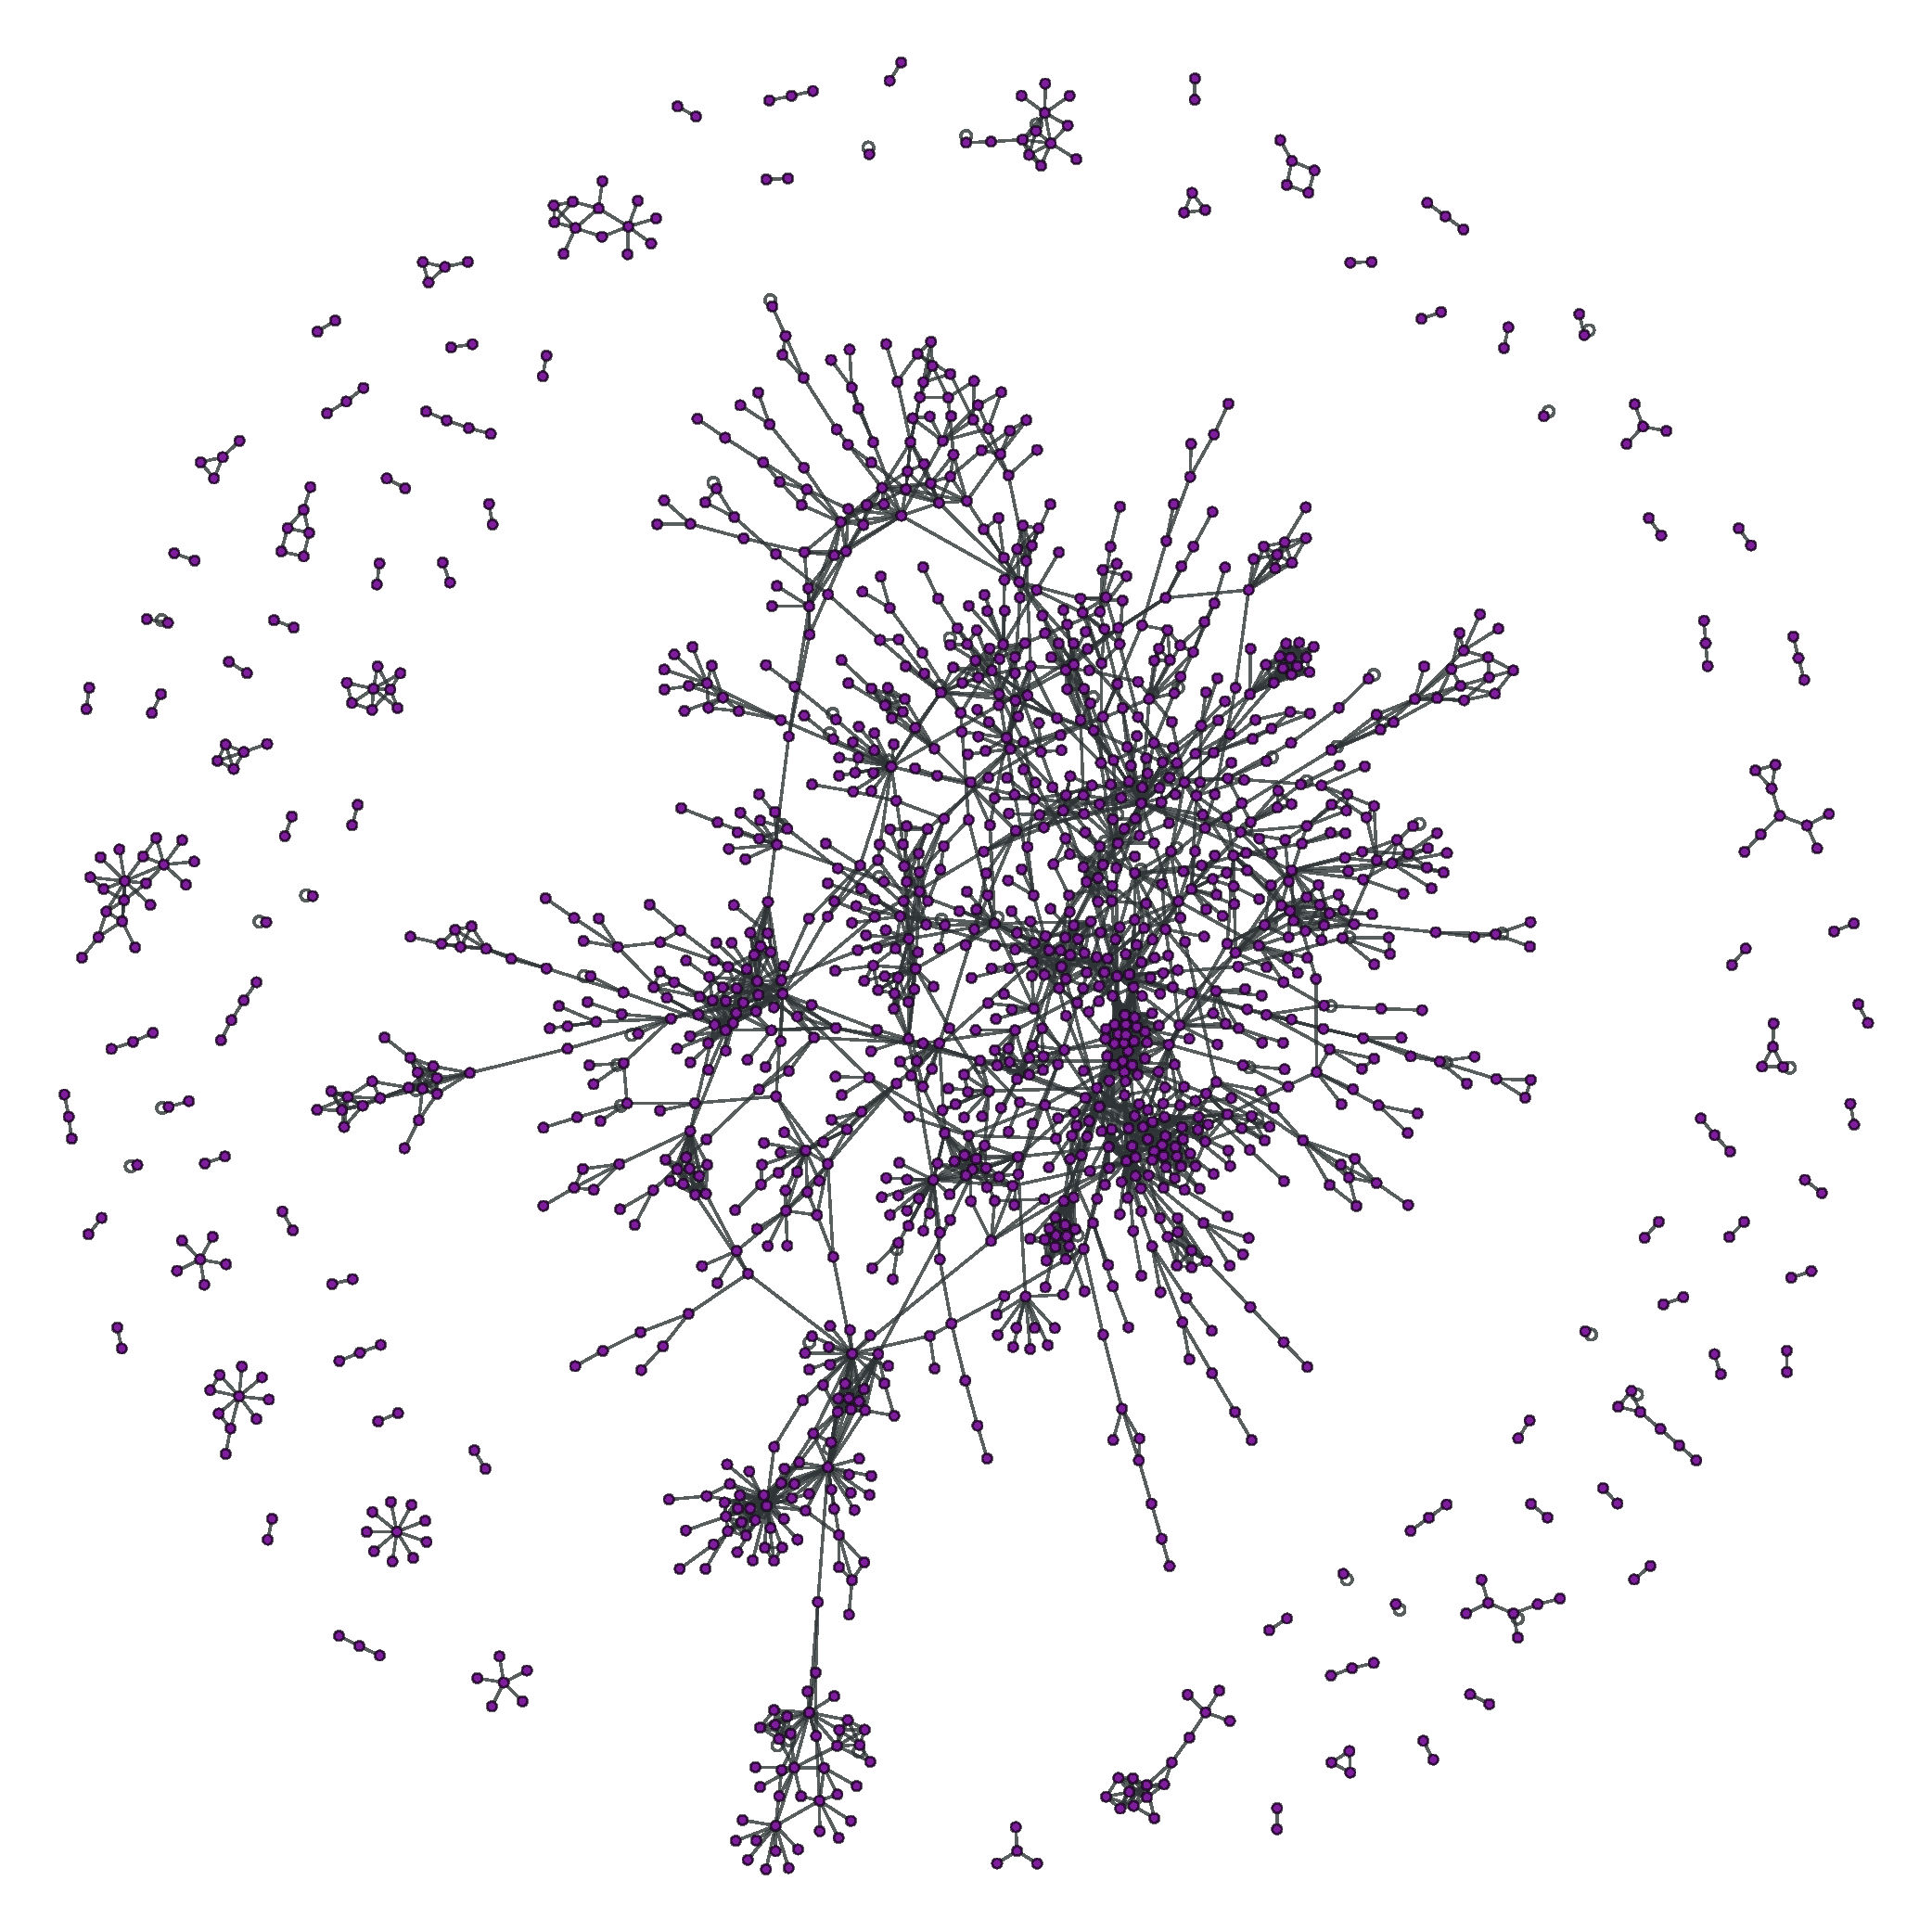
\includegraphics[width=\textwidth]{./schemes/yeast_LIT-txt.pdf}
        \caption{\label{fig:LIT}LIT}
    \end{subfigure}
    \begin{subfigure}[b]{0.30\columnwidth}
        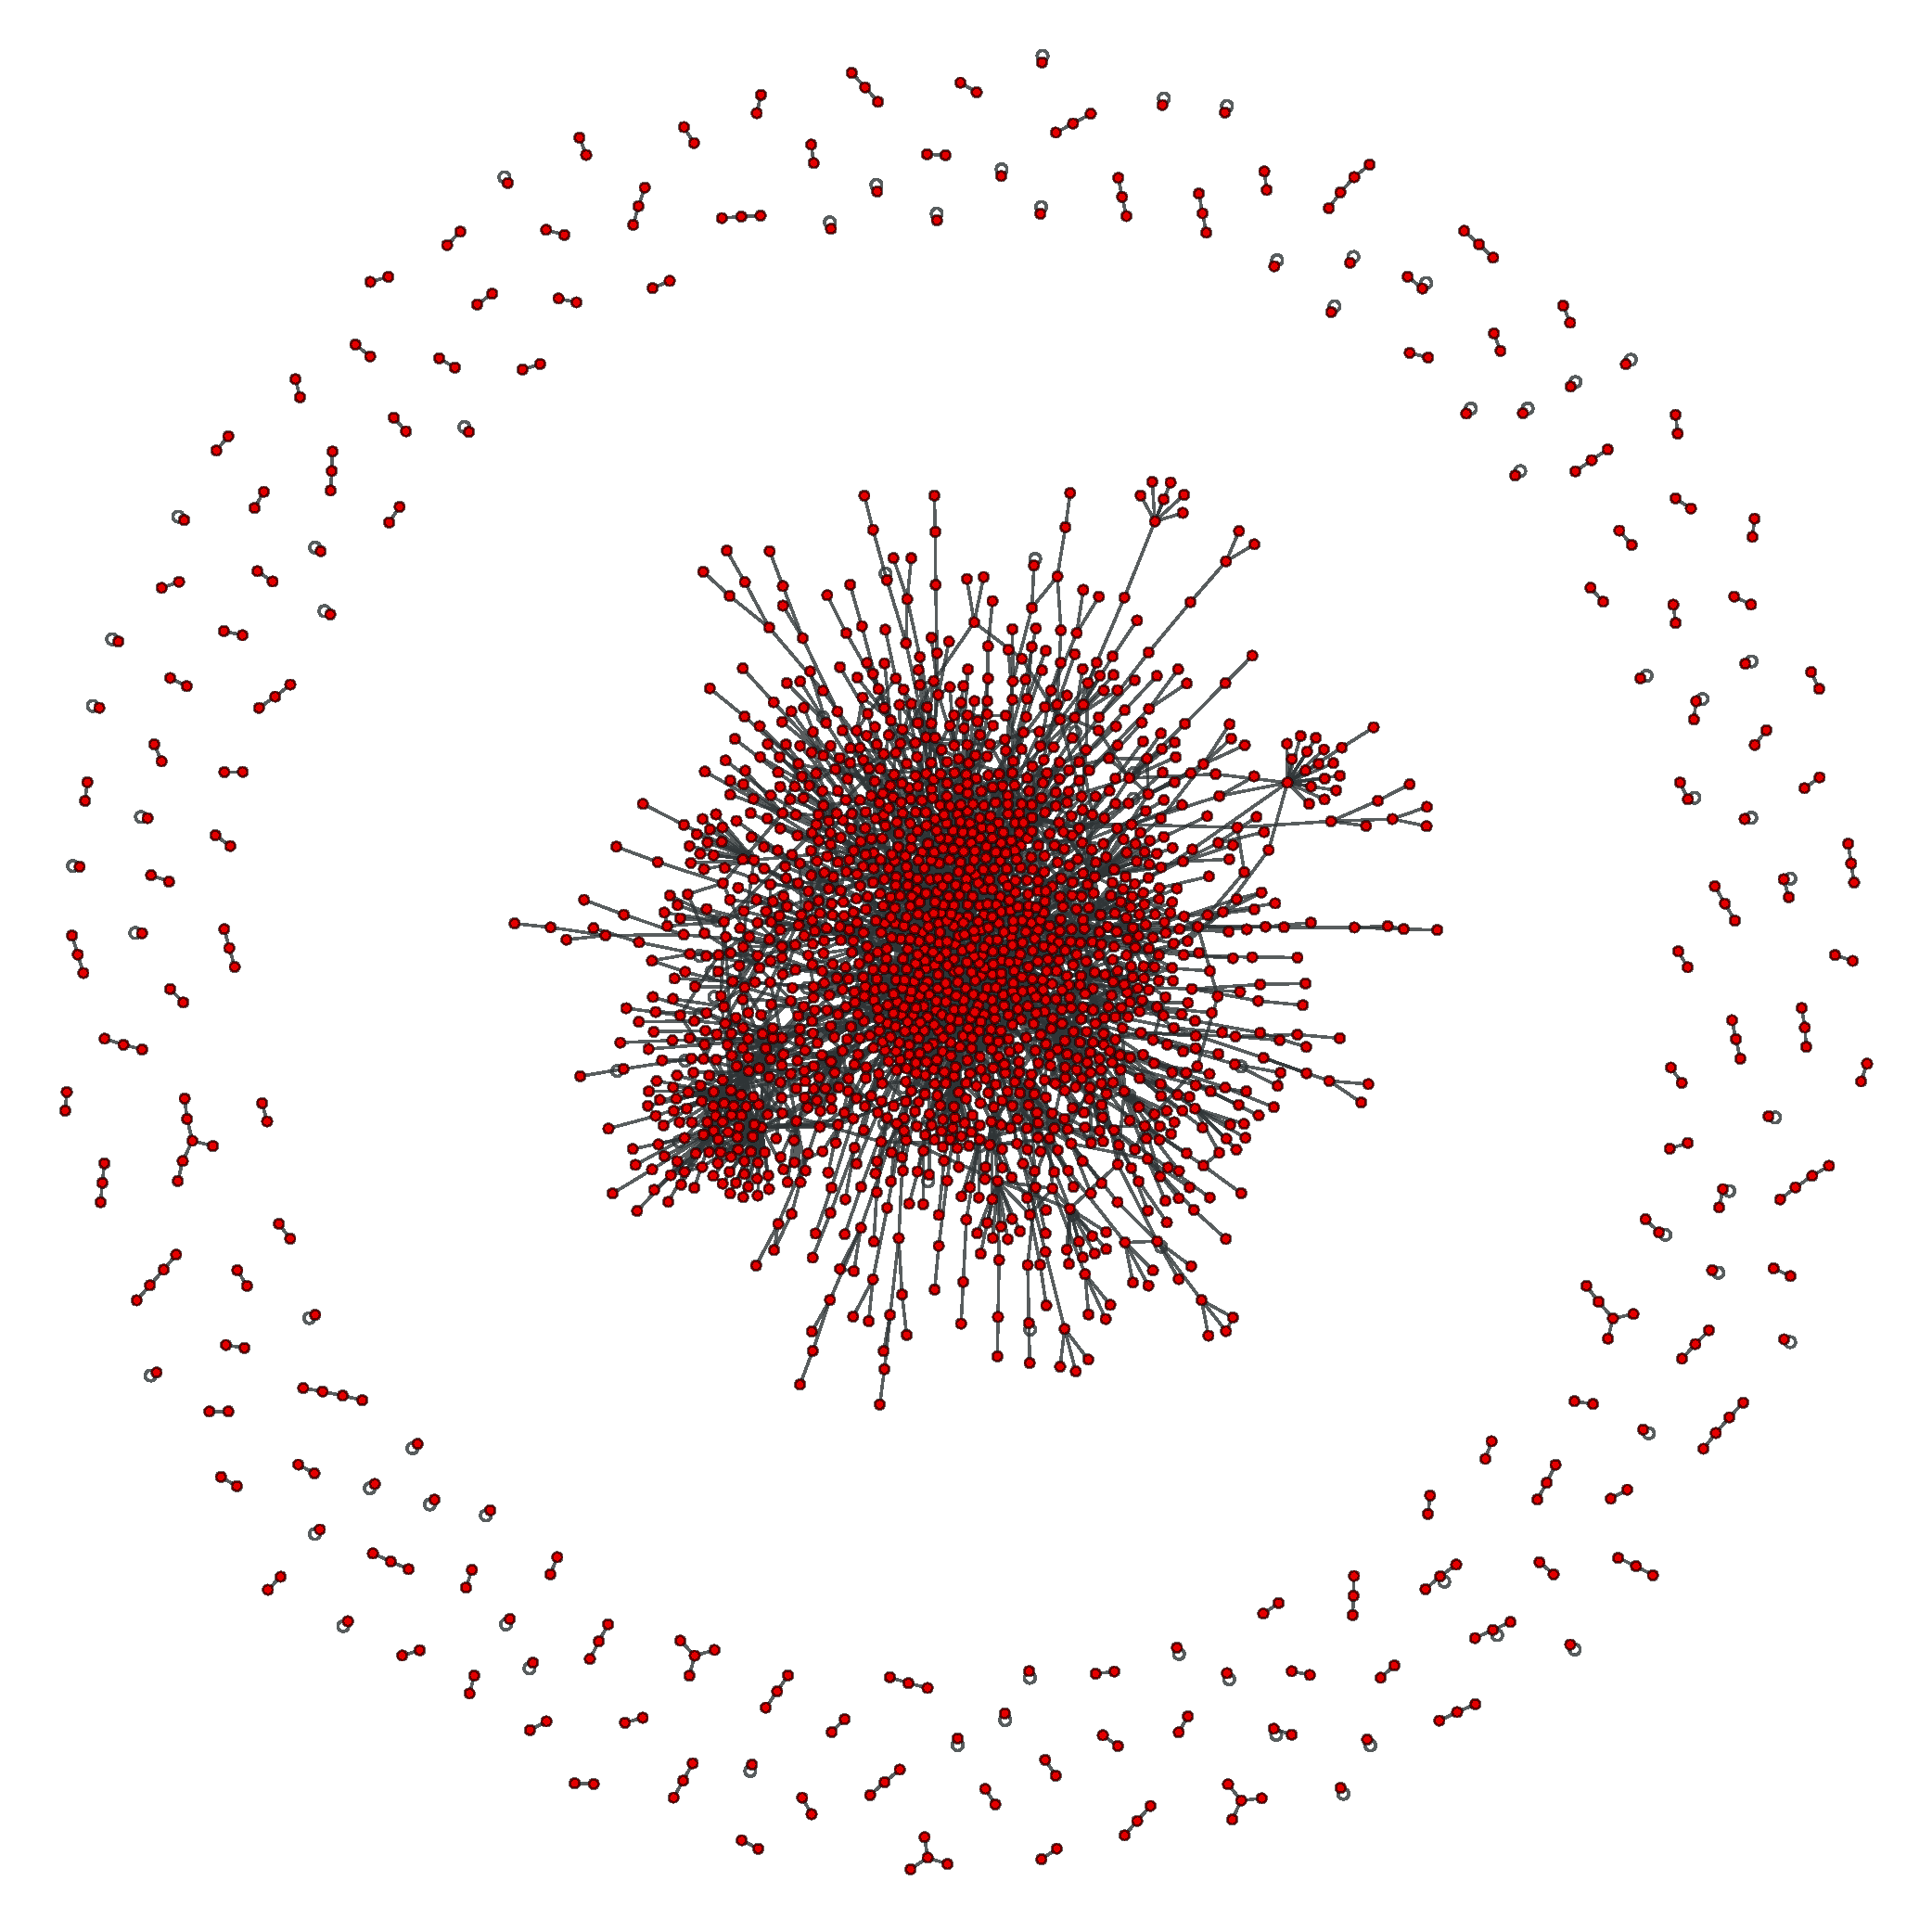
\includegraphics[width=\textwidth]{./schemes/yeast_Y2H-txt.pdf}
        \caption{\label{fig:y2h} Y2H}
    \end{subfigure}
    \caption{\label{fig:ej1_grafos} Esquematizaci\'on de los grafos de cada 
    red estudiada. Se utiliz\'o un \textit{layout} SFDP, de la libreria \texttt{graph-tool},
    y pueden ser reproducidas usando \texttt{plot.py~<archivo>\;\;-f <format>}    }
\end{figure}

\subsection{Caracterizaci\'on de las redes}
Una caracterizacion global y cuantitativa de las redes se muestra en la 
Tabla~\ref{tab:obs}. 



\begin{table}[!ht]
    \centering
    \caption{\label{tab:obs}Observables para las tres redes de interacci\'on prote\'ica de levadura.}
    {\scriptsize
    \begin{tabularx}{1\columnwidth}{XlX|XcXcXcX}
        \hline\hline
        &Observables        &&& AP-MS && LIT && Y2H &\\ 
        \hline
        &N$^o$ nodos $N$    &&& 1622 && 1536 && 2018 &\\
        &N$^o$ enlaces $L$  &&& 9070 && 2925 && 2930 &\\
        &Densidad           &&& 0.0068 && 0.0024 && 0.0014 &\\
        &Diametro           &&& 15 && 19 && 14 &\\
        \hline
        &Grado $k$&&&\\
  %      \hline
        &\quad medio  $\mean{k}$     &&& 11.18 && 3.80 && 2.93 &\\
        &\quad maximo $\max(\{k\})$  &&& 127  && 40   && 91 &\\ 
        &\quad minimo $\min(\{k\})$  &&& 1    && 1    && 1 &\\ 
        \hline
        &Coeficiente de Clusterizaci\'on&&&\\
%        \hline
        &\quad medio/local $\mean{C}$               &&& 0.0710 && 0.4556 && 0.0970 & \\
        &\quad triangular/global $C_\bigtriangleup$ &&& 0.6185 && 0.3461 && 0.0236 & \\
        \hline\hline
    \end{tabularx}
    }
\end{table}
No es de extra\~nar que, a pesar de que estas 3 redes de proteinas 
pertenecen al mismo organismo (\textit{Saccharomyces cerevisiae}),
estas son distintas topol\'ogicamente debido a la manera en que son armadas.
La red AP-MS muestra la formaci\'on de varios grupos/clusters muy densos que corresponden
a los complejos proteicos purificados, esto se ve reflejado en los observables de la tabla \ref{tab:obs}
en que, salvo el di\'ametro, presenta mayores valores que el resto de las redes. 
Cabe observar que la red de literatura LIT presenta el mayor di\'ametro, sin embargo es la con 
menor grado m\'aximo (por lo que pareciera capaz de relacionar m\'as interacciones entre clusters), debido a la compilaci\'on
de un gran n\'umero de trabajos, pero tiene menor detalle de las interacciones prote\'ina-prote\'ina, debido
a que en general los trabajos consultados son espec\'ificos y por lo tanto sesgados (hay perdida de informaci\'on las proteinas
menos estudiadas).
En particular al observar la clusterizaci\'on es importante diferenciar la clusterizaci\'on media $\mean{C}$ y la 
clusterizaci\'on triangular $C_\bigtriangleup$. La primera caracteriza la media de la clusterizaci\'on local de cada 
nodo, es por ello que la red LIT prensenta el mayor valor, debido a que, como mencionamos antes, compila
trabajos detallados que dan cuenta de peque\~nos clusters. Tanto la red AP-MS y, a\'un m\'as, la red Y2H diluyen
su clusterizaci\'on debido a un gran n\'umero de \textit{peque\~nas interacciones aisladas}. Por otro lado
el coeficiente $C_\bigtriangleup$ es una medida m\'as global, ya que no pesa interacciones bin\'arias puras.
En este \'ultimo caso AP-MS presenta la mayor clusterizaci\'on, mientras que Y2H la menor.


\subsection{Coherencia entre las redes}

\begin{figure}[!ht]
    \centering
    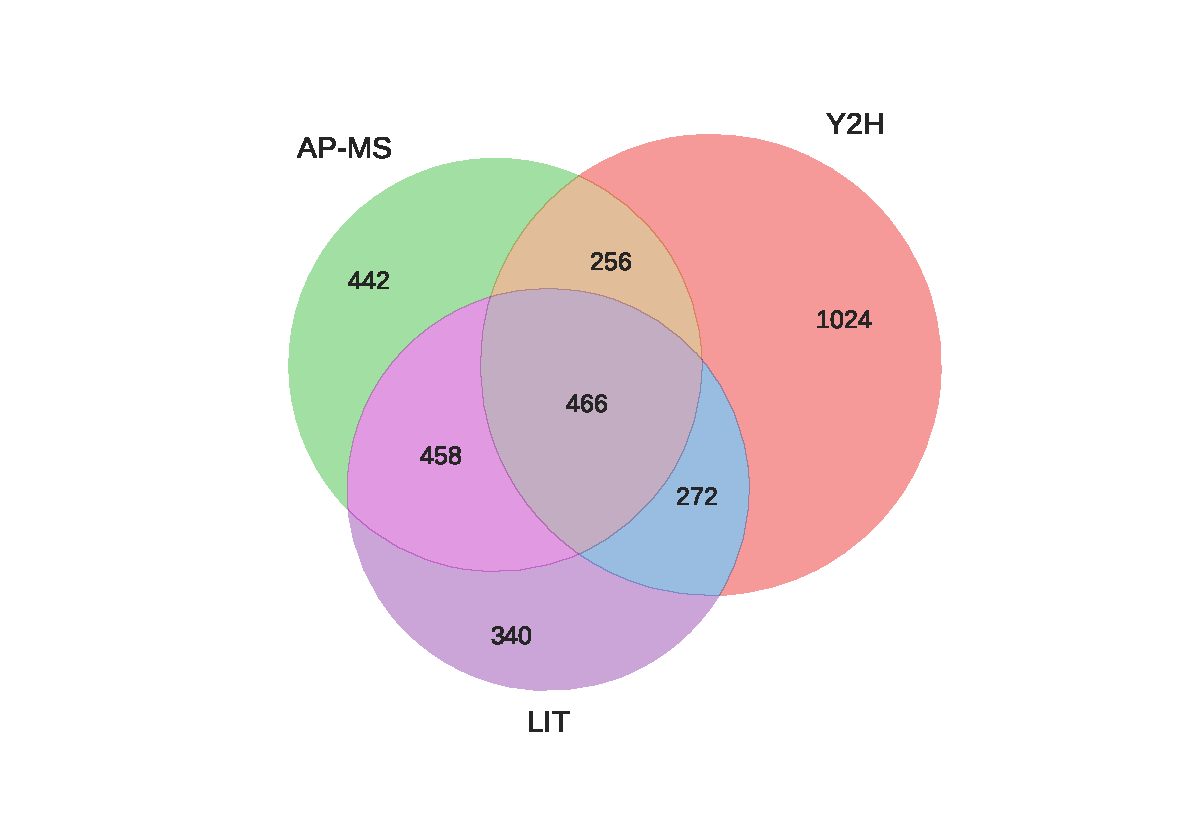
\includegraphics[width=.5\columnwidth]{./schemes/venn_AP-MS-Y2H-LIT_covertura.pdf}
    \caption{\label{fig:cober} Diagrama de Venn para cobertura entre las tres redes. }
\end{figure}



En segundo lugar se analiz\'o la cobertura y coherencia entre las interacci\'ones reportadas
en las redes. Para ello se realiz\'aron los diagramas de Venn mostrados en la figura \ref{fig:cober}, \ref{fig:venn} y \ref{fig:subgrafos}
(estos pueden reproducirse con el script \texttt{venn.py} \texttt{venn2.py}). Para analizar la covertura comparamos
la intersecci\'on de las prote\'inas reportadas en cada caso. En la figura \ref{fig:cober} se muestra
la cobertura de cada red y la cantidad de proteinas reportadas por m\'as de una red (intersecciones). Es 
interesante notar que AP-MS y LIT presentan $\sim 60\%$ de cobertura entre ellas y solo un $\sim 27\%$ 
y un $\sim 22\%$ de las prot\'inas reportadas, respectivamente, son especificas de cada red. Esto se ve contrastado
con el $\sim 50\%$ de especificidad en la red Y2H. 


\vspace{1.5cm}
\begin{figure}[!ht]
    \centering
    \begin{subfigure}[b]{0.48\columnwidth}
        \centering
        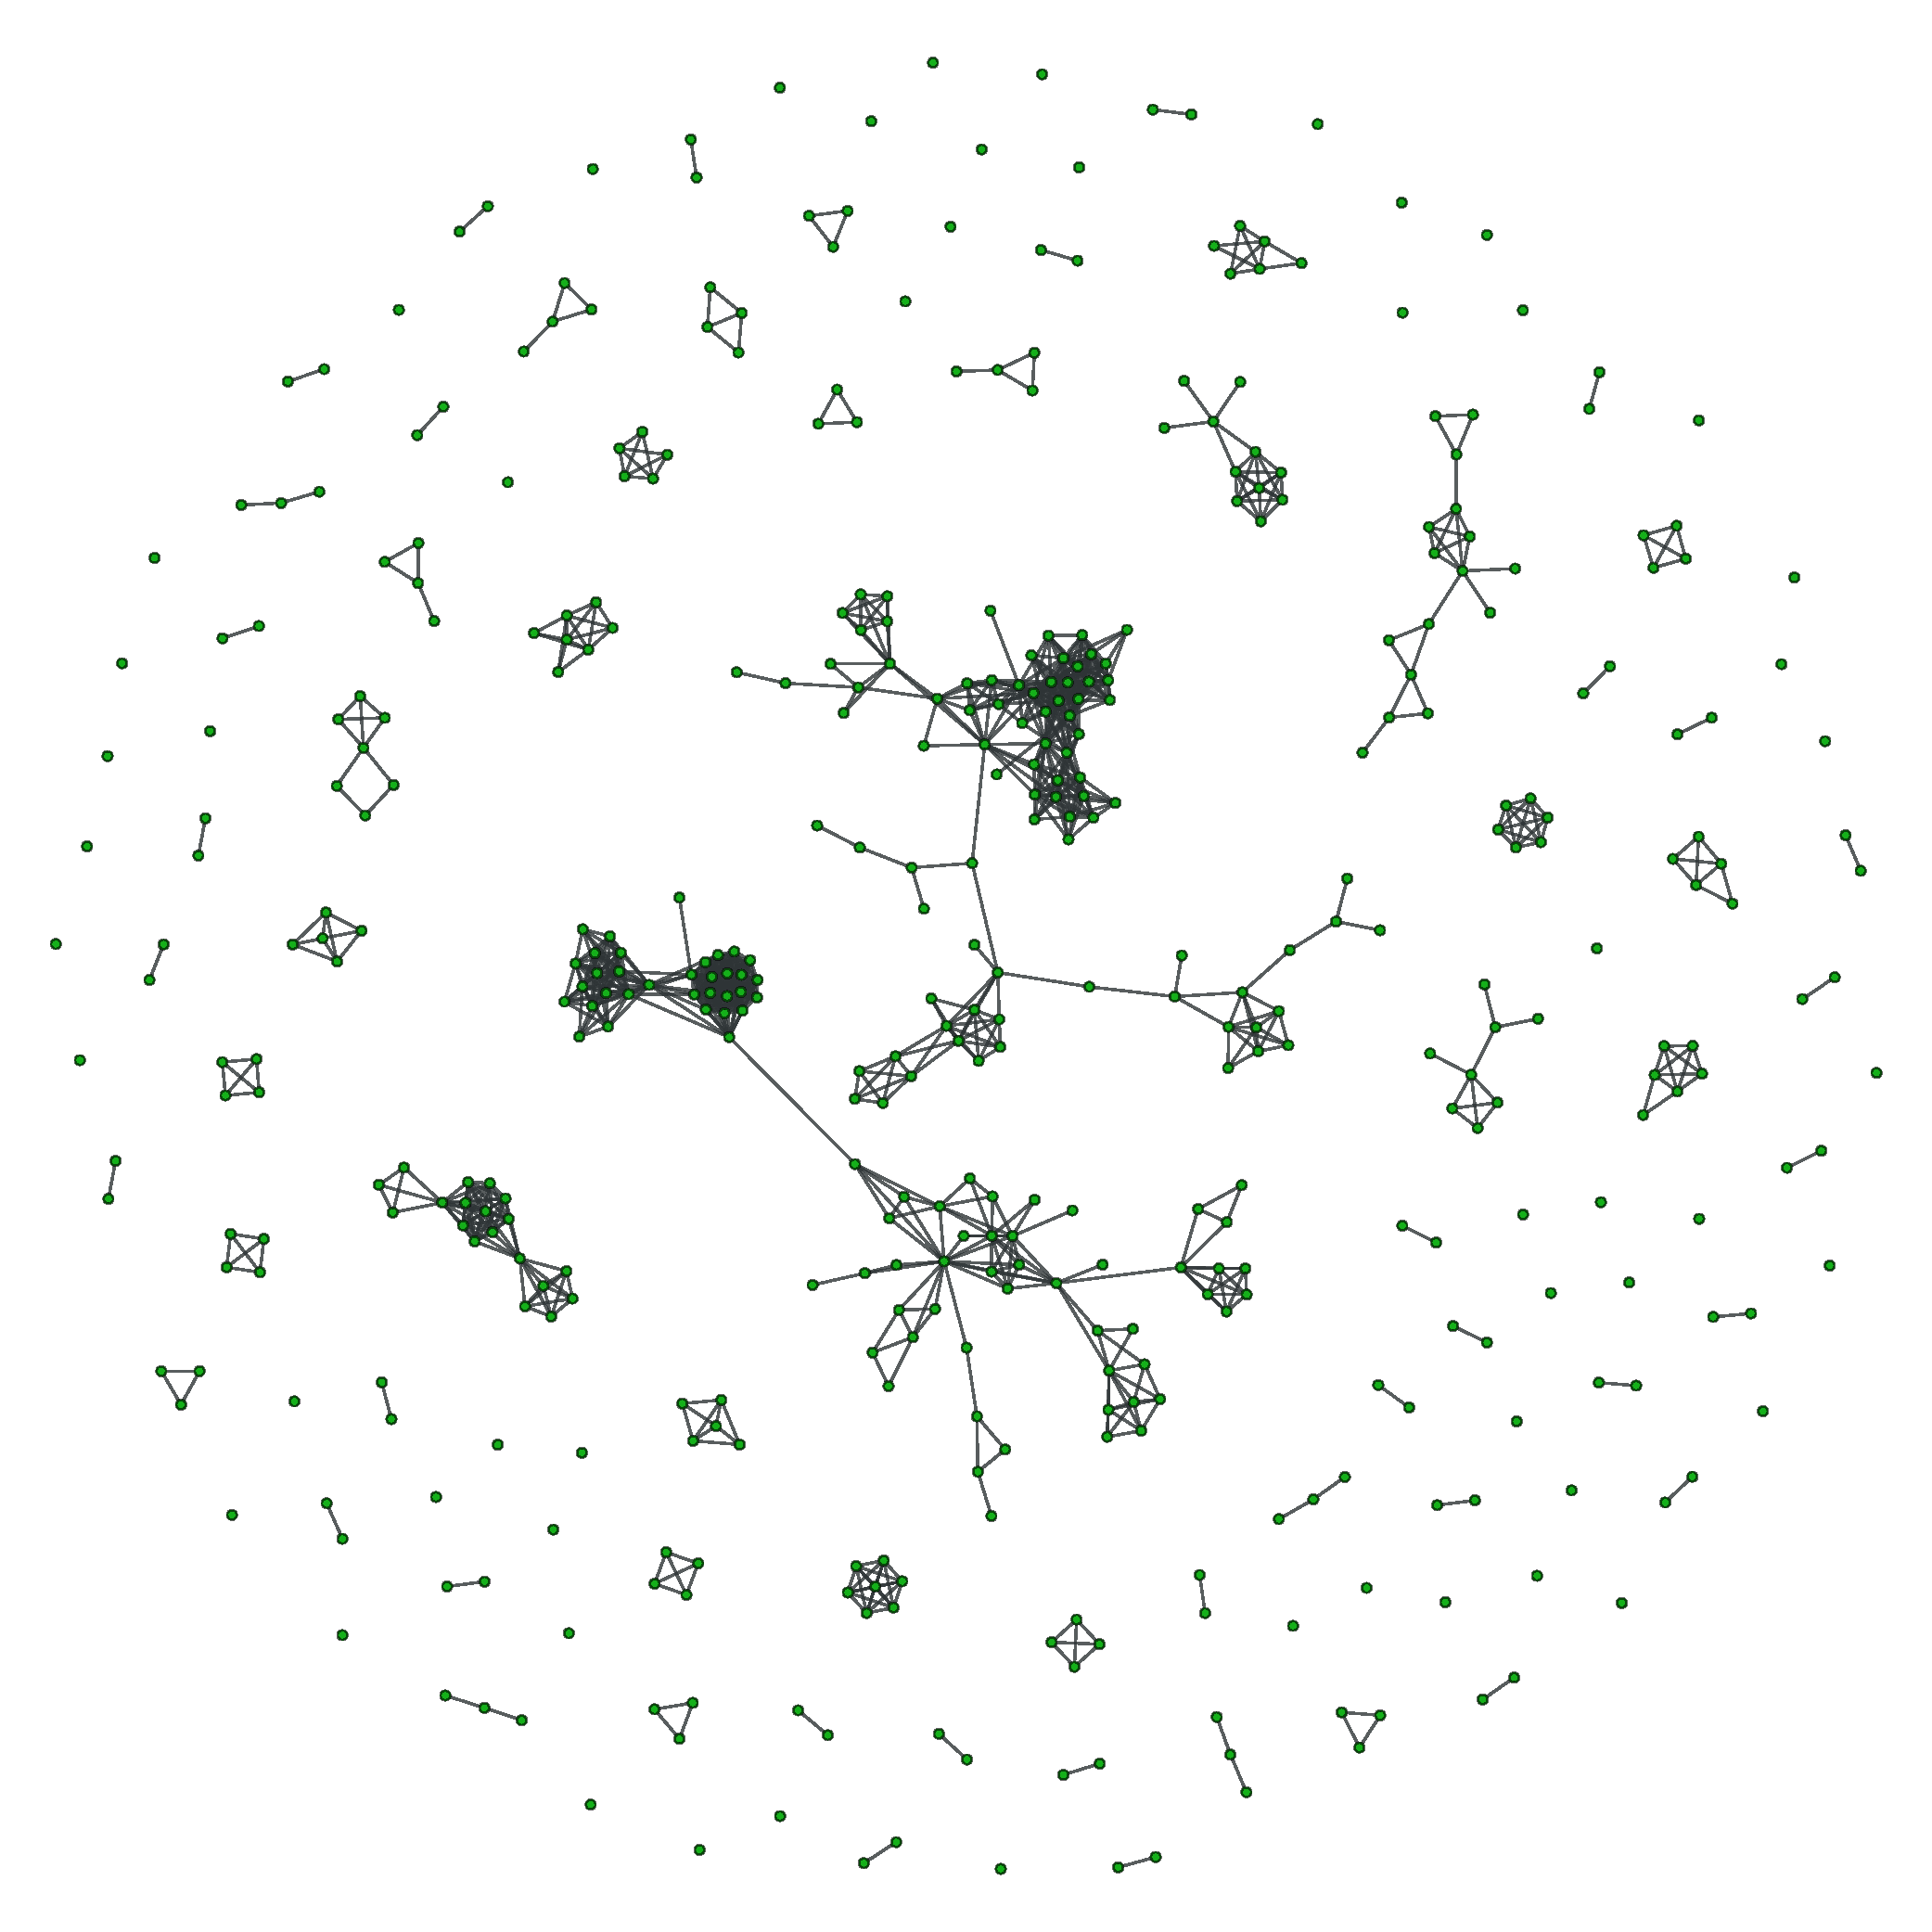
\includegraphics[width=.45\textwidth]{./schemes/subgrafo_AP-MS_all-gml.pdf}
        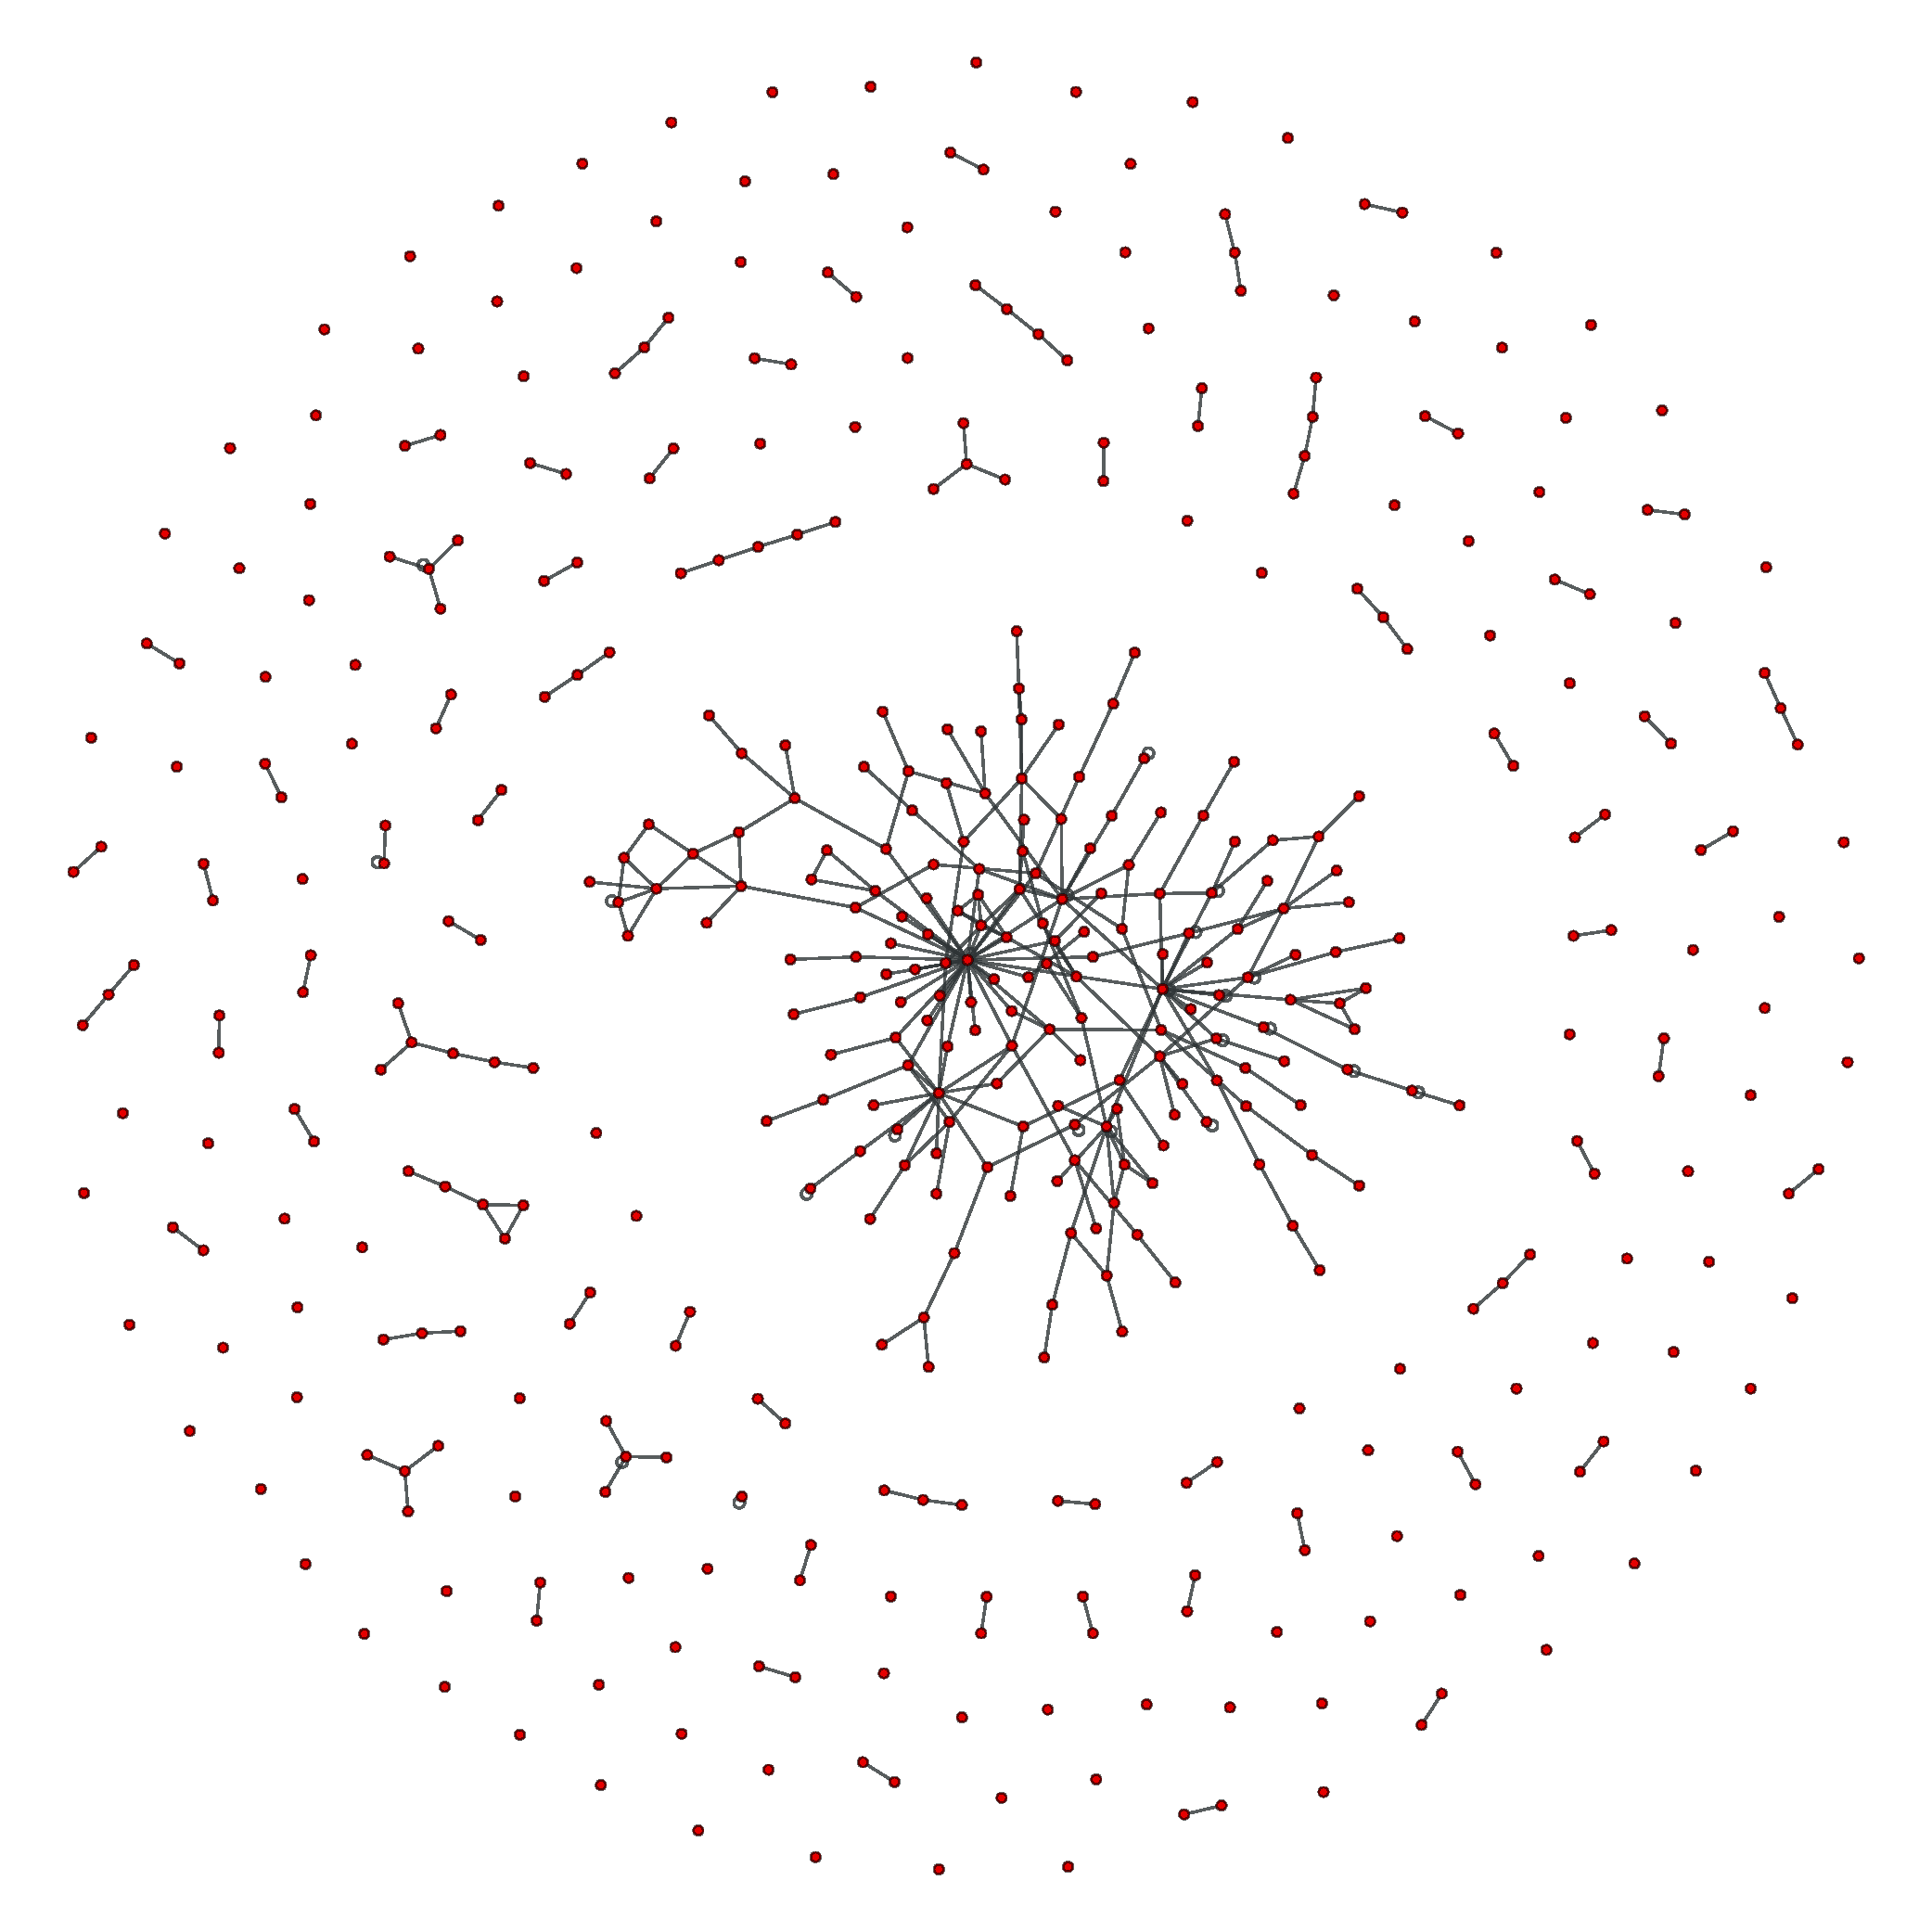
\includegraphics[width=.45\textwidth]{./schemes/subgrafo_Y2H_all-gml.pdf}\\
        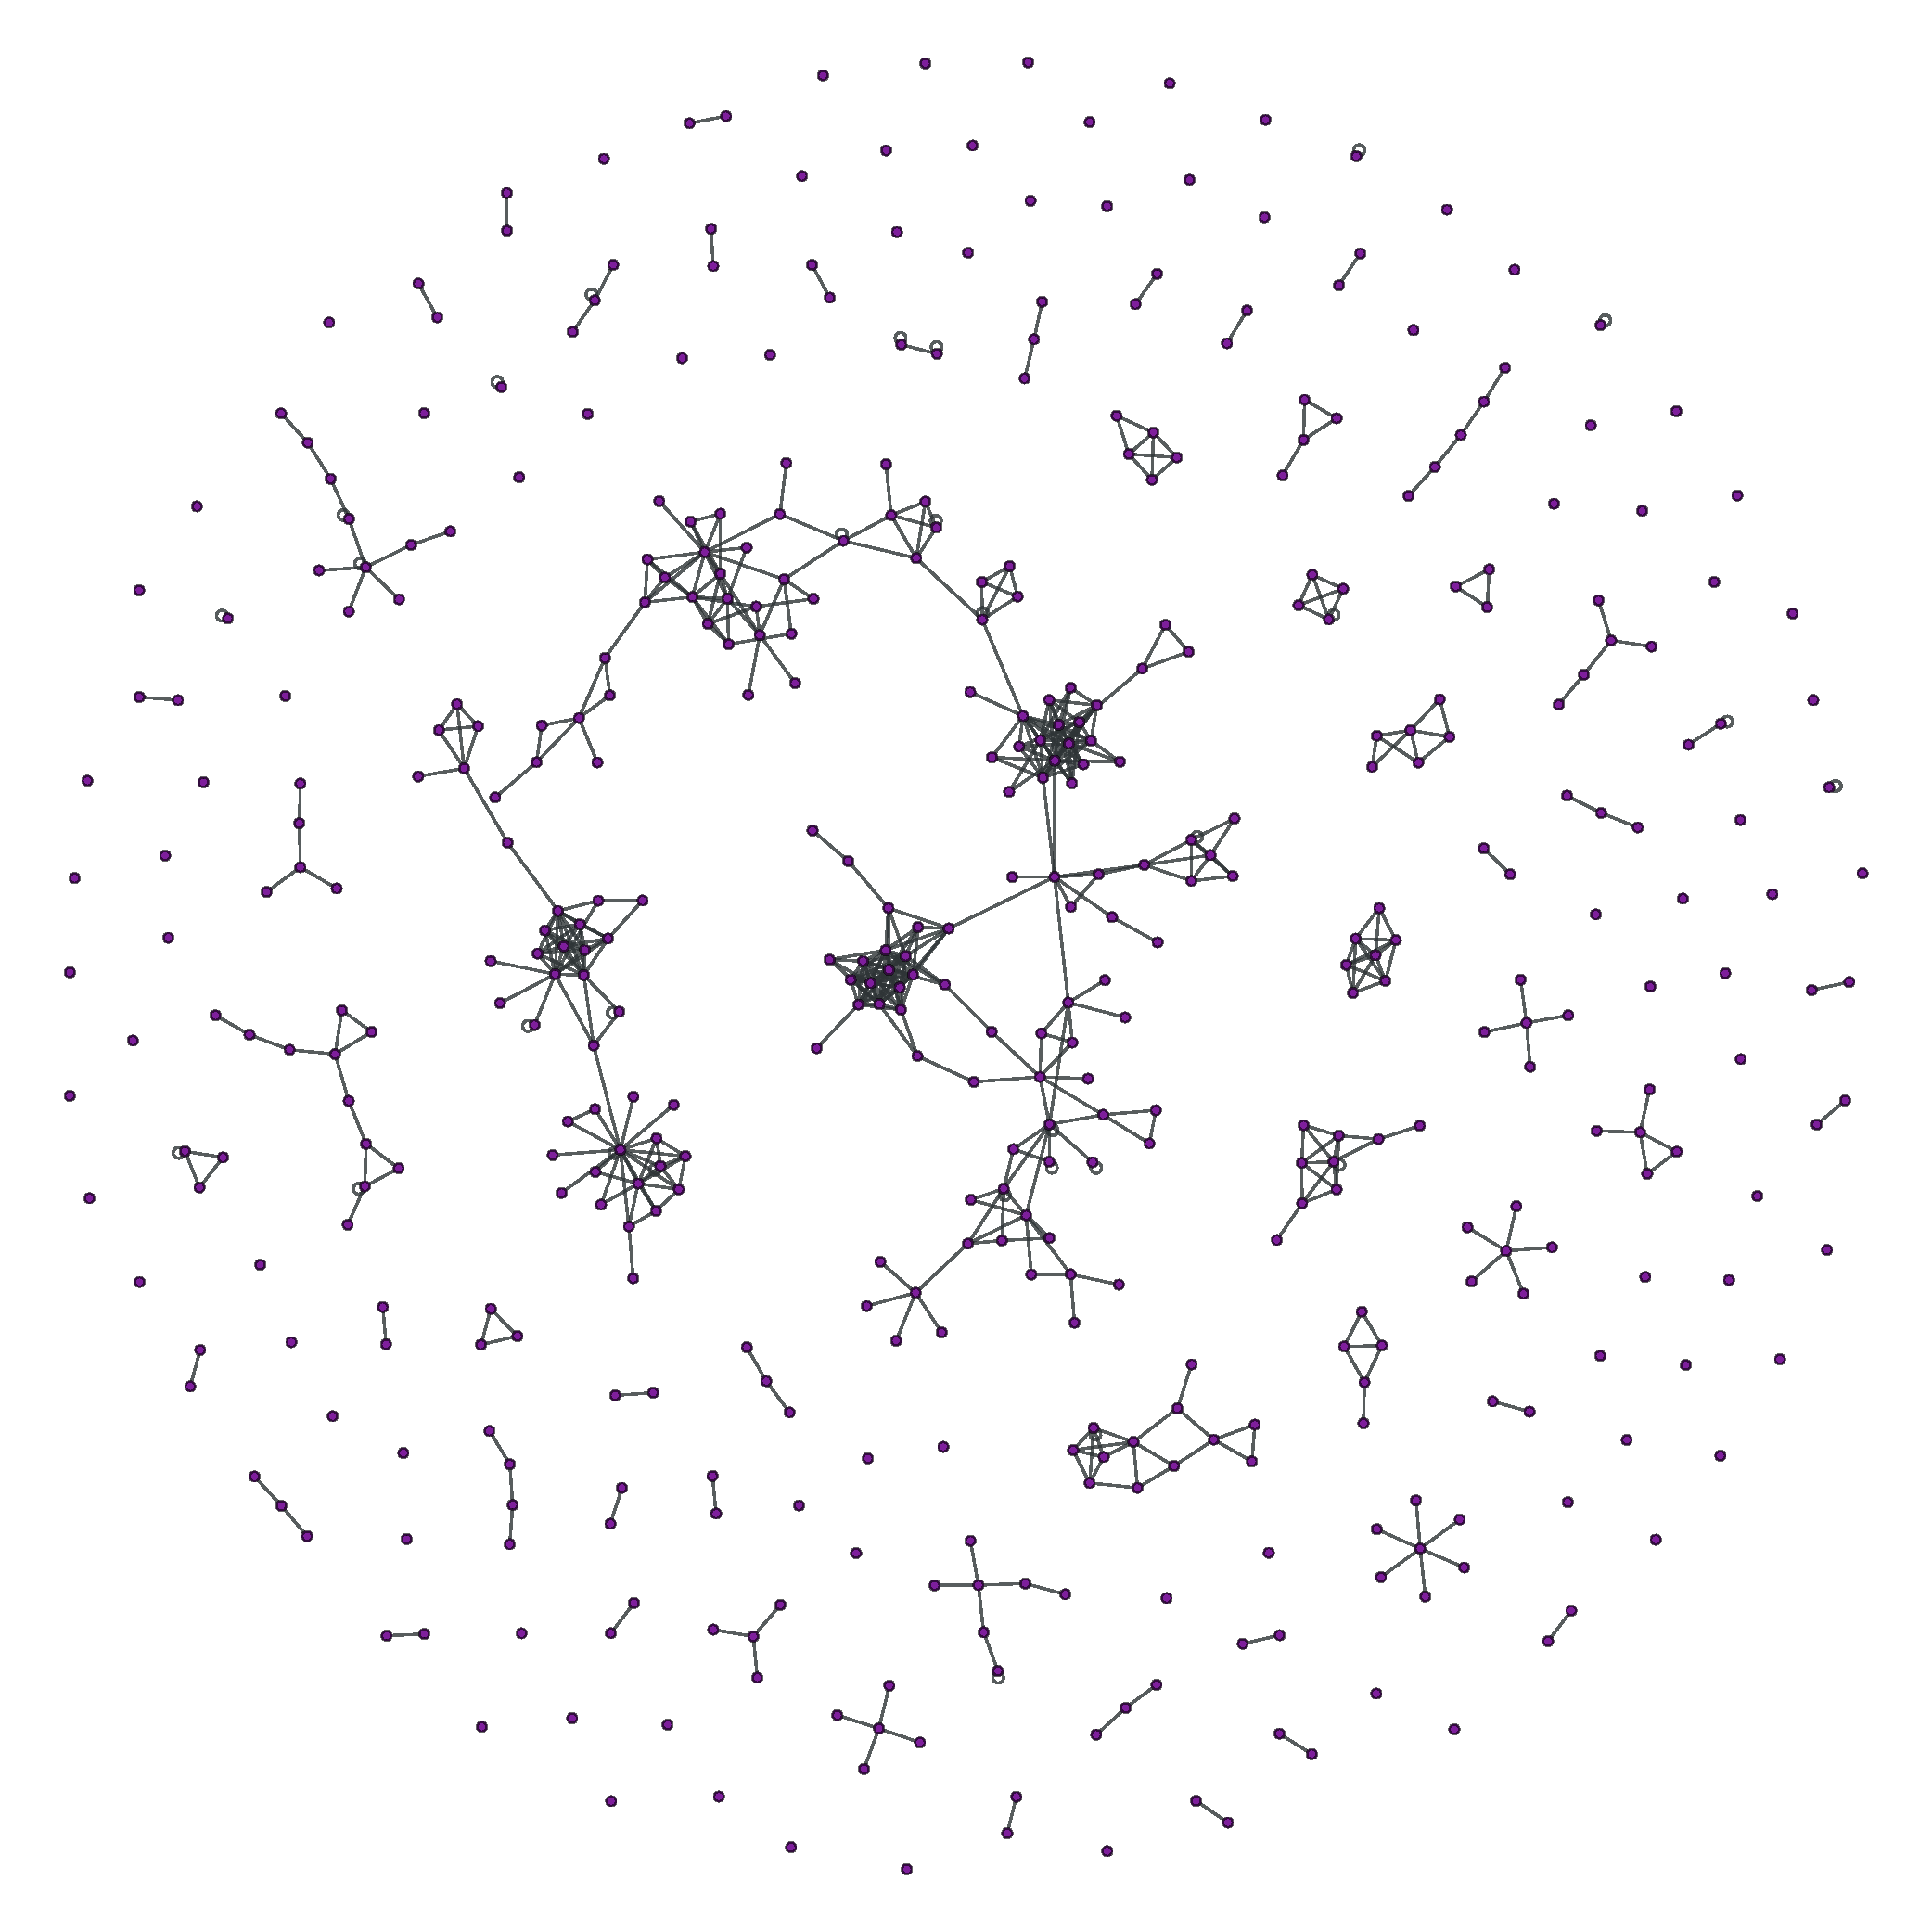
\includegraphics[width=.45\textwidth]{./schemes/subgrafo_LIT_all-gml.pdf}
        \caption{\label{fig:all} AP-MS/Y2H/LIT}
    \end{subfigure}
    \hfill
    \begin{subfigure}[b]{0.48\columnwidth}
        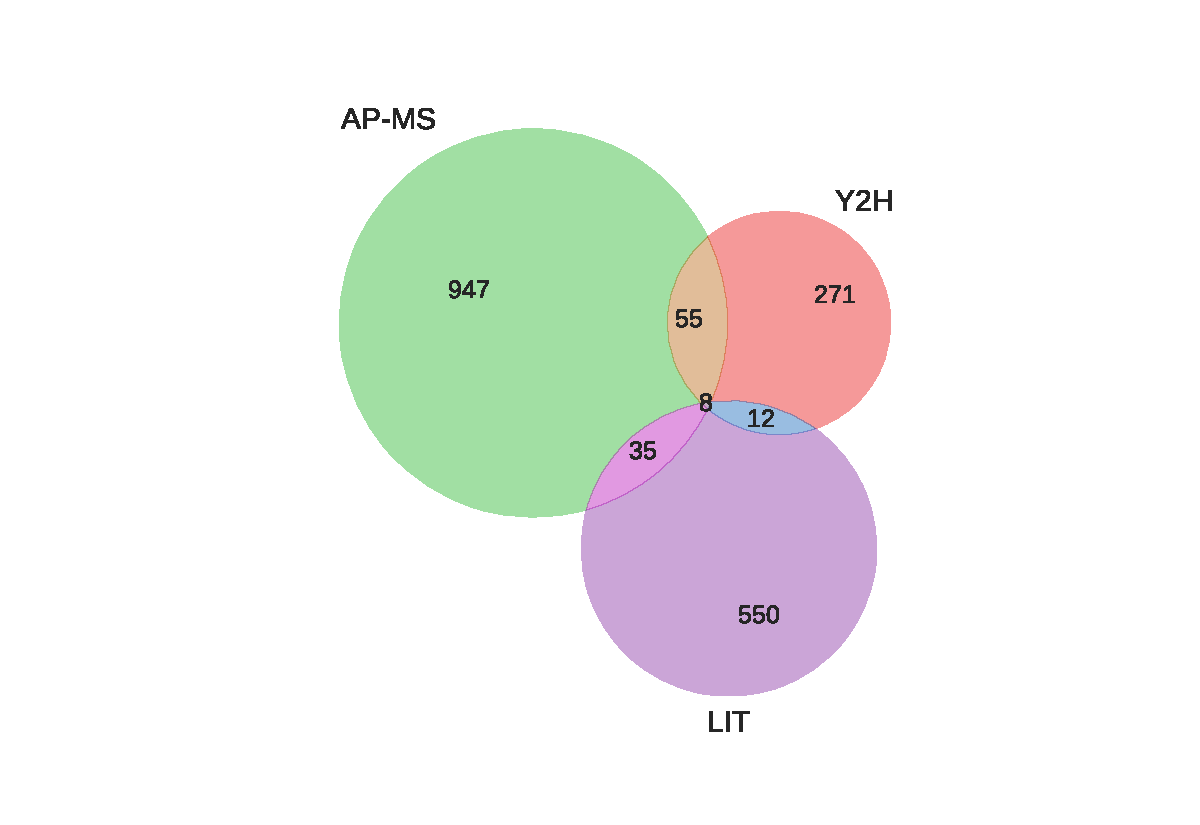
\includegraphics[width=\textwidth]{./schemes/venn_AP-MS-Y2H-LIT_links.pdf}
        \caption{\label{fig:cohe} Coherencia}
    \end{subfigure}
    \caption{\label{fig:venn} Subgrafos inducidos por cobertura de las 3 redes y coherencia de links entre ellas. }
\end{figure}

\vspace{1.5cm}
Por otra parte, a partir de la intersecci\'on de las prote\'inas reportadas de las tres redes, se analiza la coherencia
de los enlaces entre las prote\'inas comunes. De la figura \ref{fig:cohe} se puede observar al alta especificidad
de cada red respecto al resto (solo 8 links son compartidos por las tres redes). 


\begin{figure}[!ht]
    \centering
    \begin{subfigure}[b]{0.3\columnwidth}
        \centering
        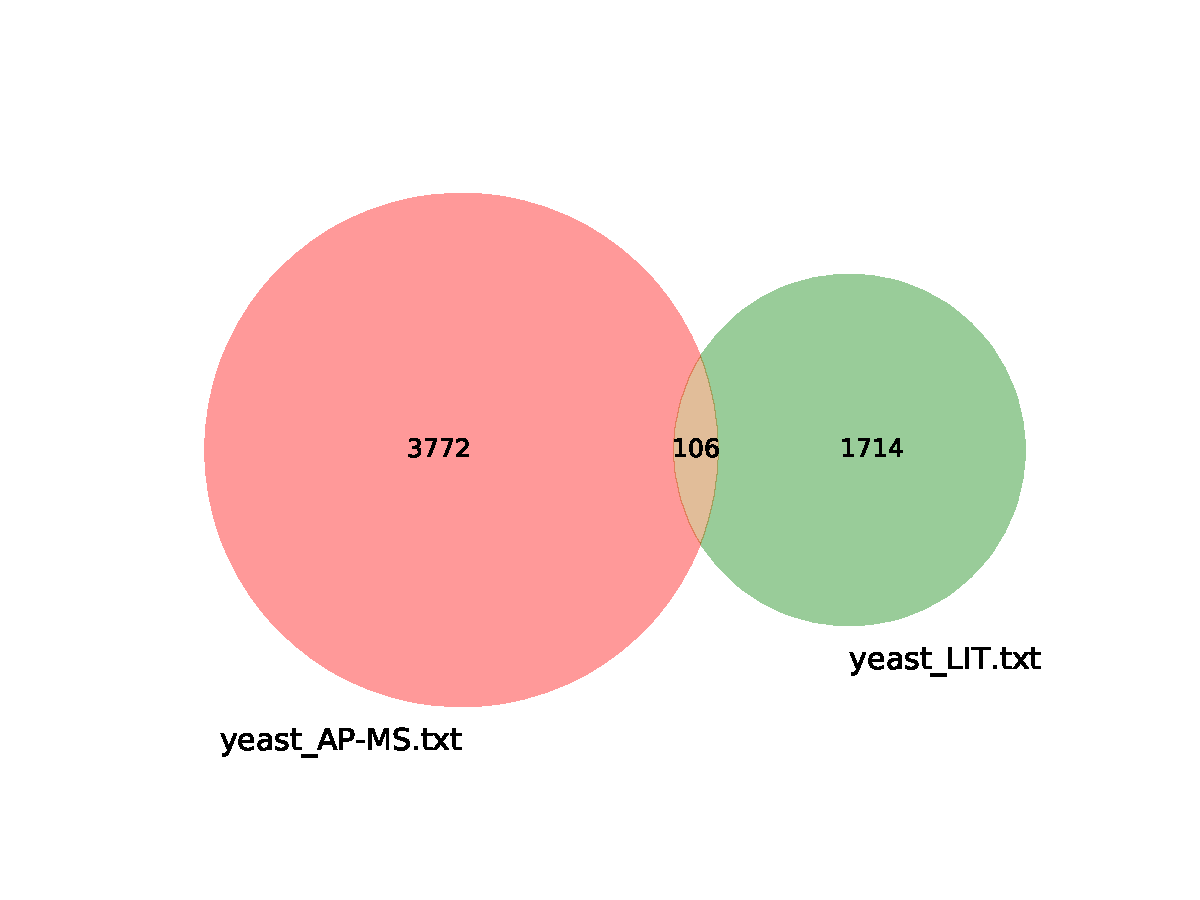
\includegraphics[width=.7\textwidth]{./schemes/venn2_coherence_yeast_AP-MS-yeast_LIT.pdf}\\
        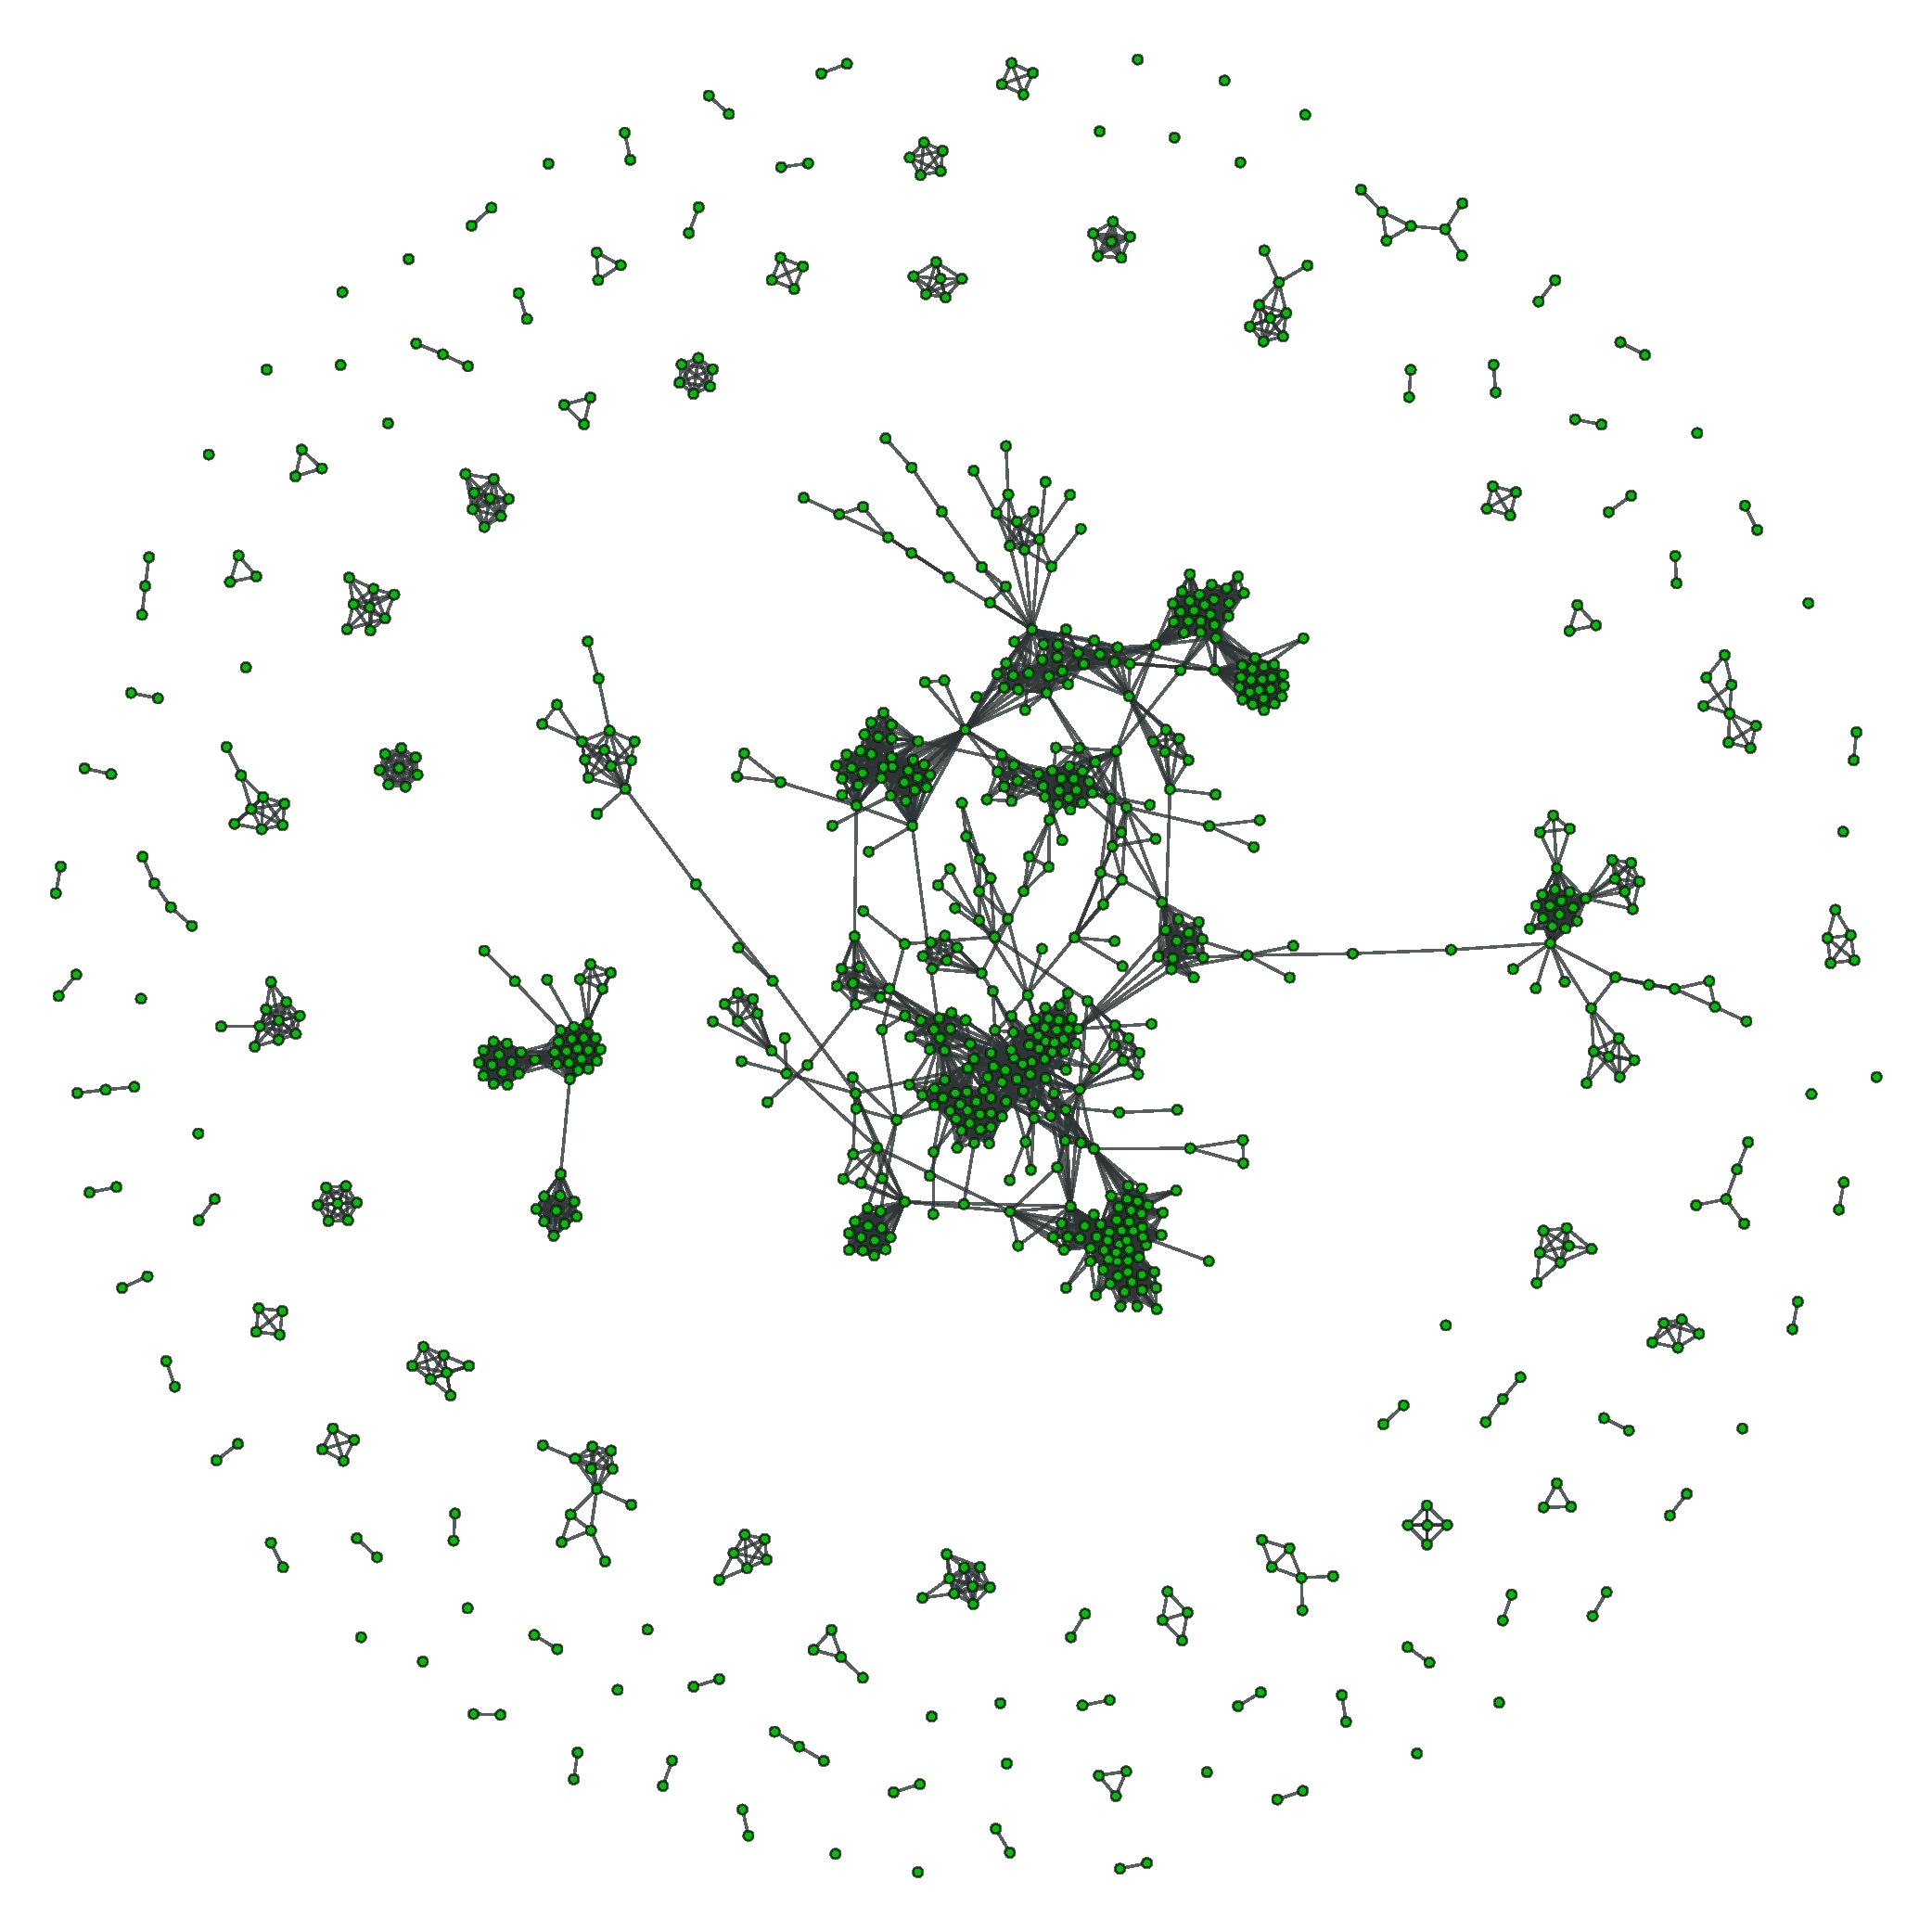
\includegraphics[width=.45\textwidth]{./schemes/subgrafo_APMS_ap_ms_lit-gml.pdf}
        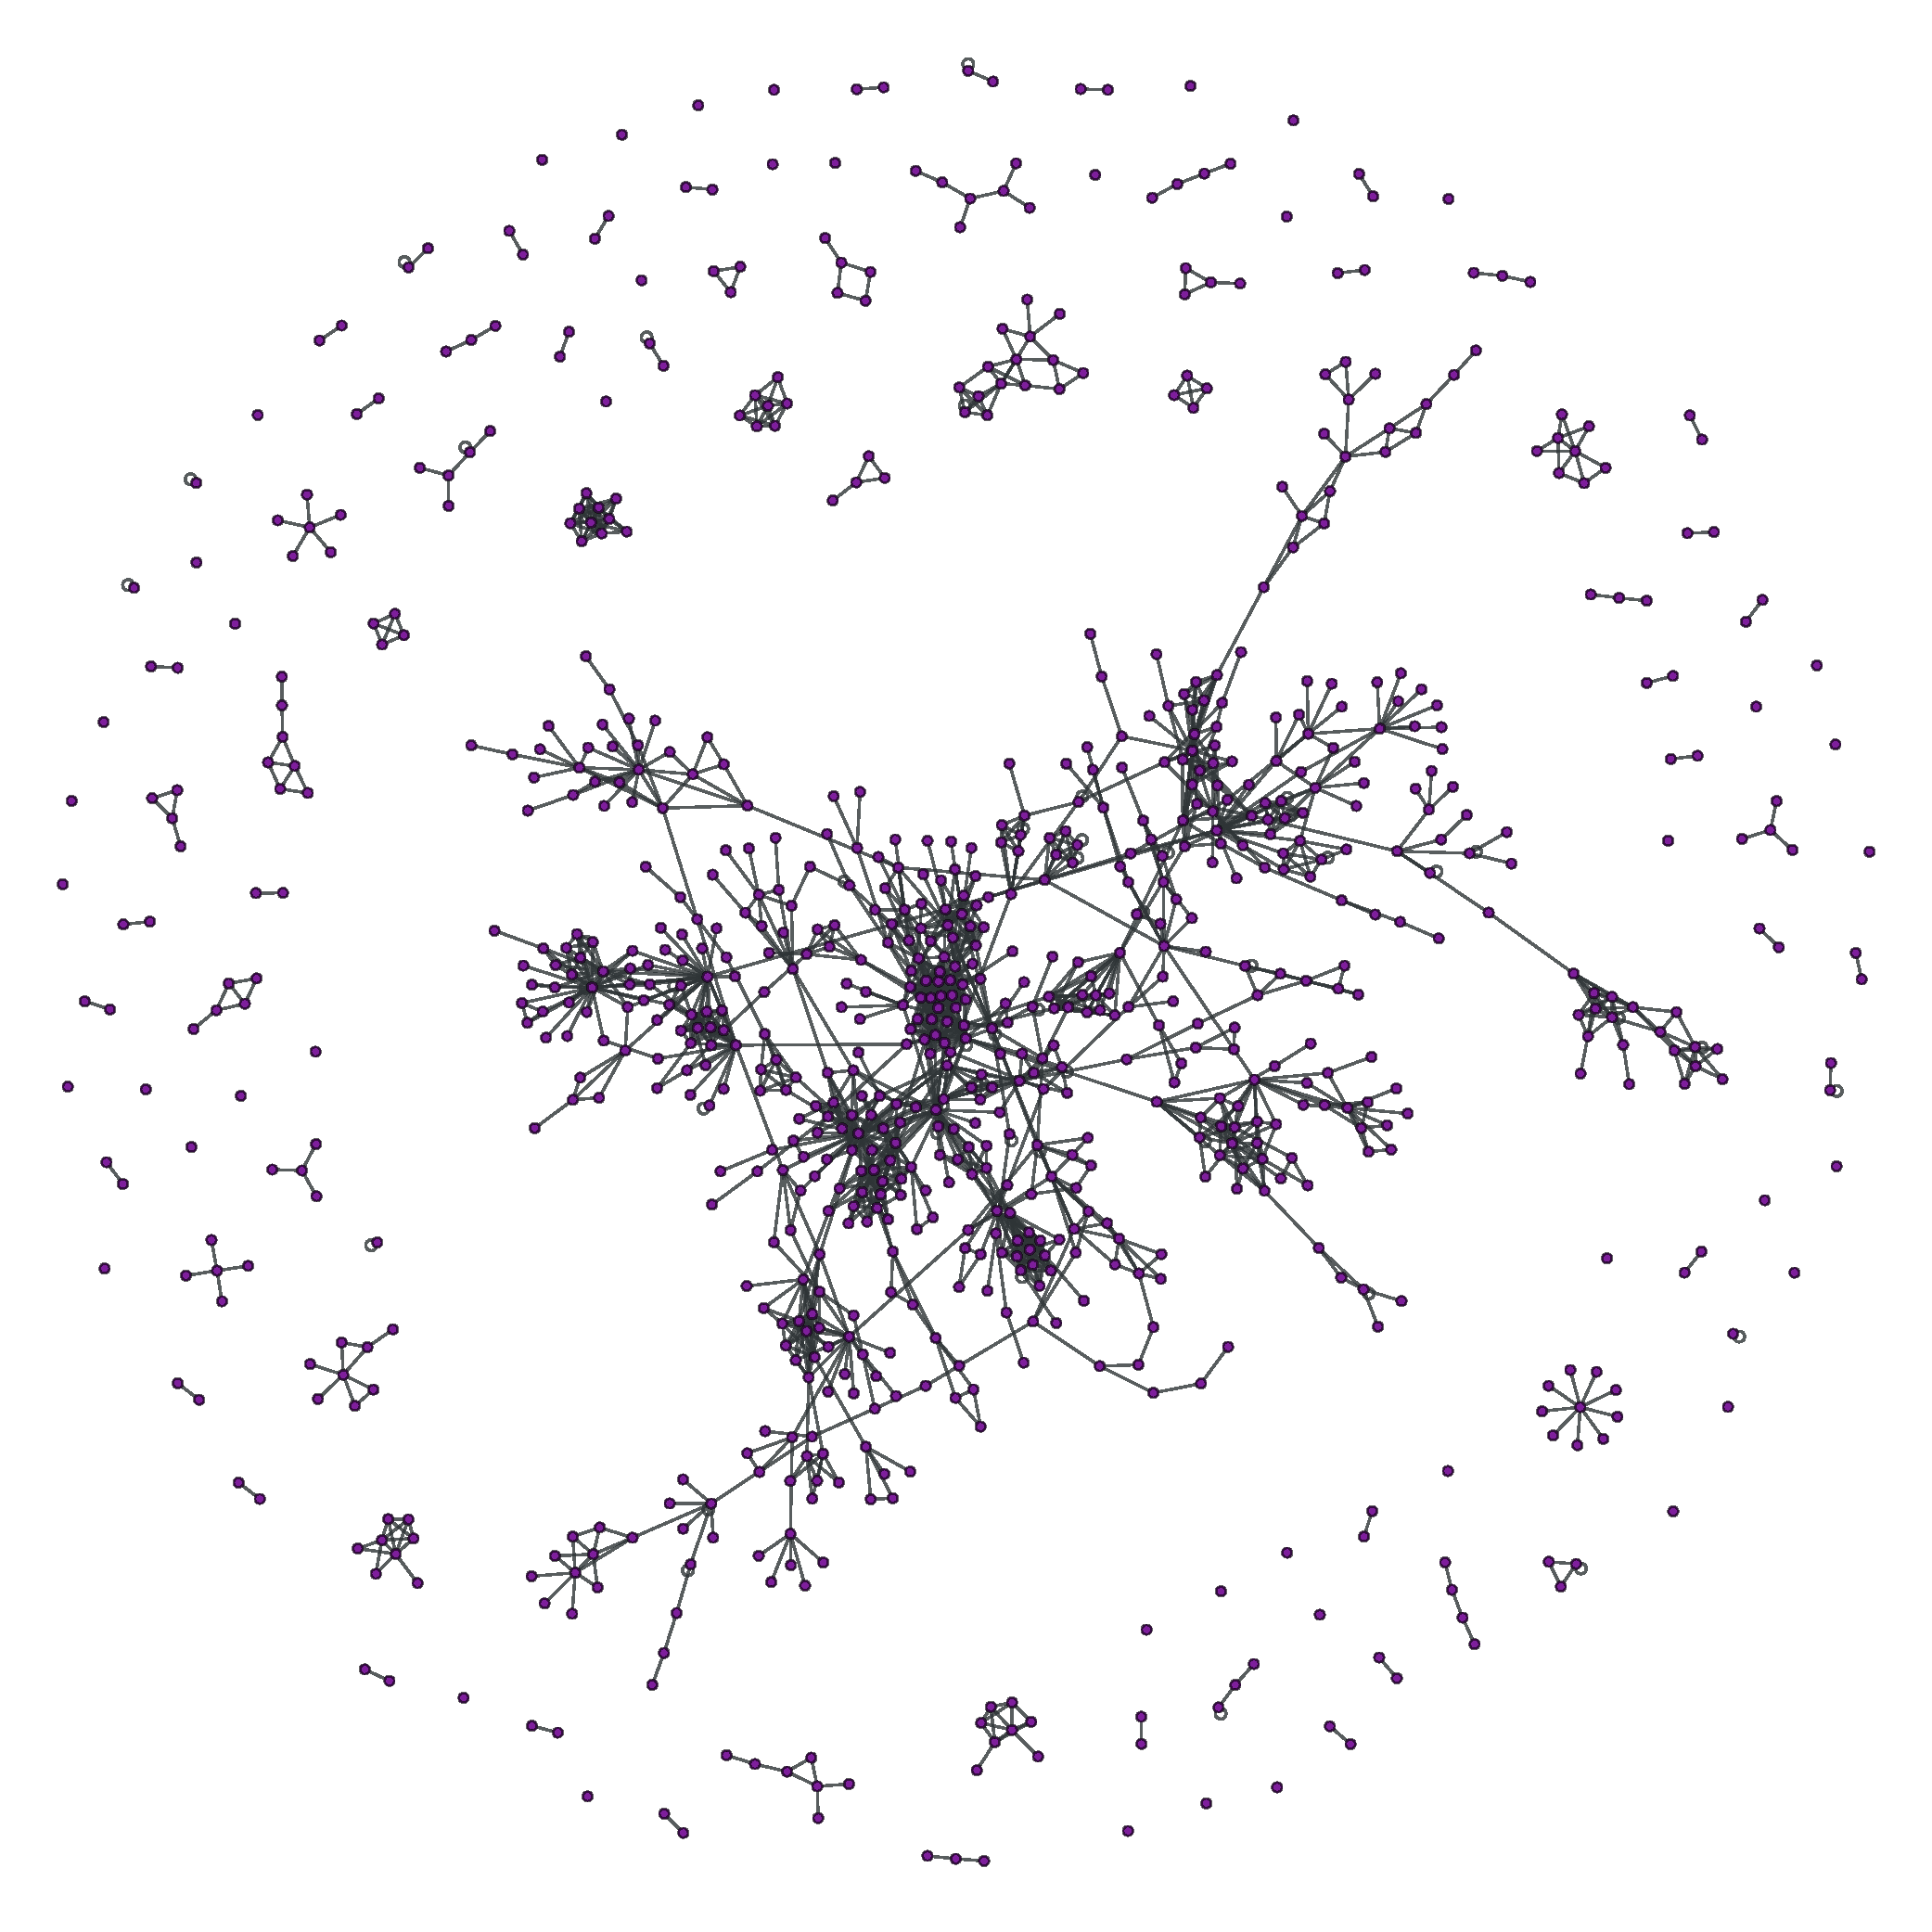
\includegraphics[width=.45\textwidth]{./schemes/subgrafo_LIT_ap_ms_lit-gml.pdf}
        \caption{\label{fig:apms-lit} AP-MS/LIT}
    \end{subfigure}
    \begin{subfigure}[b]{0.3\columnwidth}
        \centering
        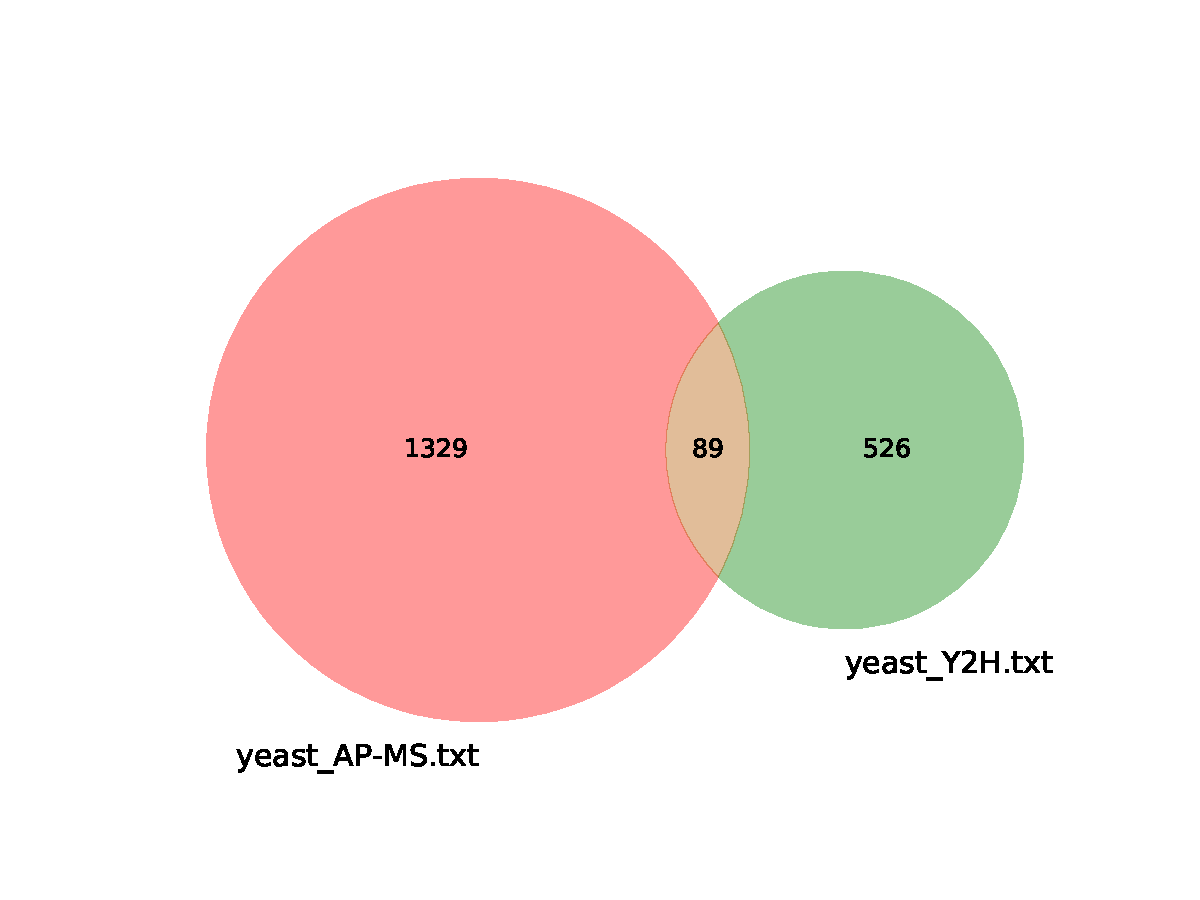
\includegraphics[width=.7\textwidth]{./schemes/venn2_coherence_yeast_AP-MS-yeast_Y2H.pdf}\\
        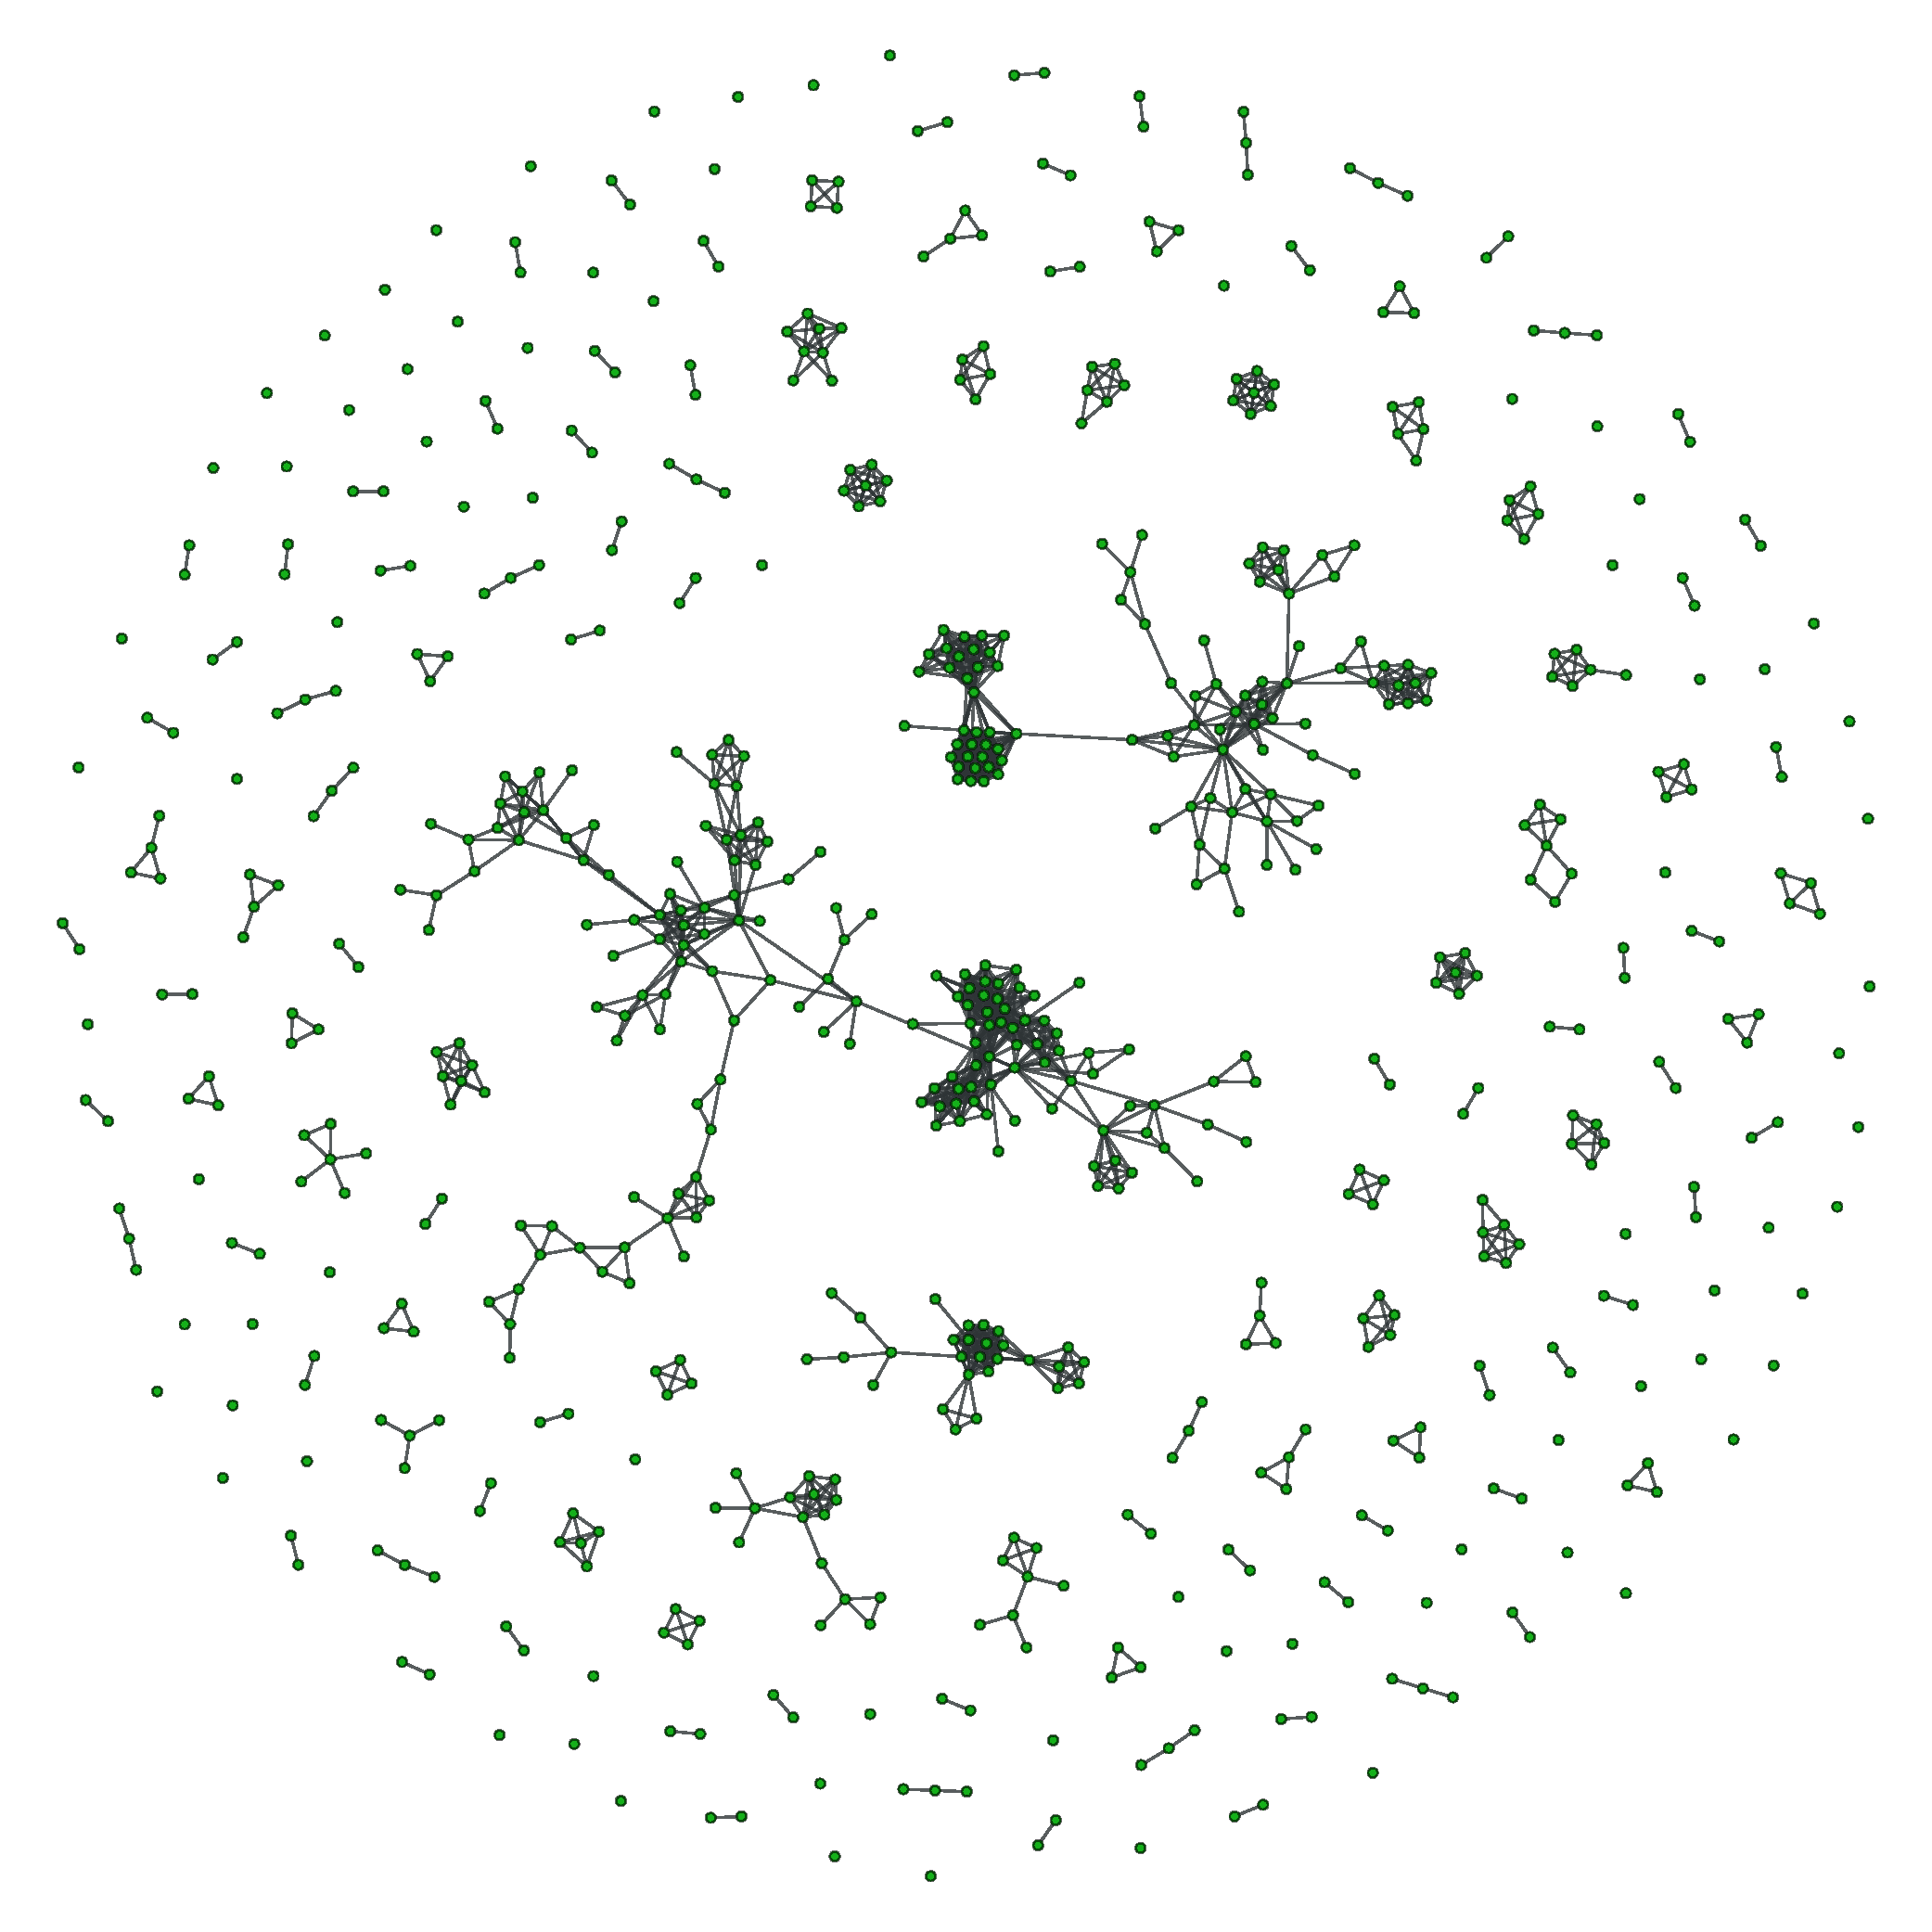
\includegraphics[width=.45\textwidth]{./schemes/subgrafo_APMS_ap_ms_y2h-gml.pdf}
        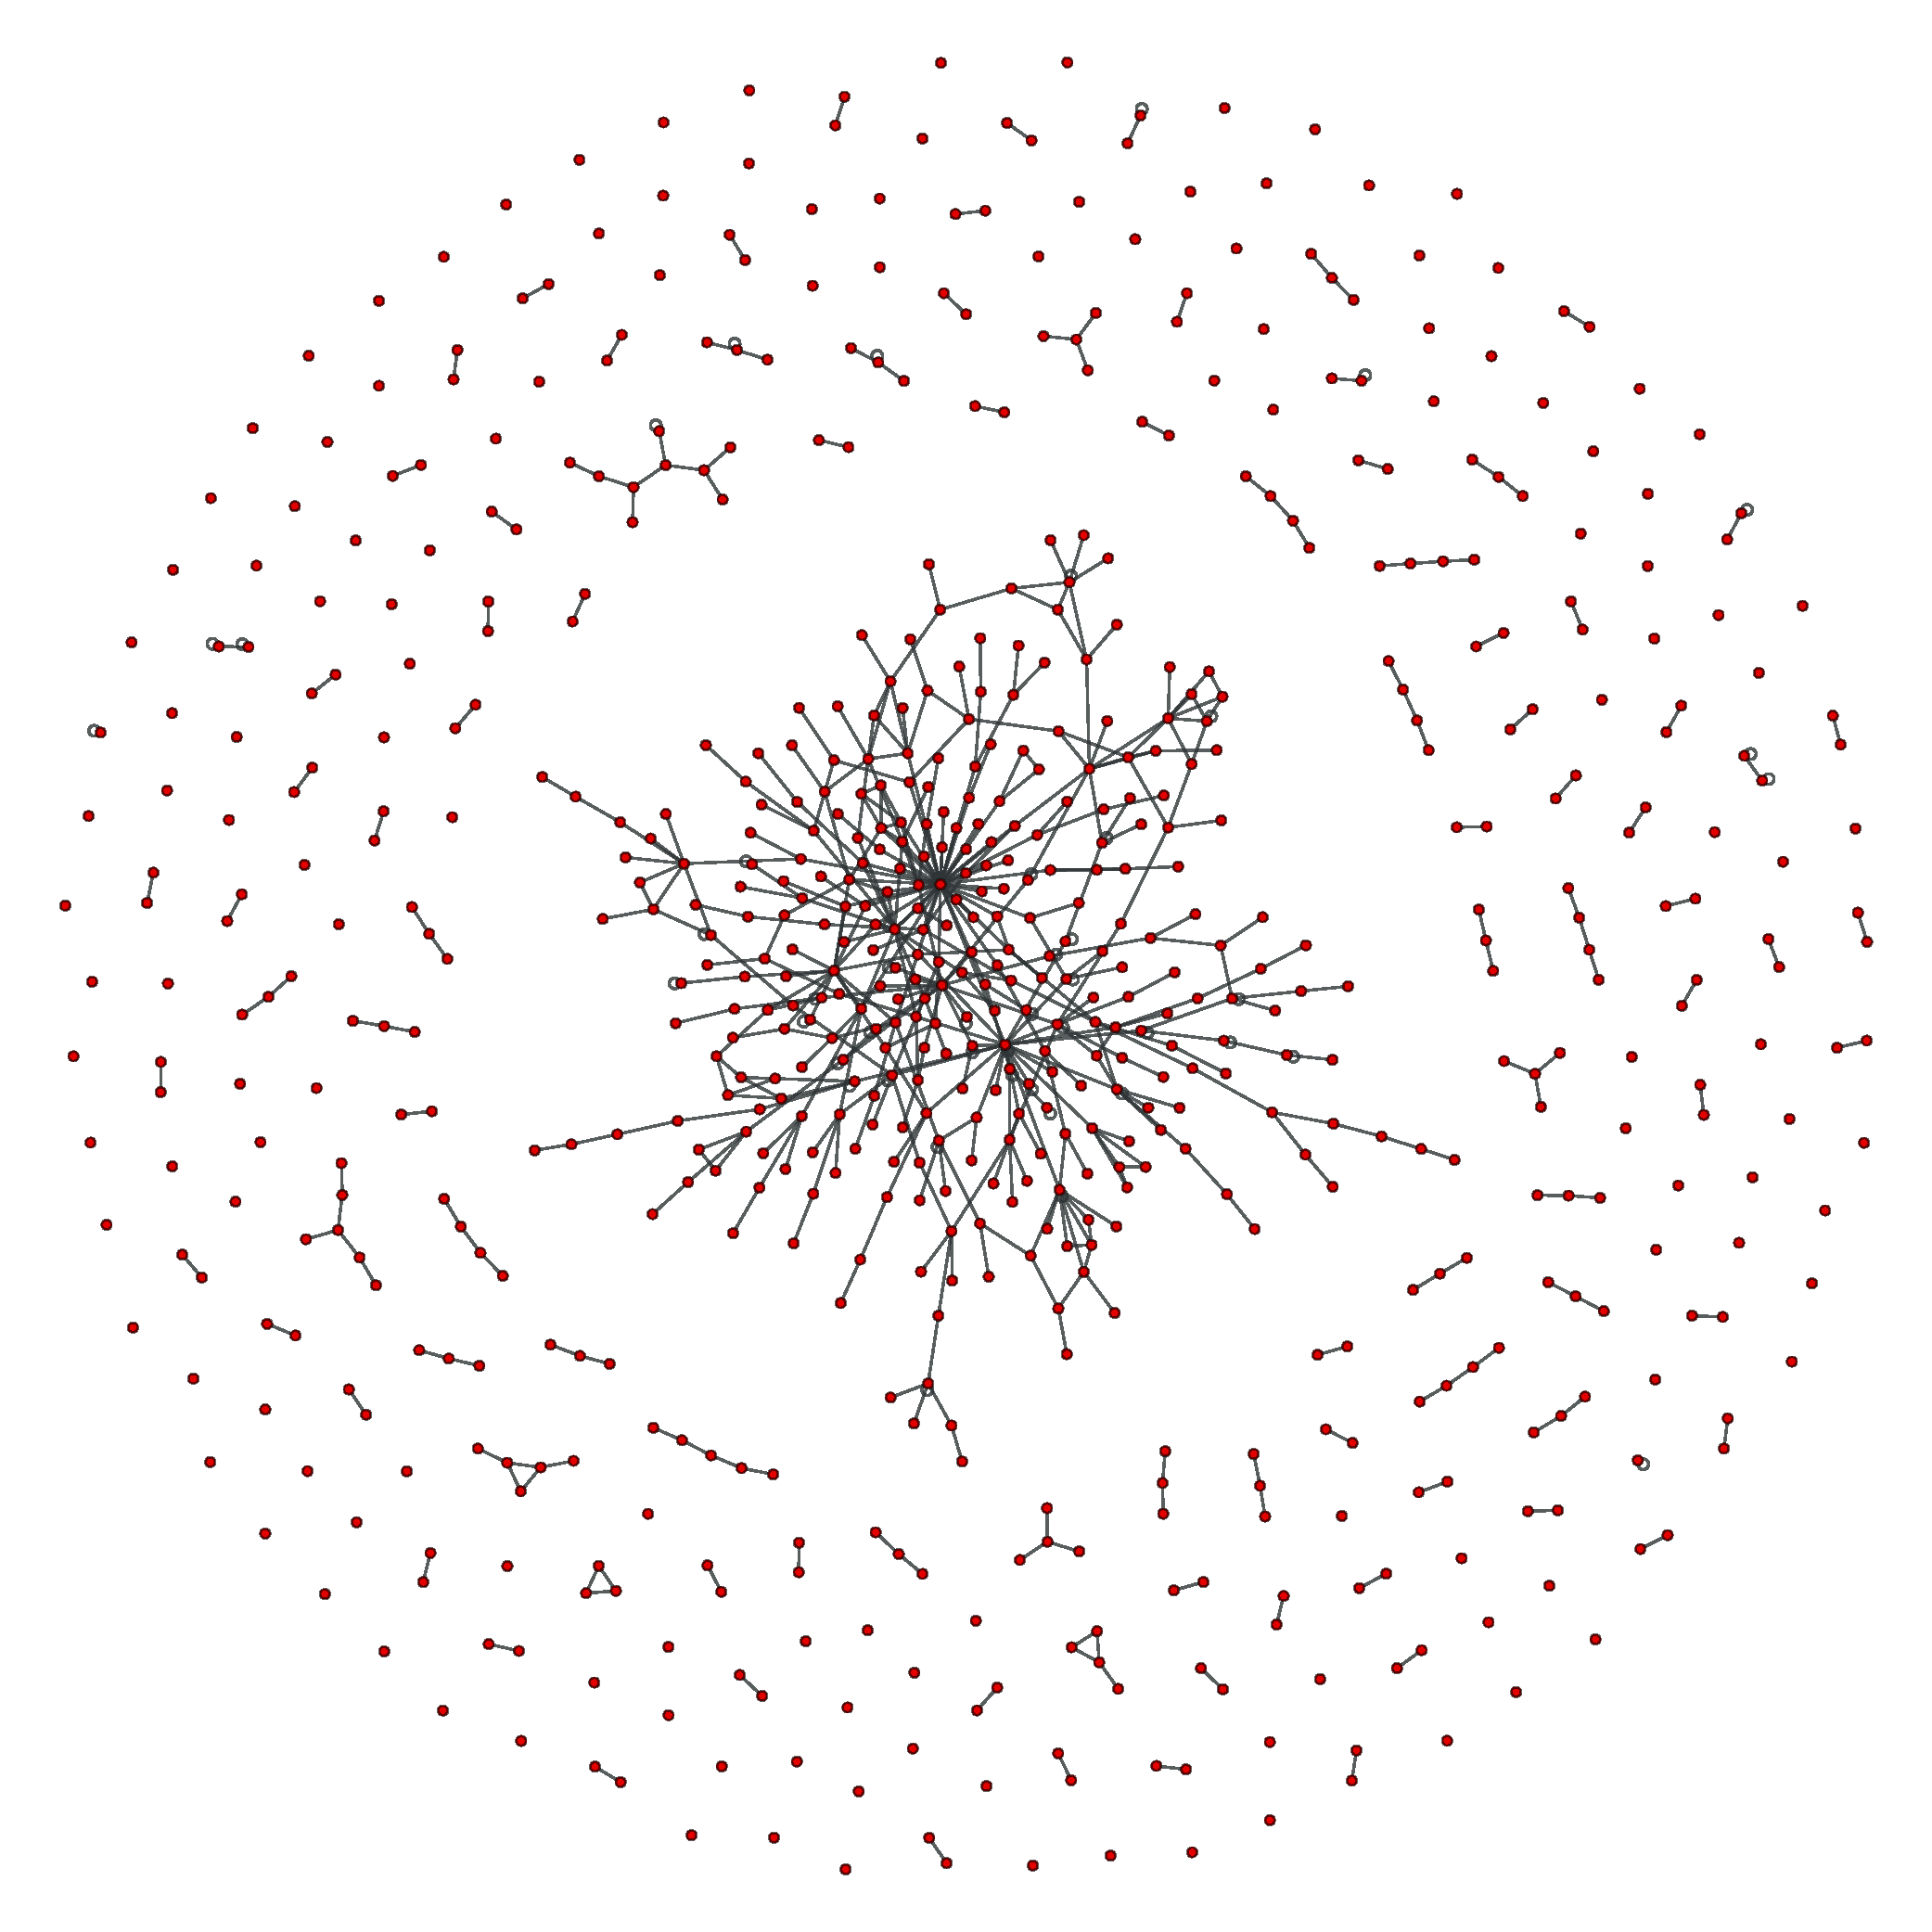
\includegraphics[width=.45\textwidth]{./schemes/subgrafo_Y2H_ap_ms_y2h-gml.pdf}
        \caption{\label{fig:apms-y2h} AP-MS/Y2H}
    \end{subfigure}
    \begin{subfigure}[b]{0.3\columnwidth}
        \centering
        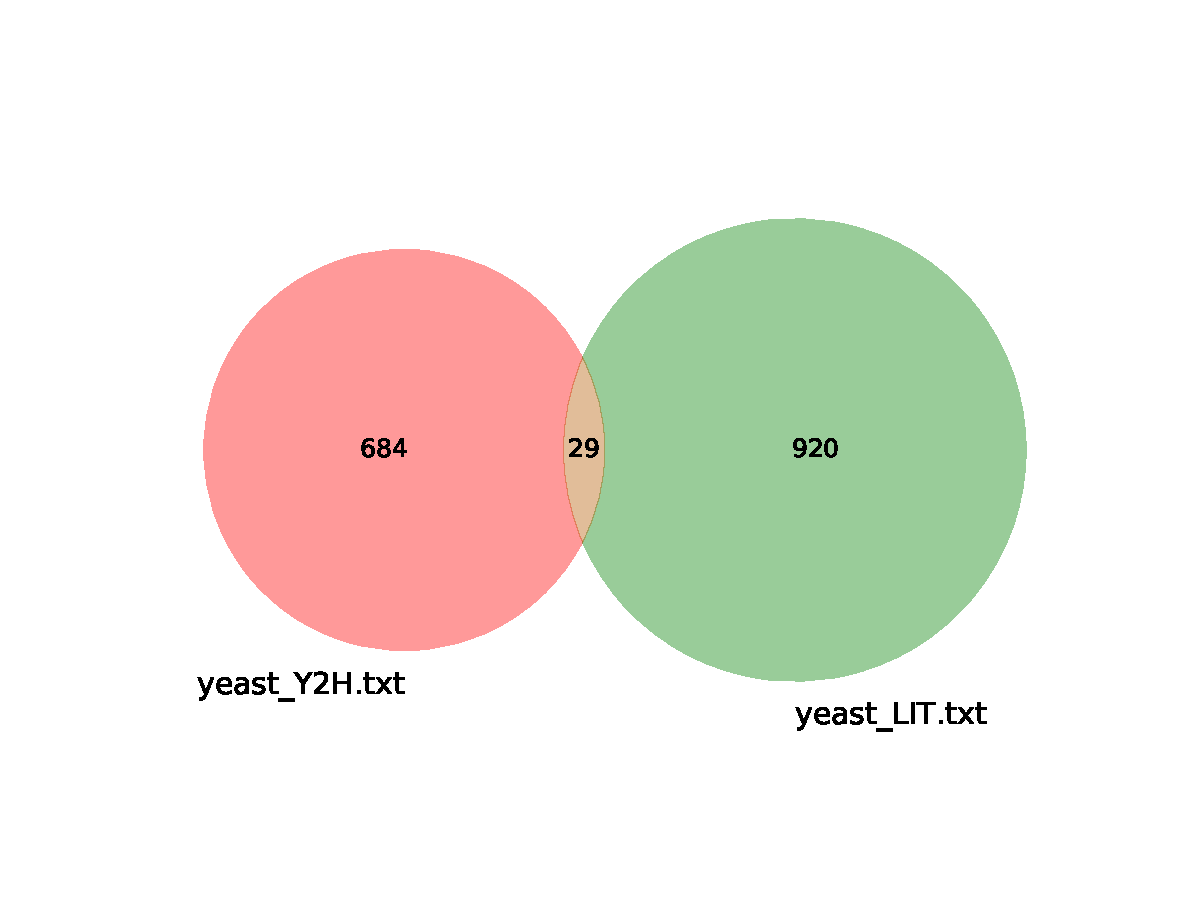
\includegraphics[width=.7\textwidth]{./schemes/venn2_coherence_yeast_Y2H-yeast_LIT.pdf}\\
        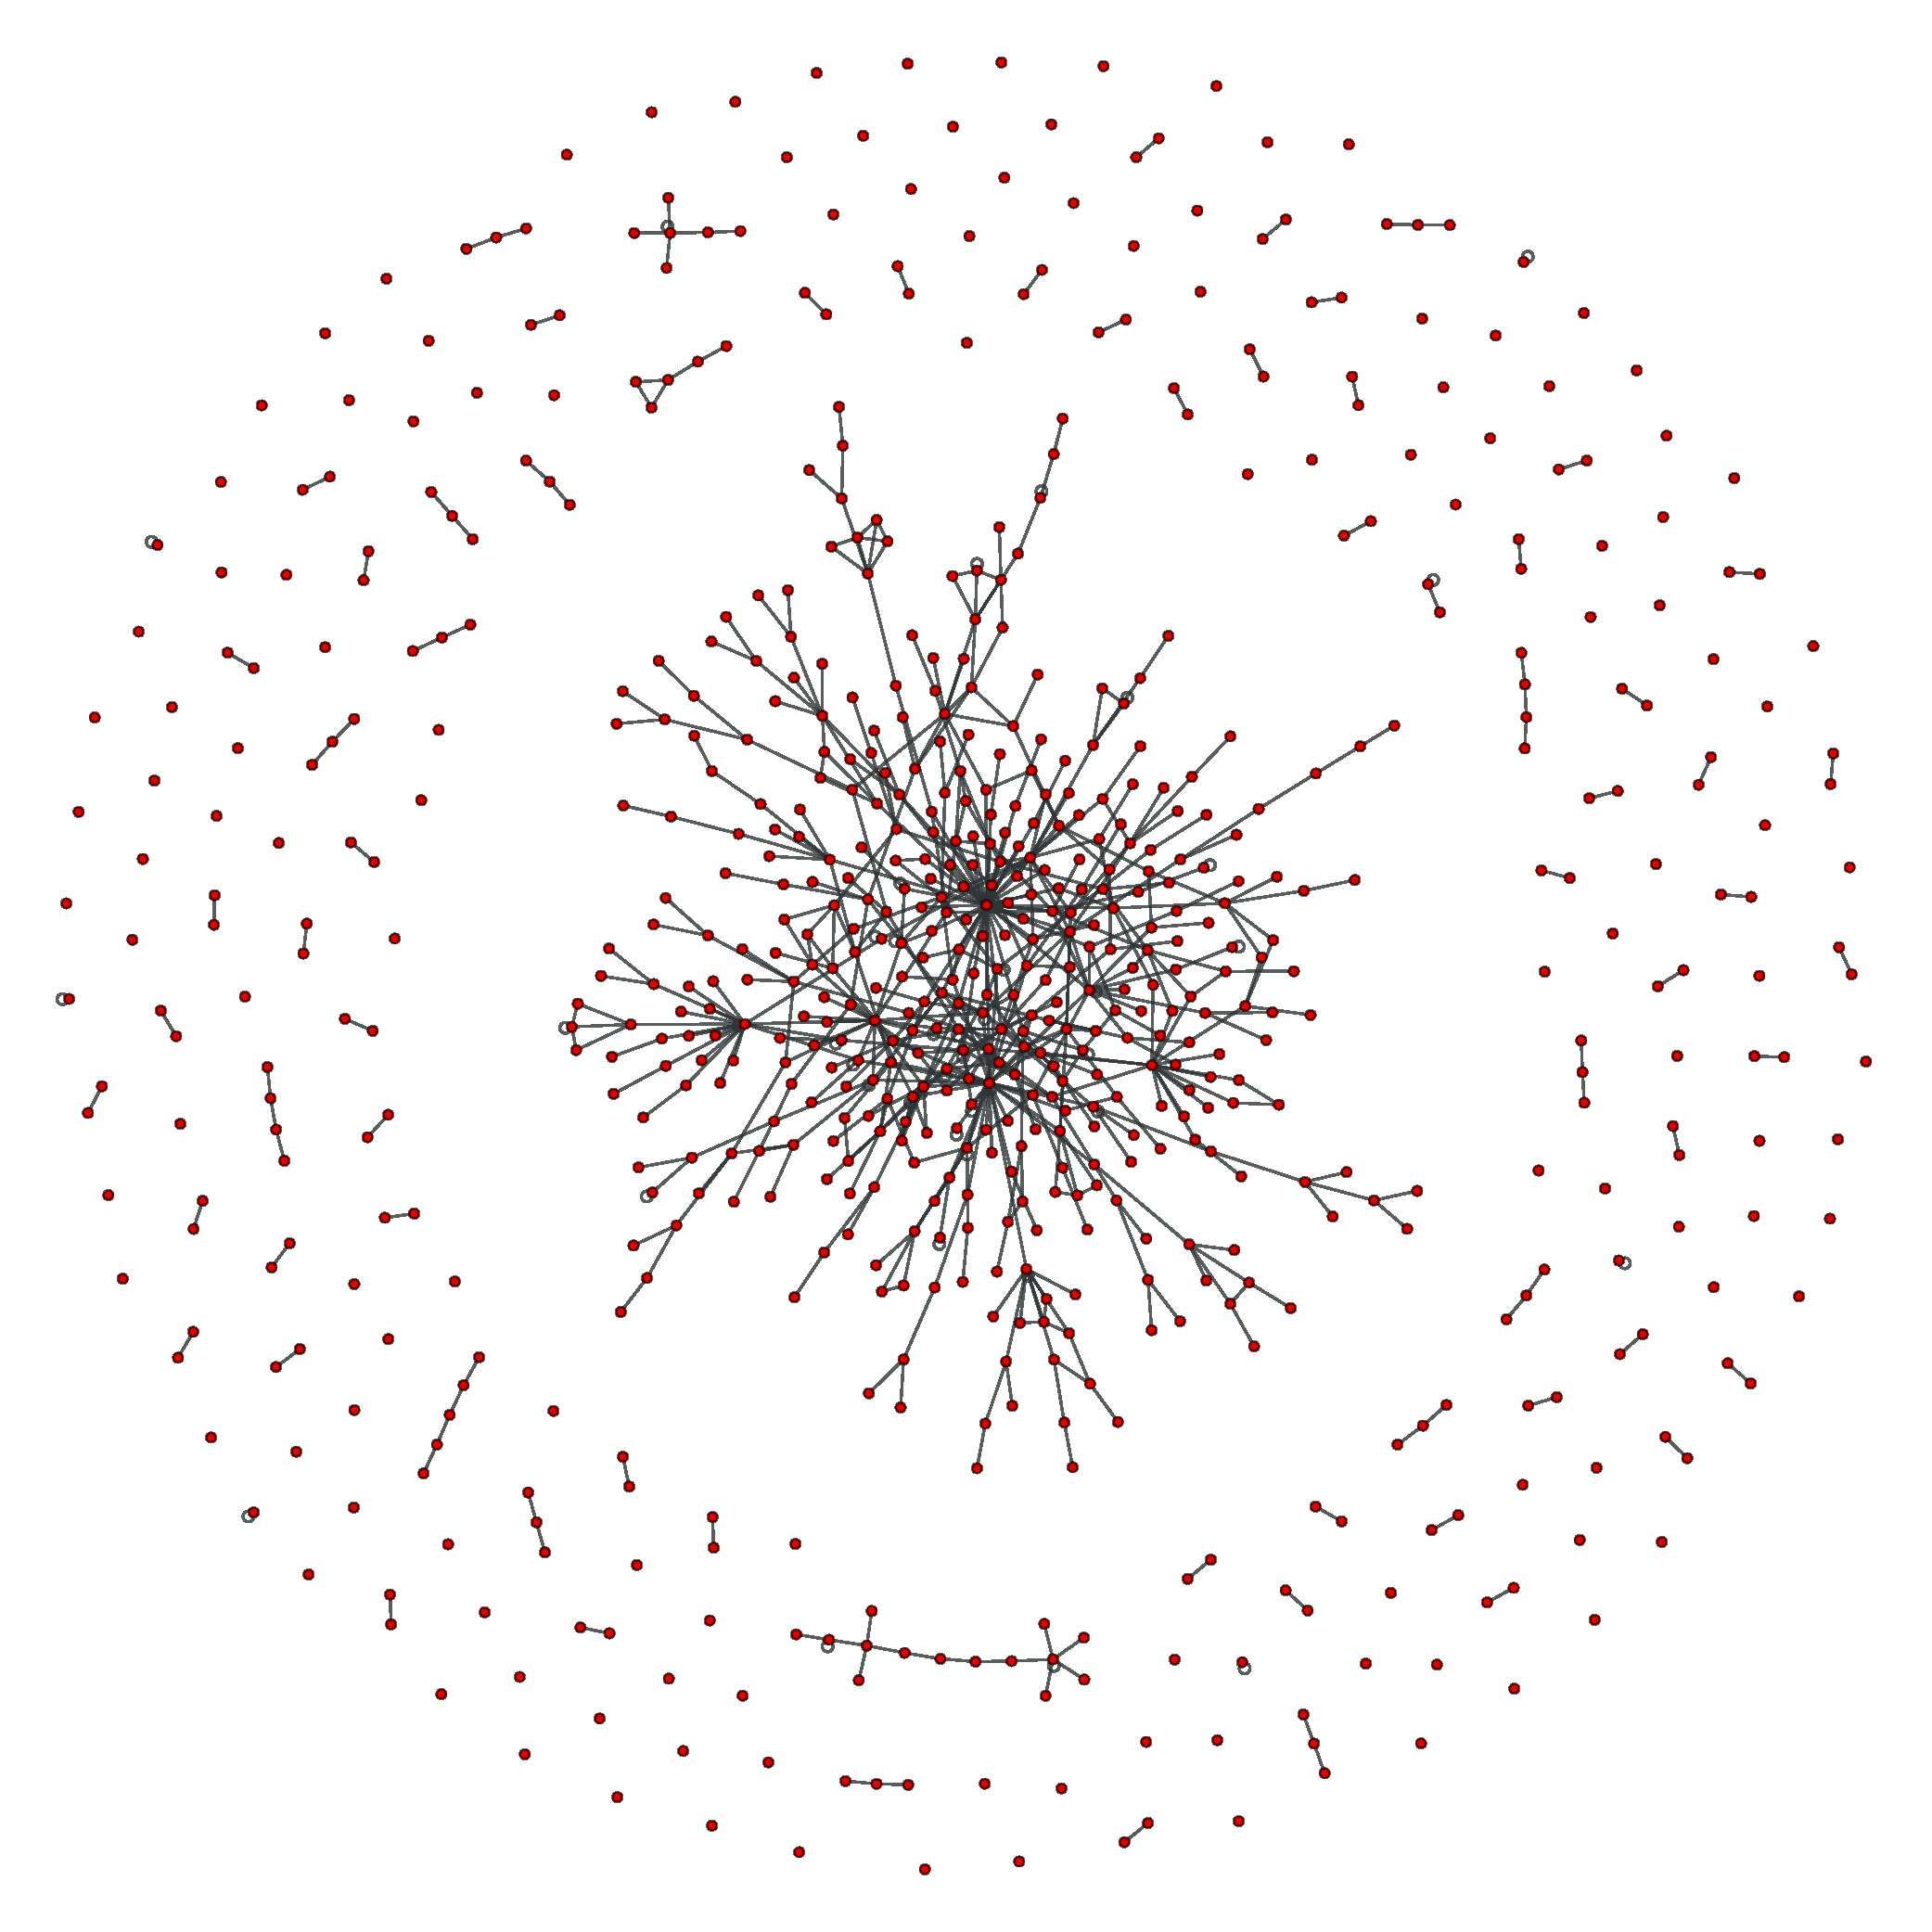
\includegraphics[width=.45\textwidth]{./schemes/subgrafo_Y2H_y2h_lit-gml.pdf}
        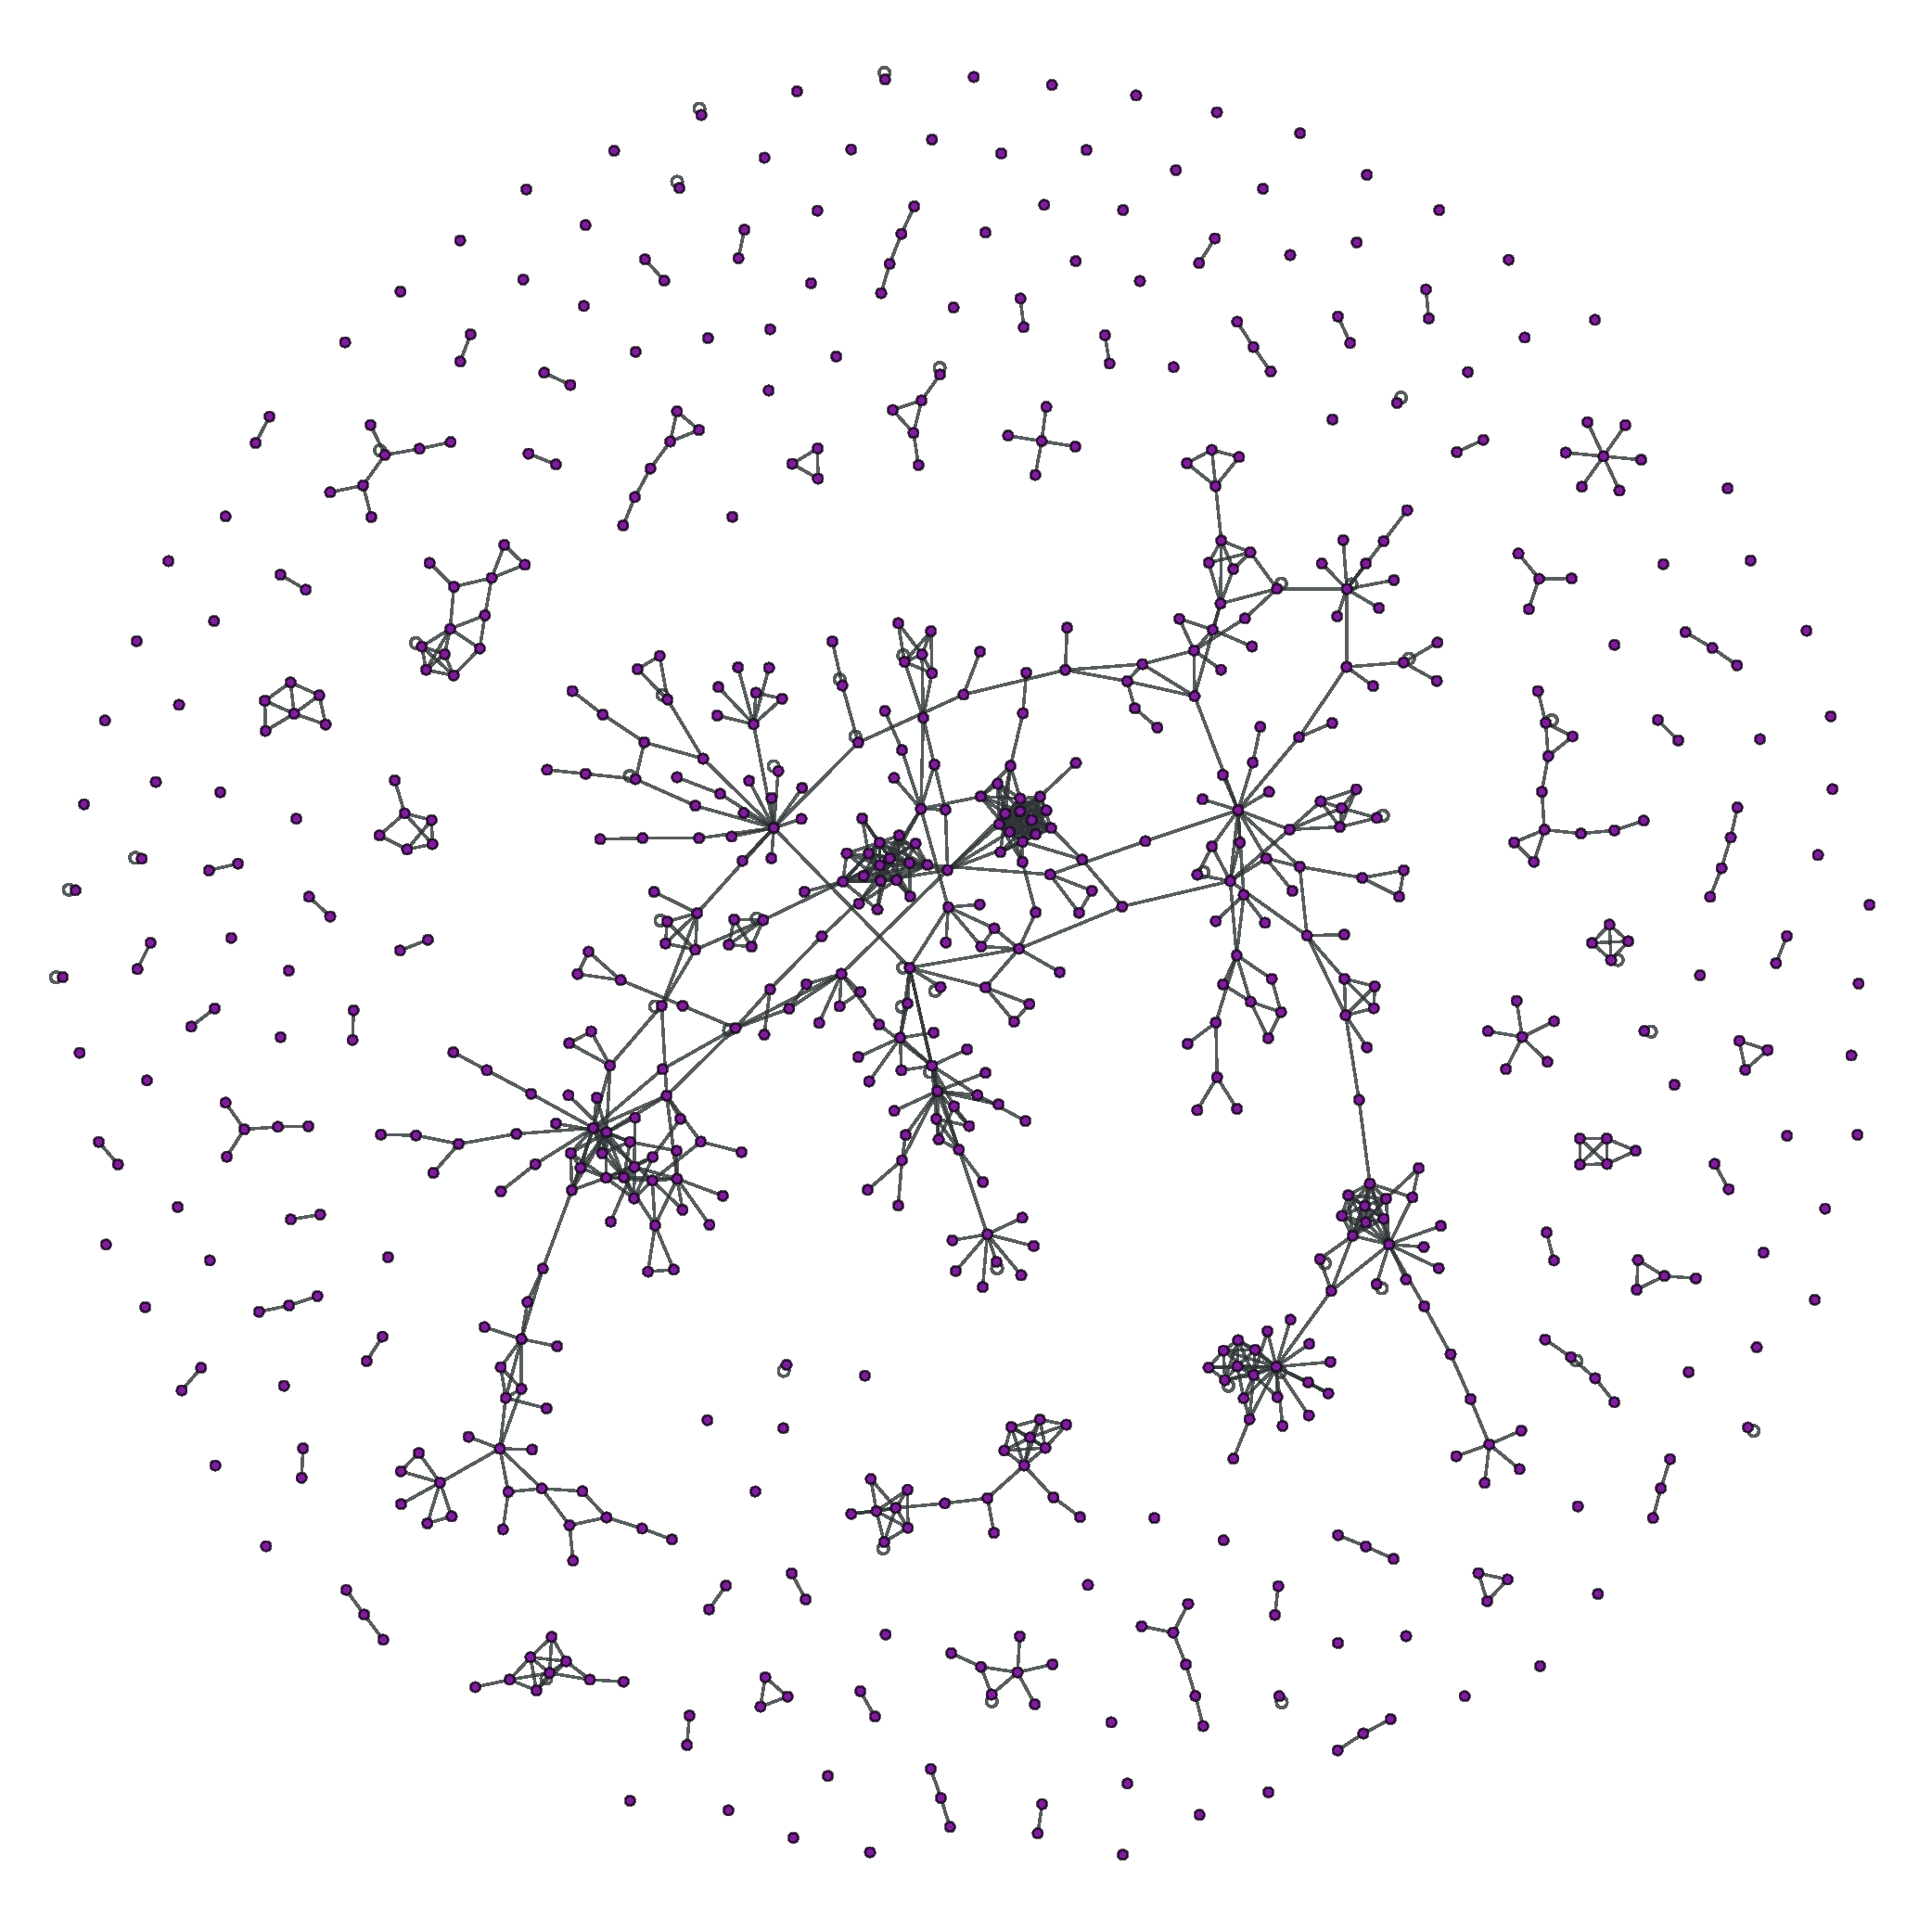
\includegraphics[width=.45\textwidth]{./schemes/subgrafo_LIT_y2h_lit-gml.pdf}
        \caption{\label{fig:y2h-lit} Y2H/LIT}
    \end{subfigure}
    \caption{\label{fig:subgrafos} Coherencia entre links para cada par de redes y los respectivos subgrafos de cada red }
\end{figure}

Adicionalmente se muestran las coherencias
a pares y los subgrafos inducidos en la figura~\ref{fig:subgrafos}. Cabe notar que, a pesar que en los subgrafos
de la cobertura entre AP-MS y LIT podr\'ian parecer \textit{similares}, las coherencias entre links en todos los casos son
escasas respecto a la cantidad total de links en cada subgrafo.



\section{Ejercicio 2.}

La red de este ejercicio trata de una comunidad de delfines de Doubtful Sound, Nueva Zelanda. La comunidad, que se constituye de 62 ejemplares identificados por una marca en la aleta dorsal, fue fotografiada entre 1995 y 2001. A partir de esos datos se construyó la red que contiene 159 links, donde se establece que existe un link entre aquellos individuos que fueron vistos juntos de forma más frecuente que la esperada aleatoriamente, es decir, por un criterio de ``compañía preferida". [D. Lusseau, The emergent properties of a dolphin social network, Proc. R. Soc. London B (suppl.) 270, S186-S188 (2003).]

\subsection{Parte a.}

\begin{figure}
\centering
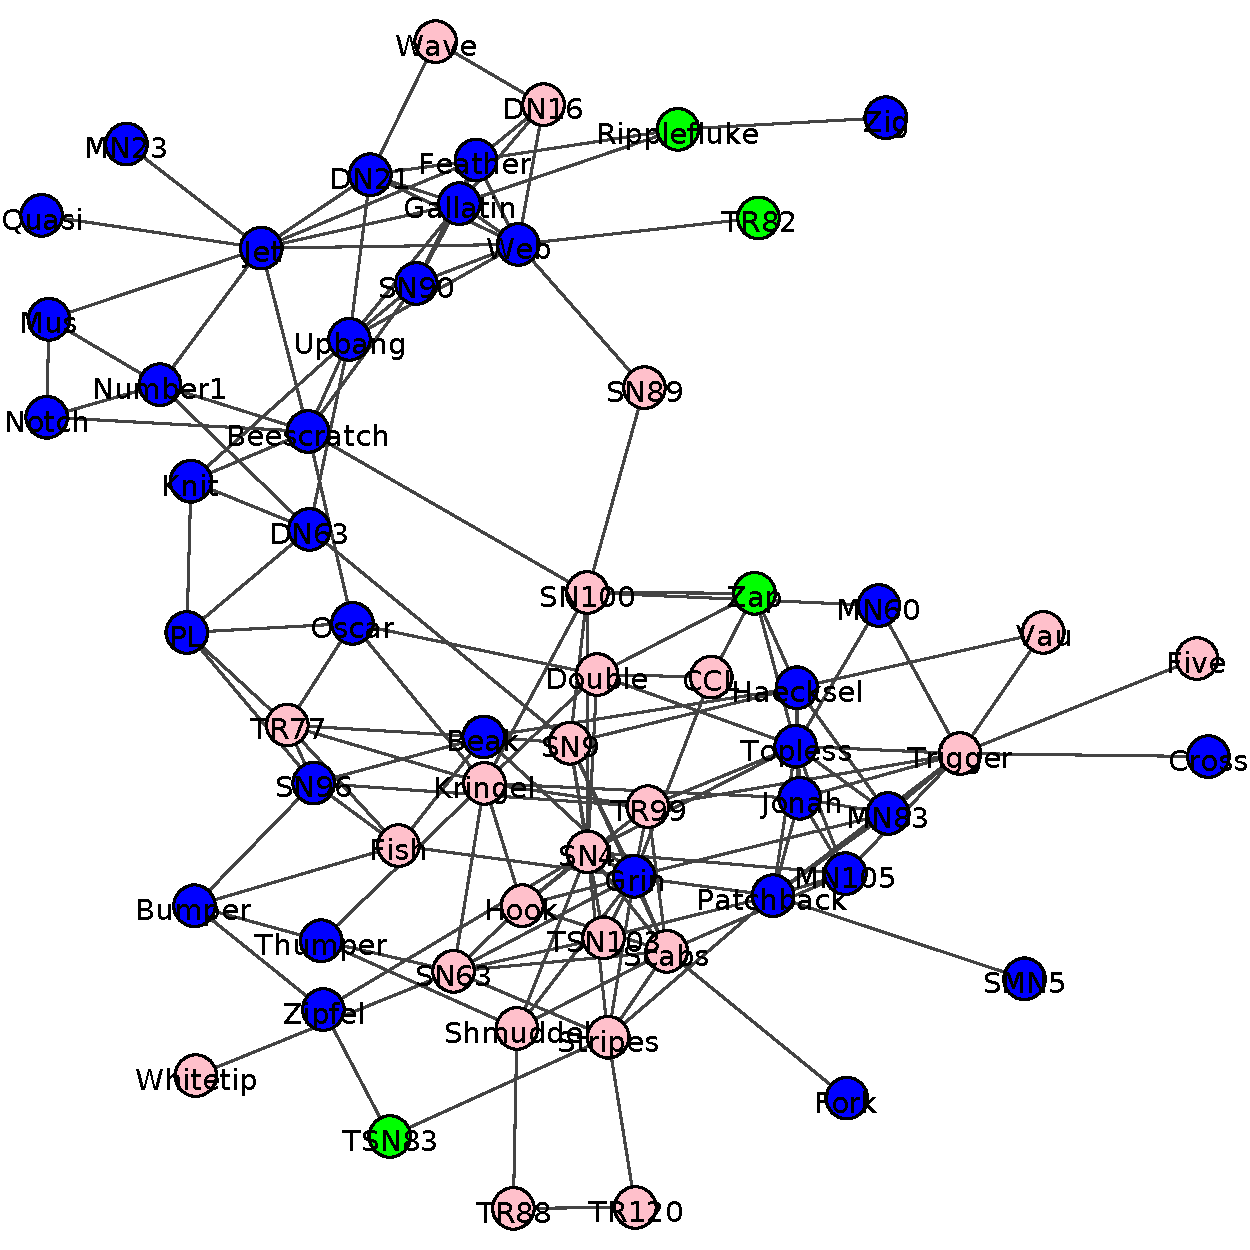
\includegraphics[scale = 0.50]{figuras/FrutRein.eps}
\caption{Fruchterman - Reingold layout. Los colores de los nodos se refieren al sexo del delfín: azul, macho; rosa, hembra; verde, sexo no indicado en el dataset.}
\label{fig:Layout_delfines}
\end{figure}

\par Exploramos diferentes layouts para visualizar la red delfines.
En la figura \ref{fig:Layout_delfines} observamos el resultado de graficar
el grafo con el Fruchterman - Reingold layout. El algoritmo para realizar este layout se basa en asignarles fuerzas de interacción ficticias a los nodos. Típicamente se basa en que los nodos ligados tengan una fuerza de atracción análoga a la fuerza de un resorte, sumado a una fuerza de repulsión entre todos los nodos, análoga a la interacción coloumbiana entre partículas cargadas idénticamente. Este tipo de layout nos permitió visualizar la existencia de dos comunas de delfines, ligadas a través de unos pocos nodos.
\par Otros layouts que nos aportarían la misma conclusión son el DrL layout y el Kamada Kawai (fig. \ref{fig:Layouts_alternativos}), que también están basados en la asignación de fuerzas ficticias. Preferimos el Fruchterman - Reingold layout, ya que los nodos aparecen mejor distribuidos, y permite una mejor visualización de la red.
\par A modo de ejemplo, incluímos otros layouts, Random, que sitúa los nodos en forma aleatoria, y Multidimensional Scaling, que se basa en una proyección matricial a un espacio de baja dimensionalidad, que no nos aportaron una buena visualización.

\begin{figure}
\centering
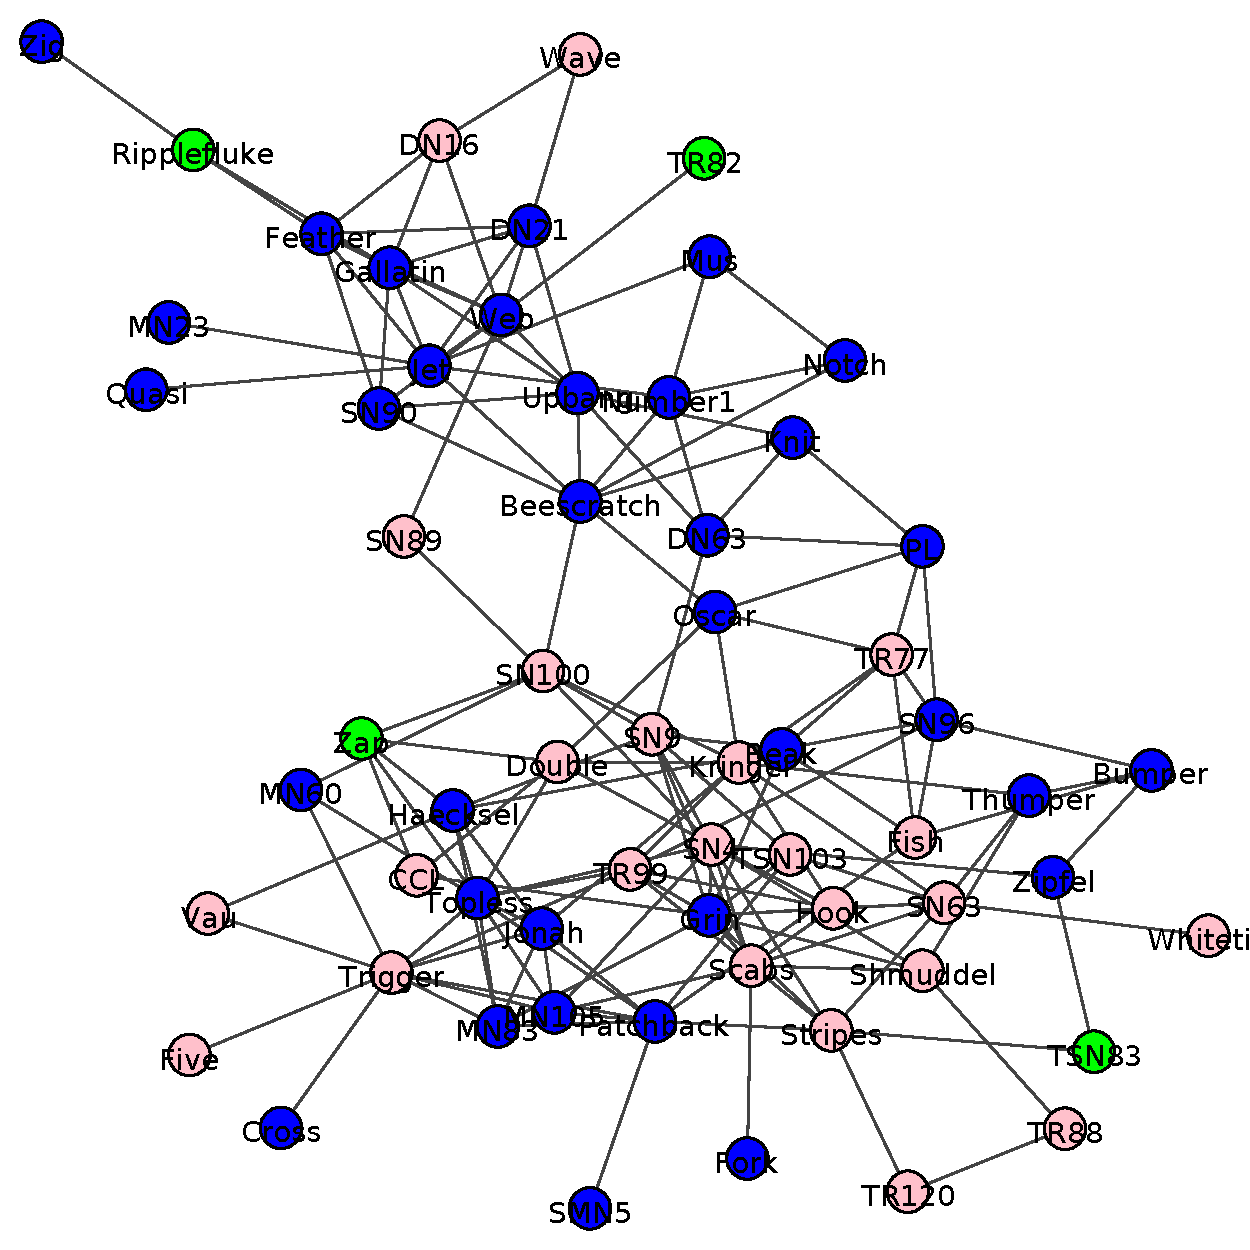
\includegraphics[scale = 0.25]{figuras/KamKaw.eps}
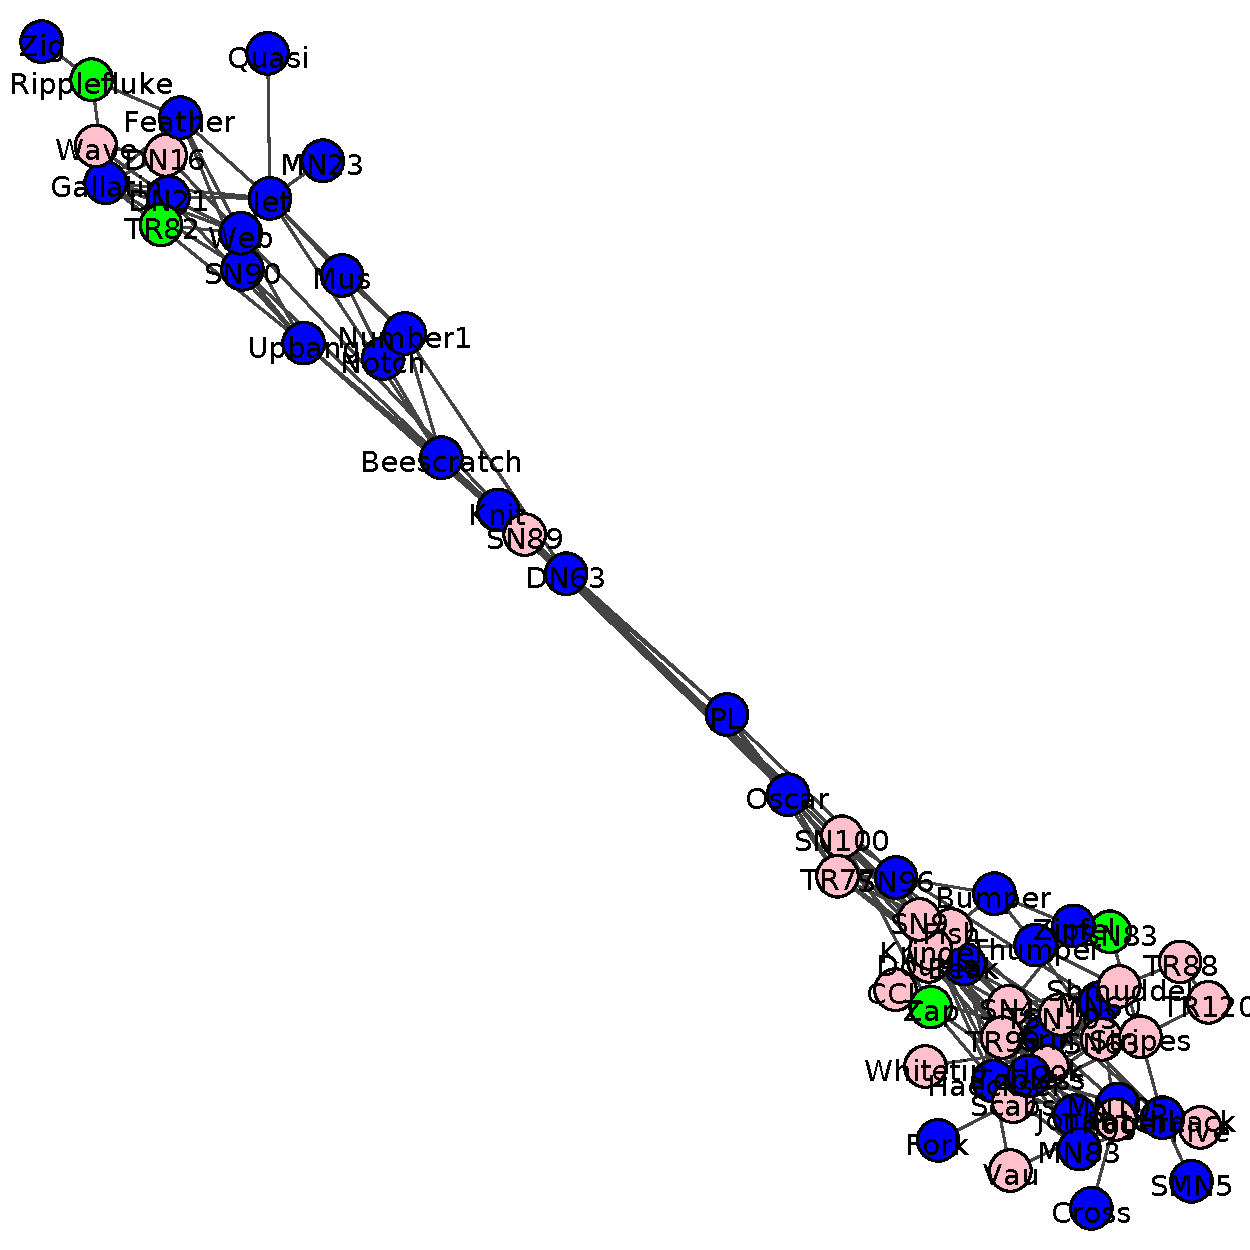
\includegraphics[scale = 0.25]{figuras/Drl.eps}
\caption{Layouts alternativos: Kamada Kawai izquierda, DrL derecha. Estos también dan la información de una red con comunas de tamaño considerable.}
\label{fig:Layout_alternativos}
\end{figure}

\begin{figure}
\centering
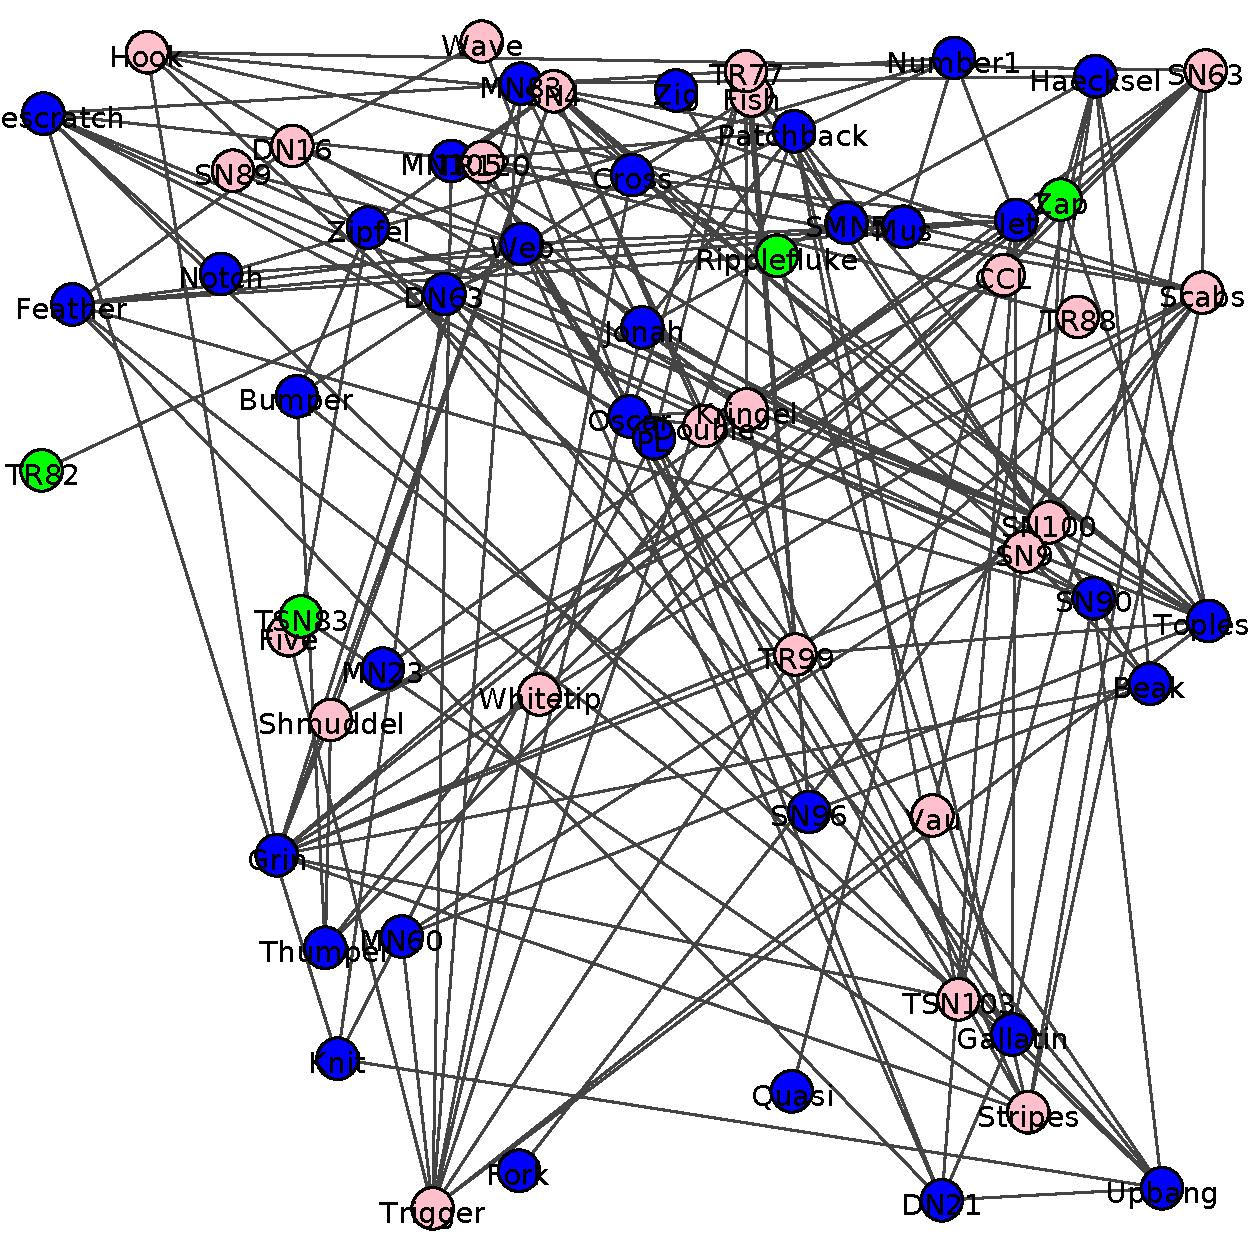
\includegraphics[scale = 0.25]{figuras/Random.eps}
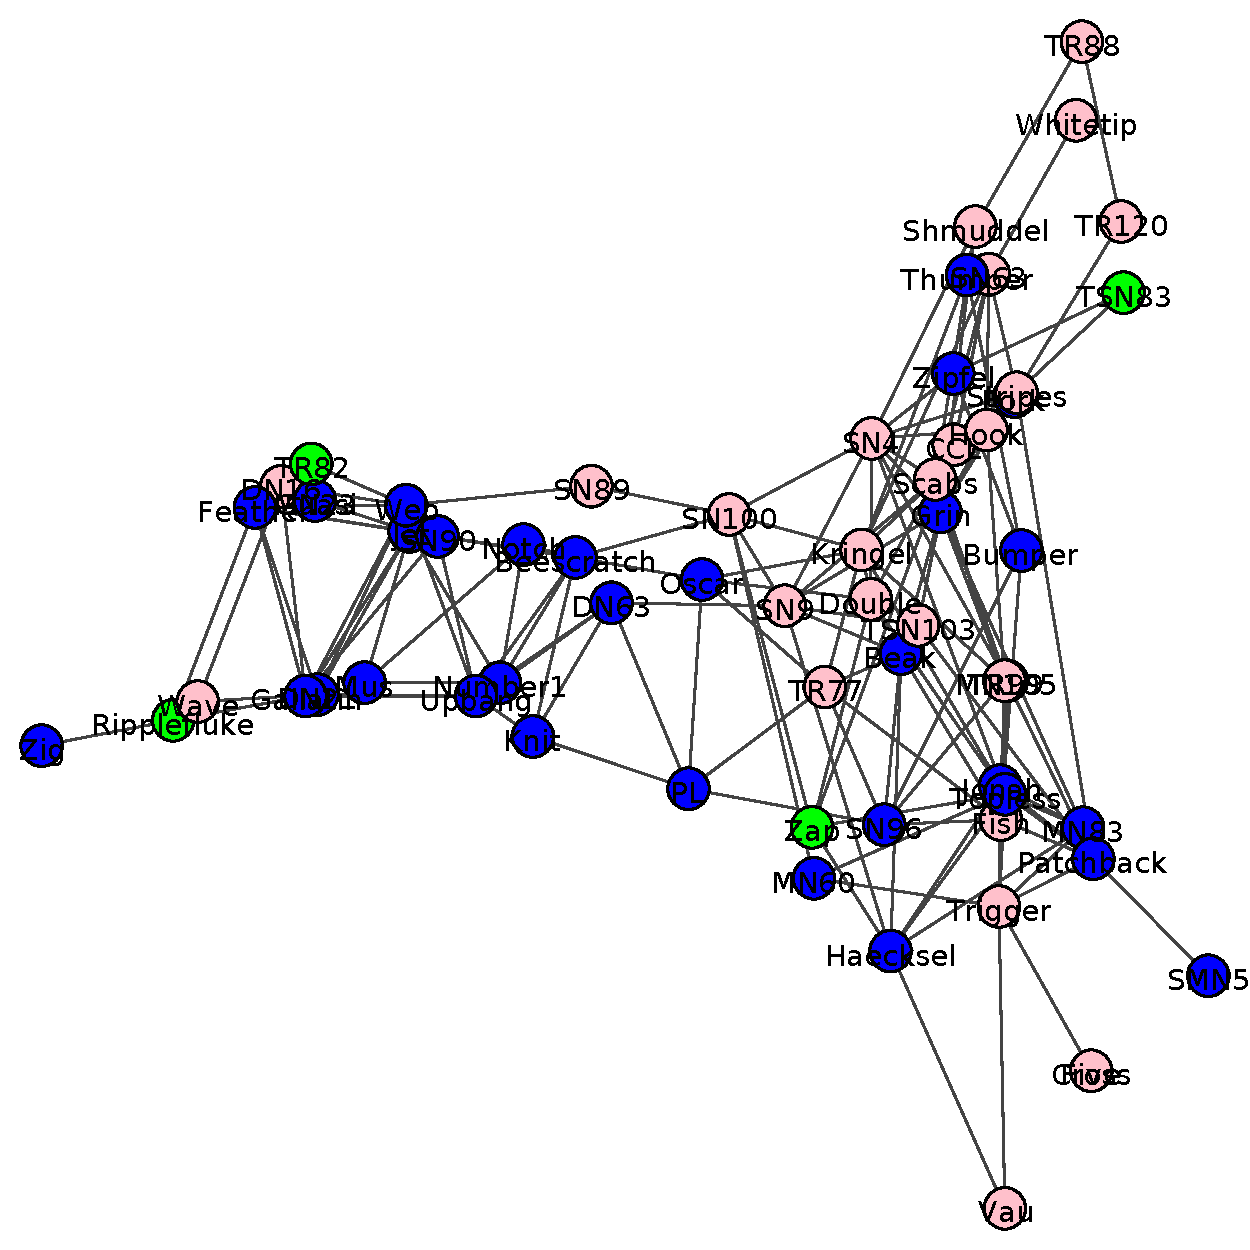
\includegraphics[scale = 0.25]{figuras/Multi.eps}
\caption{Layouts que no permiten una buena visualización del problema: Random izquierda, Multidimensional Scaling derecha.}
\label{fig:Layout_malos}
\end{figure}


\subsection{Parte b.}

\par En esta sección nos propusimos estudiar si la red es de carácter homofílica, es decir, si un dado nodo tiende a ligarse con nodos que comparten una característica con él, como es en este caso el género de los delfines. Para ello consideremos la hipótesis nula, es decir, que la asignación de género a un dado nodo es totalmente independiente de la topología de la red, y comparamos con lo presente en el dataset.
\par La metodología empleada fue la siguiente: sorteamos el género de los delfines manteniendo inalterable la topología de la red y manteniendo constante la cantidad de delfines machos, hembras, y género no específicado de la red original. Generamos $10^{6}$ realizaciones distintas, y para cada caso calculamos la cantidad de links entre delfines de distinto género (sin tomar en cuenta los links entre pares de nodos que incluya un género indefinido). El resultado es la distribución de la figura \ref{fig:Histograma}. En el mismo incluímos la cantidad de links entre géneros de la red real, que en principio se observa mucho menor que la media de la distribución.

\begin{figure}
\centering
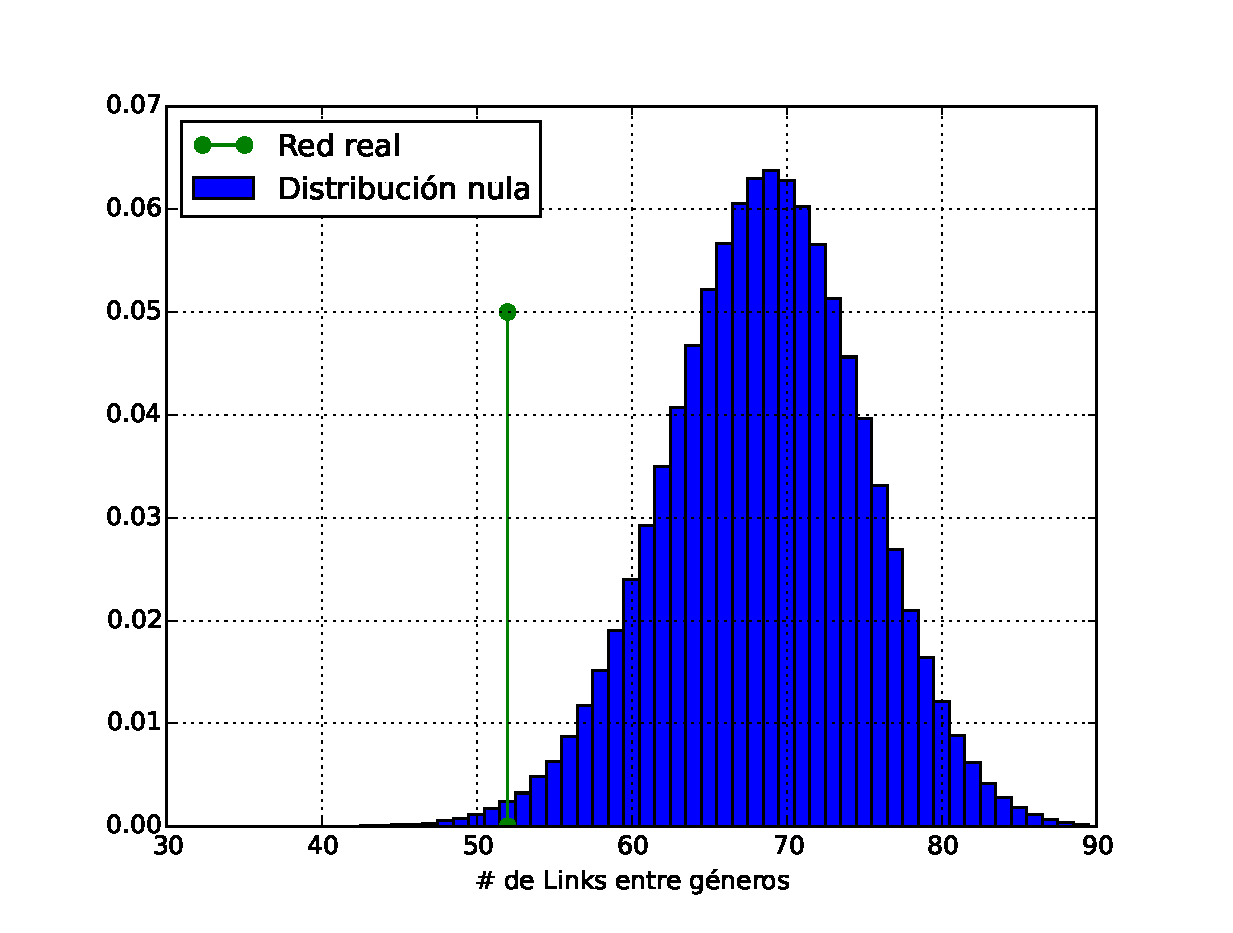
\includegraphics[scale = 0.70]{figuras/Histograma.eps}
\caption{Histograma de links entre géneros sorteando sobre la topología de la red. En verde cantidad de links entre géneros de la red actual (la altura de la barra no representa nada.)}
\label{fig:Histograma}
\end{figure}

\par Por otro lado podemos estimar la fracción de links entre géneros para una red aleatoria. Si tomamos que la probabilidad de escoger un link entre un macho y una hembra es $2 \rho_{M} \rho_{F}$, donde $\rho$ son las densidades de cada género en la red real, entonces la probabilidad de la tomar $m$ links de esta característica es:
\begin{equation}
	P(m) = {N' \choose m} (2 \rho_{M} \rho_{F})^{m} (1 - 2 \rho_{M} \rho_{F})^{N' - m}
\end{equation}
donde $N'$ es $N(N-1)/2$, el número total de links que se pueden formar en una red de $N$ nodos. Con esta distribución, el valor medio de links y la desviación standard resultan:
\begin{align*}
	<m> & = 2 N' \rho_{M} \rho_{F} \\
	std(m) & = (2 N' \rho_{M} \rho_{F} (1 - 2 \rho_{M} \rho_{F}))^{1/2}\\
\end{align*}
Por lo tanto, la fracción de links ($<m>/N'$) para las densidades de género actuales, estimado mediante la ecuación anterior, y el resultado del sorteo considerando la hipótesis nula resultan:

\begin{align*}
	(\frac{<m>}{N'}){estimado} & = 0.43 \pm 0.01 \\
	(\frac{<m>}{N'})_{hip.nula} & = 0.43 \pm 0.04
\end{align*}
donde el último valor se obtuvo dividiendo $<m> = 68 \pm 7$ (obtenido del sorteo) y $N' = 159$, que es el número de links totales de la red real). Observamos que el valor estimado y el obtenido sorteando al azar el género de los delfines coindicen.
\par Como puede deducirse de la figura \ref{fig:Histograma}, la probabilidad de que se obtengan la cantidad de links entre géneros de la red actual dada la hipótesis nula es menor a $0.005$, por lo que descartamos la hipótesis nula, y concluimos que la red es homofílica: la cantidad de links entre géneros es mucho menor que el valor esperado si la distribución de géneros fuera aleatoria, lo que implica que hay más cantidad de enlaces entre delfines del mismo sexo, y además la probabilidad que el valor actual se dé por simple aleatoriedad es muy baja.

\subsection{Parte c.}

\par Como último punto, proponemos un método para dividir la red en dos componentes de tamaño comparable. Debido a que suponenmos que la red se constituye principalmente de dos comunas ligadas por pocos nodos, consideramos que el cálculo del betweenness no dará información sobre dichos nodos. El betweenness tiene en cuenta la cantidad de caminos cortos que pasan por un dado nodo. Su remoción implicaría un aumento en la distancia entre nodos. Formalmente, el betweenness de un nodo se calcula como:
\begin{equation}
	Bet(i) = \sum_{j,k} \frac{b_{jik}}{b_{jk}}
\end{equation}
donde $b_{jk}$ es número de caminos cortos que van desde $j$ hasta $k$, y $b_{jik}$ es el número de caminos cortos que van desde $j$ hasta $k$, que pasan por $i$.
\par Removiendo los nodos con mayor betweenness, basta remover 4 nodos para descomponer la red en dos conjuntos no conexos, como puede observarse en la figura \ref{fig:Betweenness}. Si lo comparamos con el caso de remover nodos al azar sin más criterio, es muy díficil obtener este resultado. En la figura \ref{fig:Comparacion}, mostramos el tamaño del componente conectado más grande del sistema a medida que removemos nodos con los dos métodos. Podemos observar que siguiendo el criterio de remover siempre el nodo con mayor betweenness, el tamaño del componente más grande tiene caídas abruptas, lo que indica una partición en el grafo de componentes de tamaño considerable. Sin embargo, al remover al azar, se observa que el componente más grande va disminuyendo su tamaño de forma suave con la remoción de cada nodo particular. 

\begin{figure}
\centering
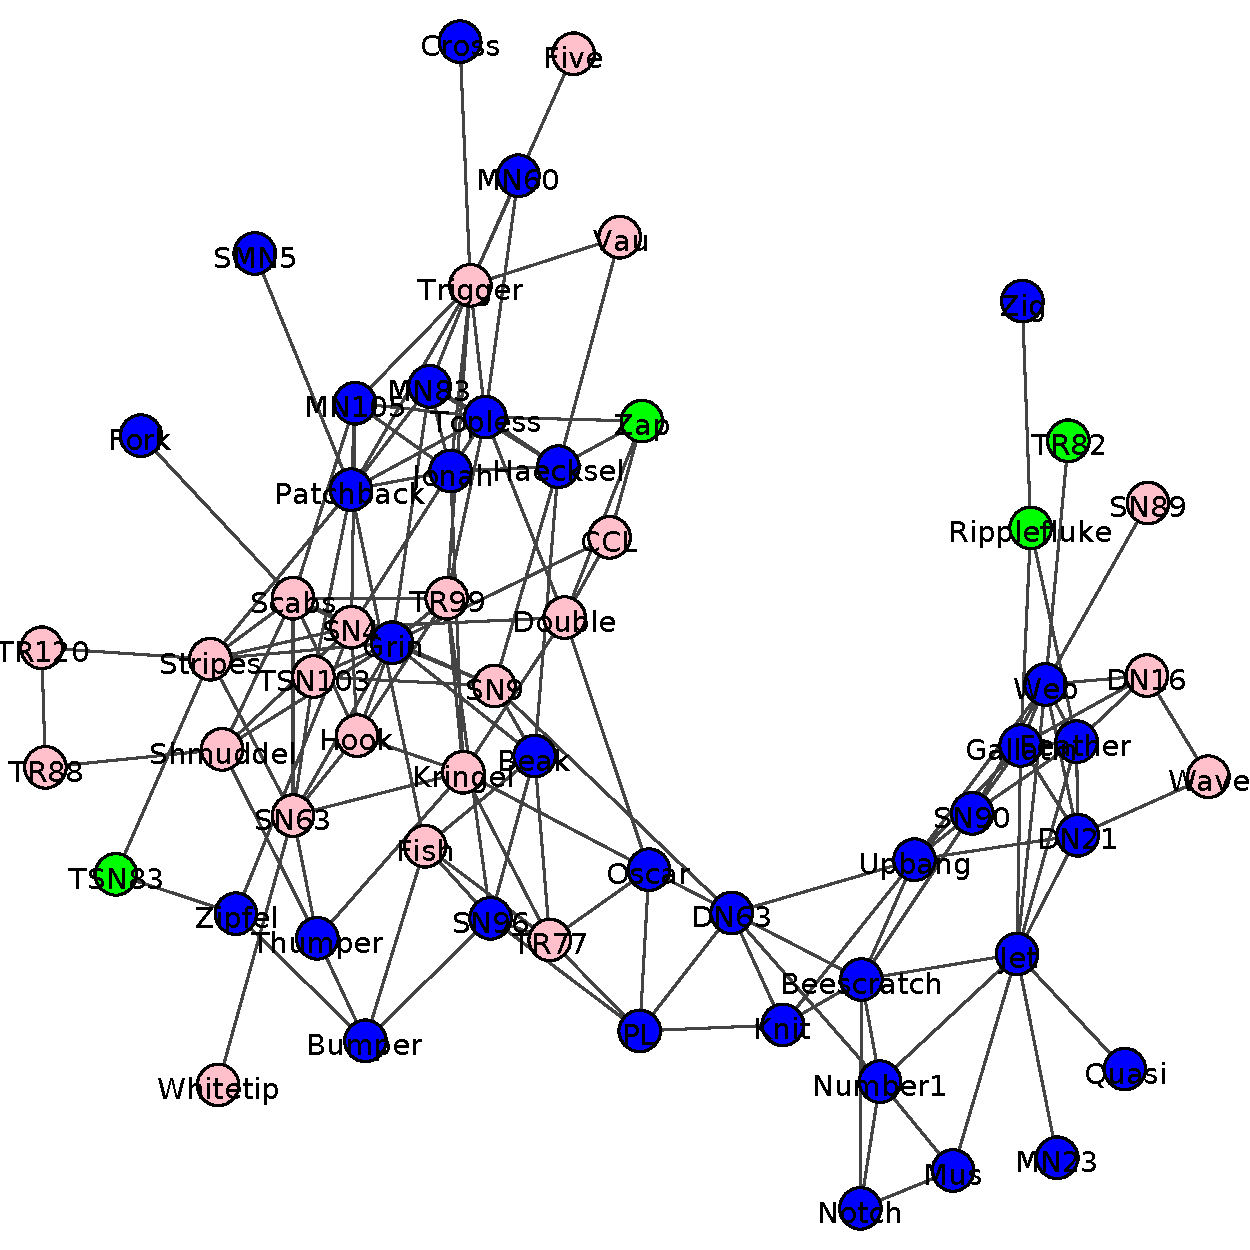
\includegraphics[scale = 0.28]{figuras/Parte_c0} 
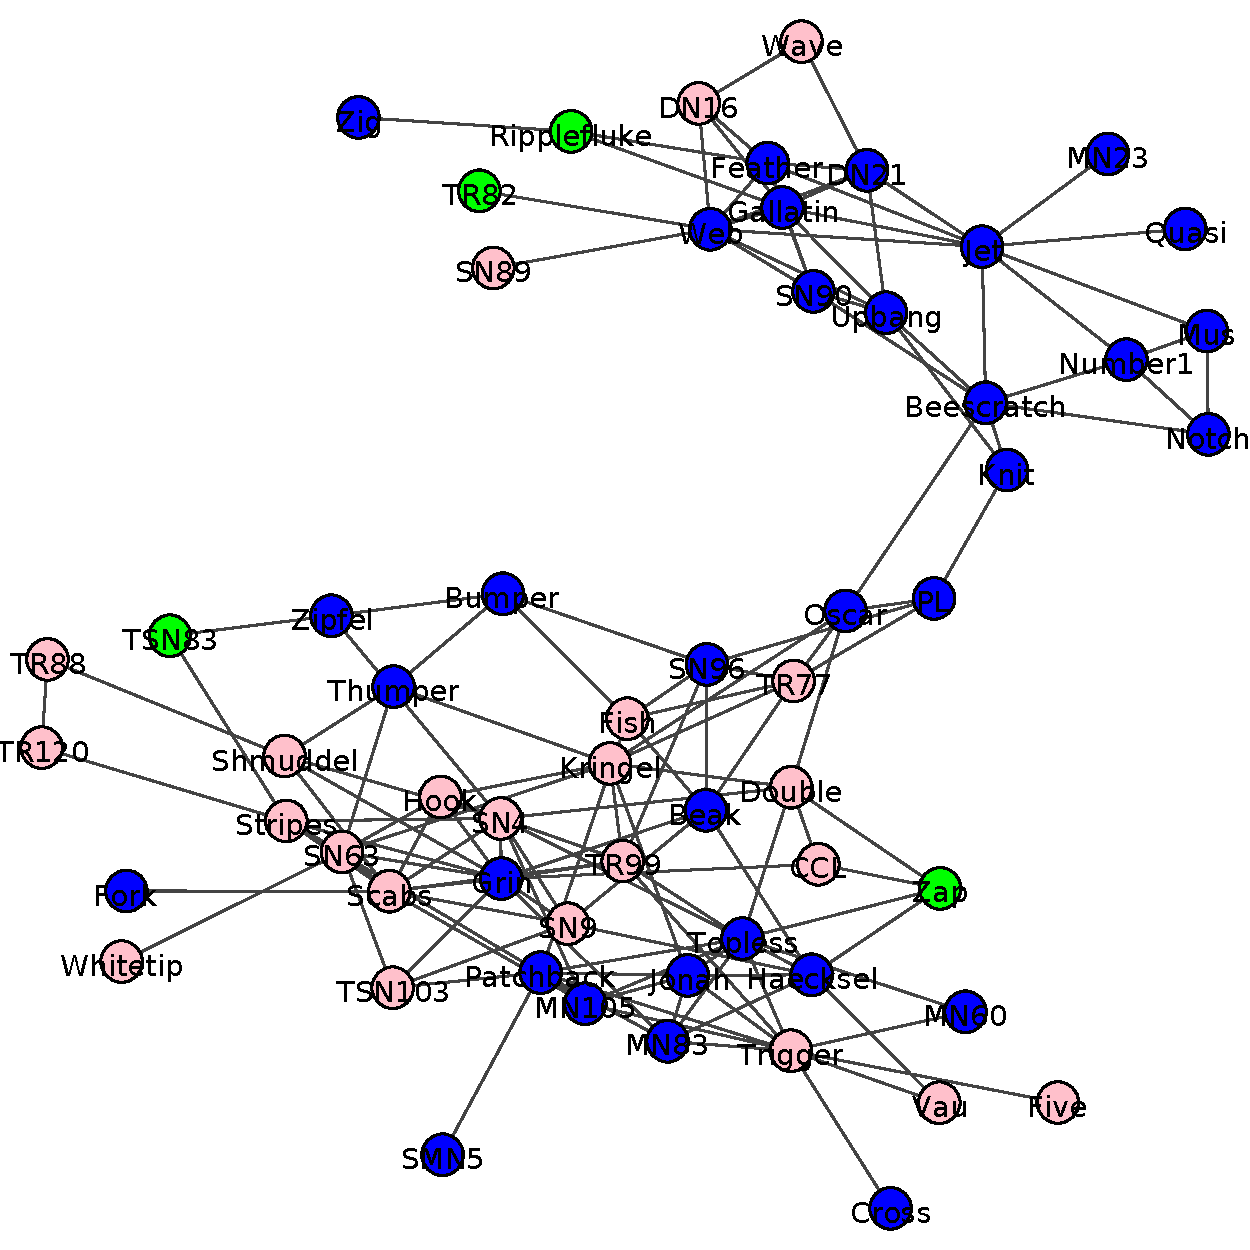
\includegraphics[scale = 0.28]{figuras/Parte_c1} \\
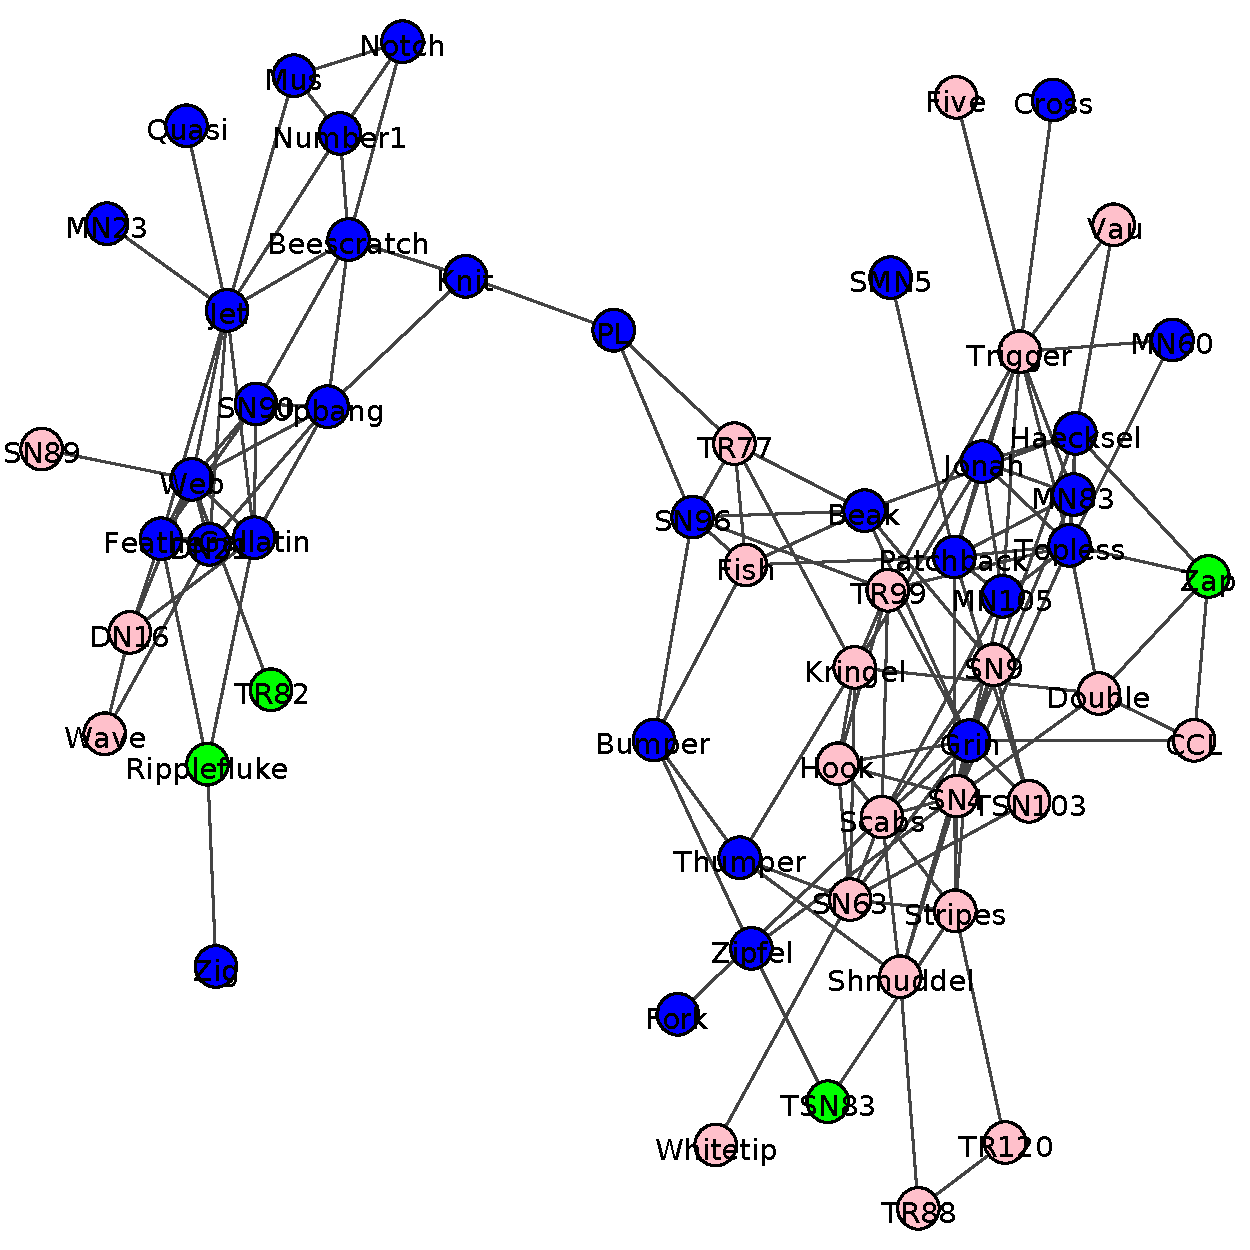
\includegraphics[scale = 0.28]{figuras/Parte_c2} 
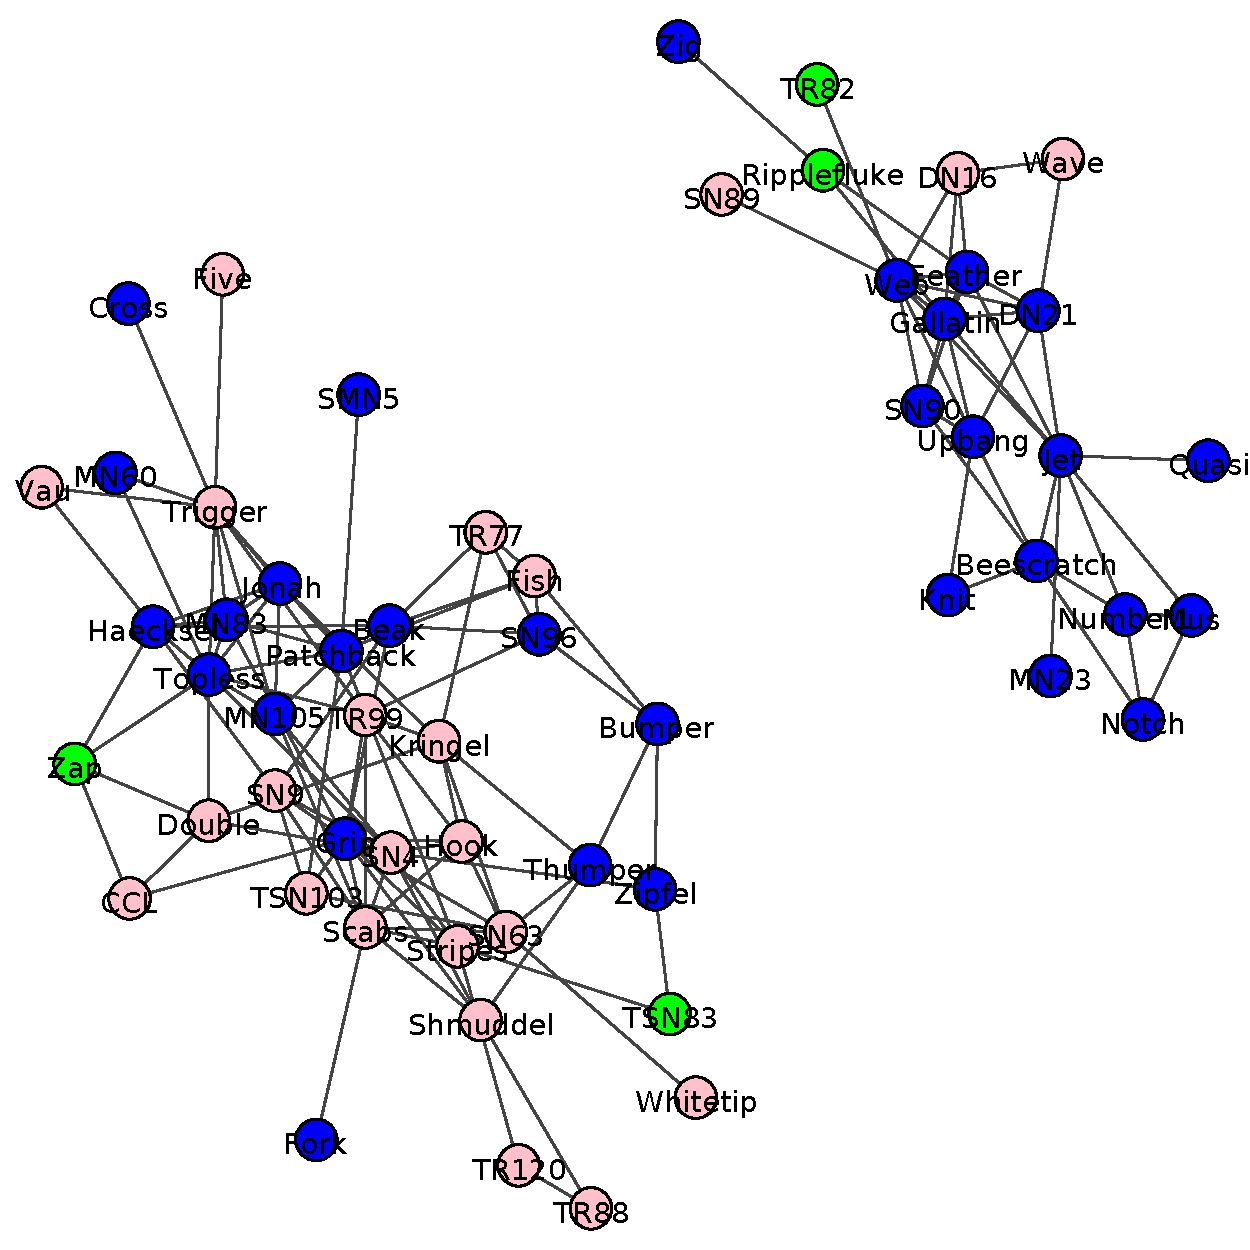
\includegraphics[scale = 0.28]{figuras/Parte_c3} 
\caption{Layout de la red al remover el nodo con mayor betweenness: remoción de izquierda a derecha, y de arriba hacia abajo. Con solo remover 4 nodos, la red se descompone en dos subgrafos de tamaño comparable.}
\label{fig:Betweenness}
\end{figure}

\begin{figure}
\centering
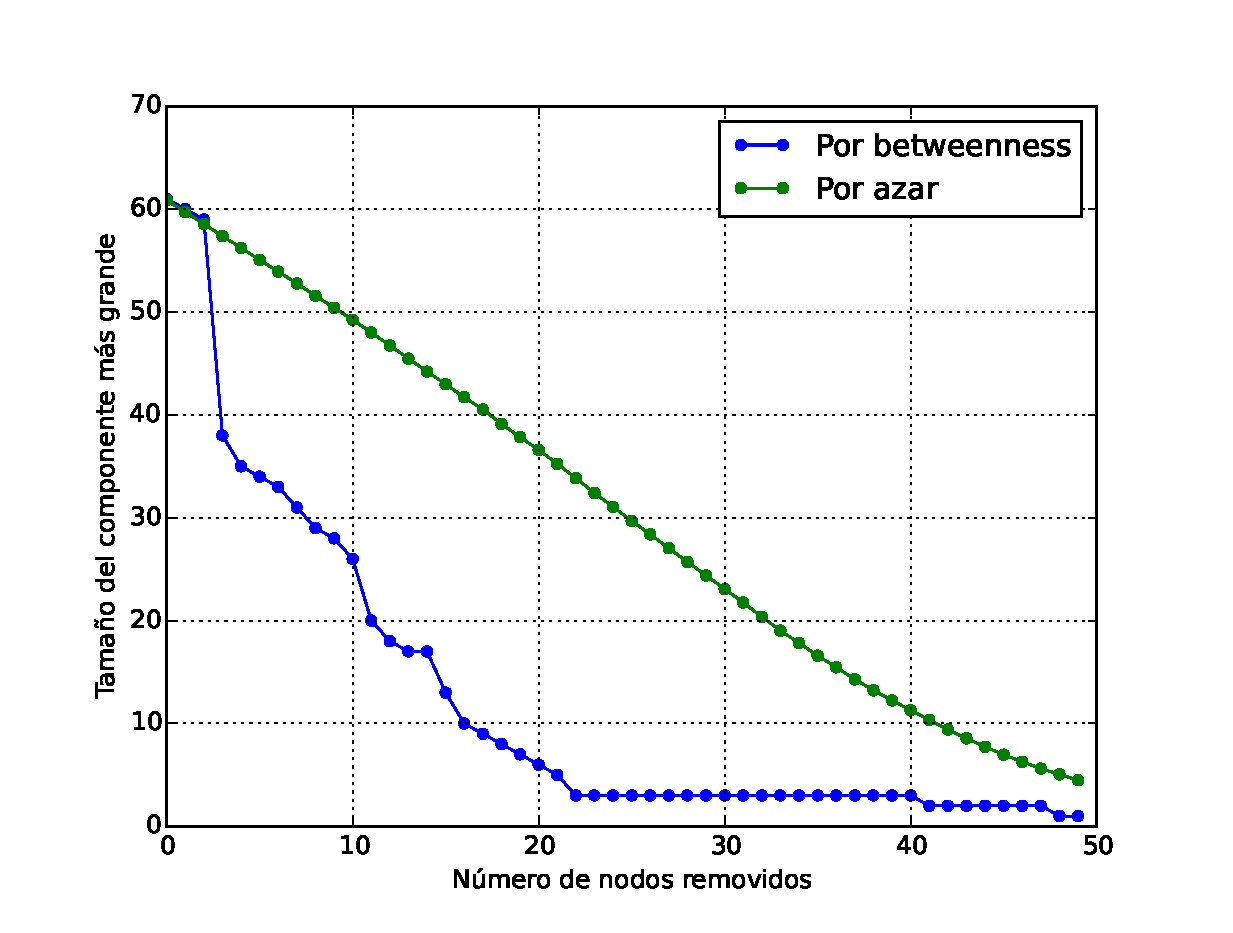
\includegraphics[scale = 0.60]{figuras/Nodos_removidos} 
\caption{Tamaño del componente más grande a medida que se remueven nodos según betweenness, o al azar, respectivamente. Observar la caída abrupta al remover 4 nodos de mayor betweenness. La curva correspondiente a la forma azarosa es un promedio de 1000 configuraciones.}
\label{fig:Comparacion}
\end{figure}


%    ../ej_03/informe.tex

%    \section{Ejercicio 4}
La asortatividad/homofilia es la tendencia de un nodo, de una red, se conecte con otros 
de caracteristicas similares, esto en terminos mathematicos es evaluar la correlaci\'on
de links entre nodos del mismo tipo \citep{newman2003}. Esta propiedad tiende a ser caracteristica 
para tipos de redes distintas: En redes de amistad por ejemplo se tiende a hacer uniones entre
nodos \textit{parecidos}, mientras que en redes biologicas, los \textit{hubs} tienes a evadirse 
entre ellos y asociarse con nodos de menor grado \citep{newman,barabasi}. 

En este ejercicio se plantea evaluar la asortatividad de cuatro redes (dos sociales y dos biol\'ogicas) a trav\'es
de dos m\'etodos distintos: Mediante la estimaci\'on de la correlaci\'on de grado a partir del grado medio del
vecindario de un nodo \citep{barabasi}; y a trav\'es del Coeficiente de Correlaci\'on de Grado propuesto por Newman
\citep{newman2003,newman}.

\subsection{Consideraciones generales}
\begin{figure}[!ht]
    \centering
    \begin{subfigure}[b]{0.30\columnwidth}
        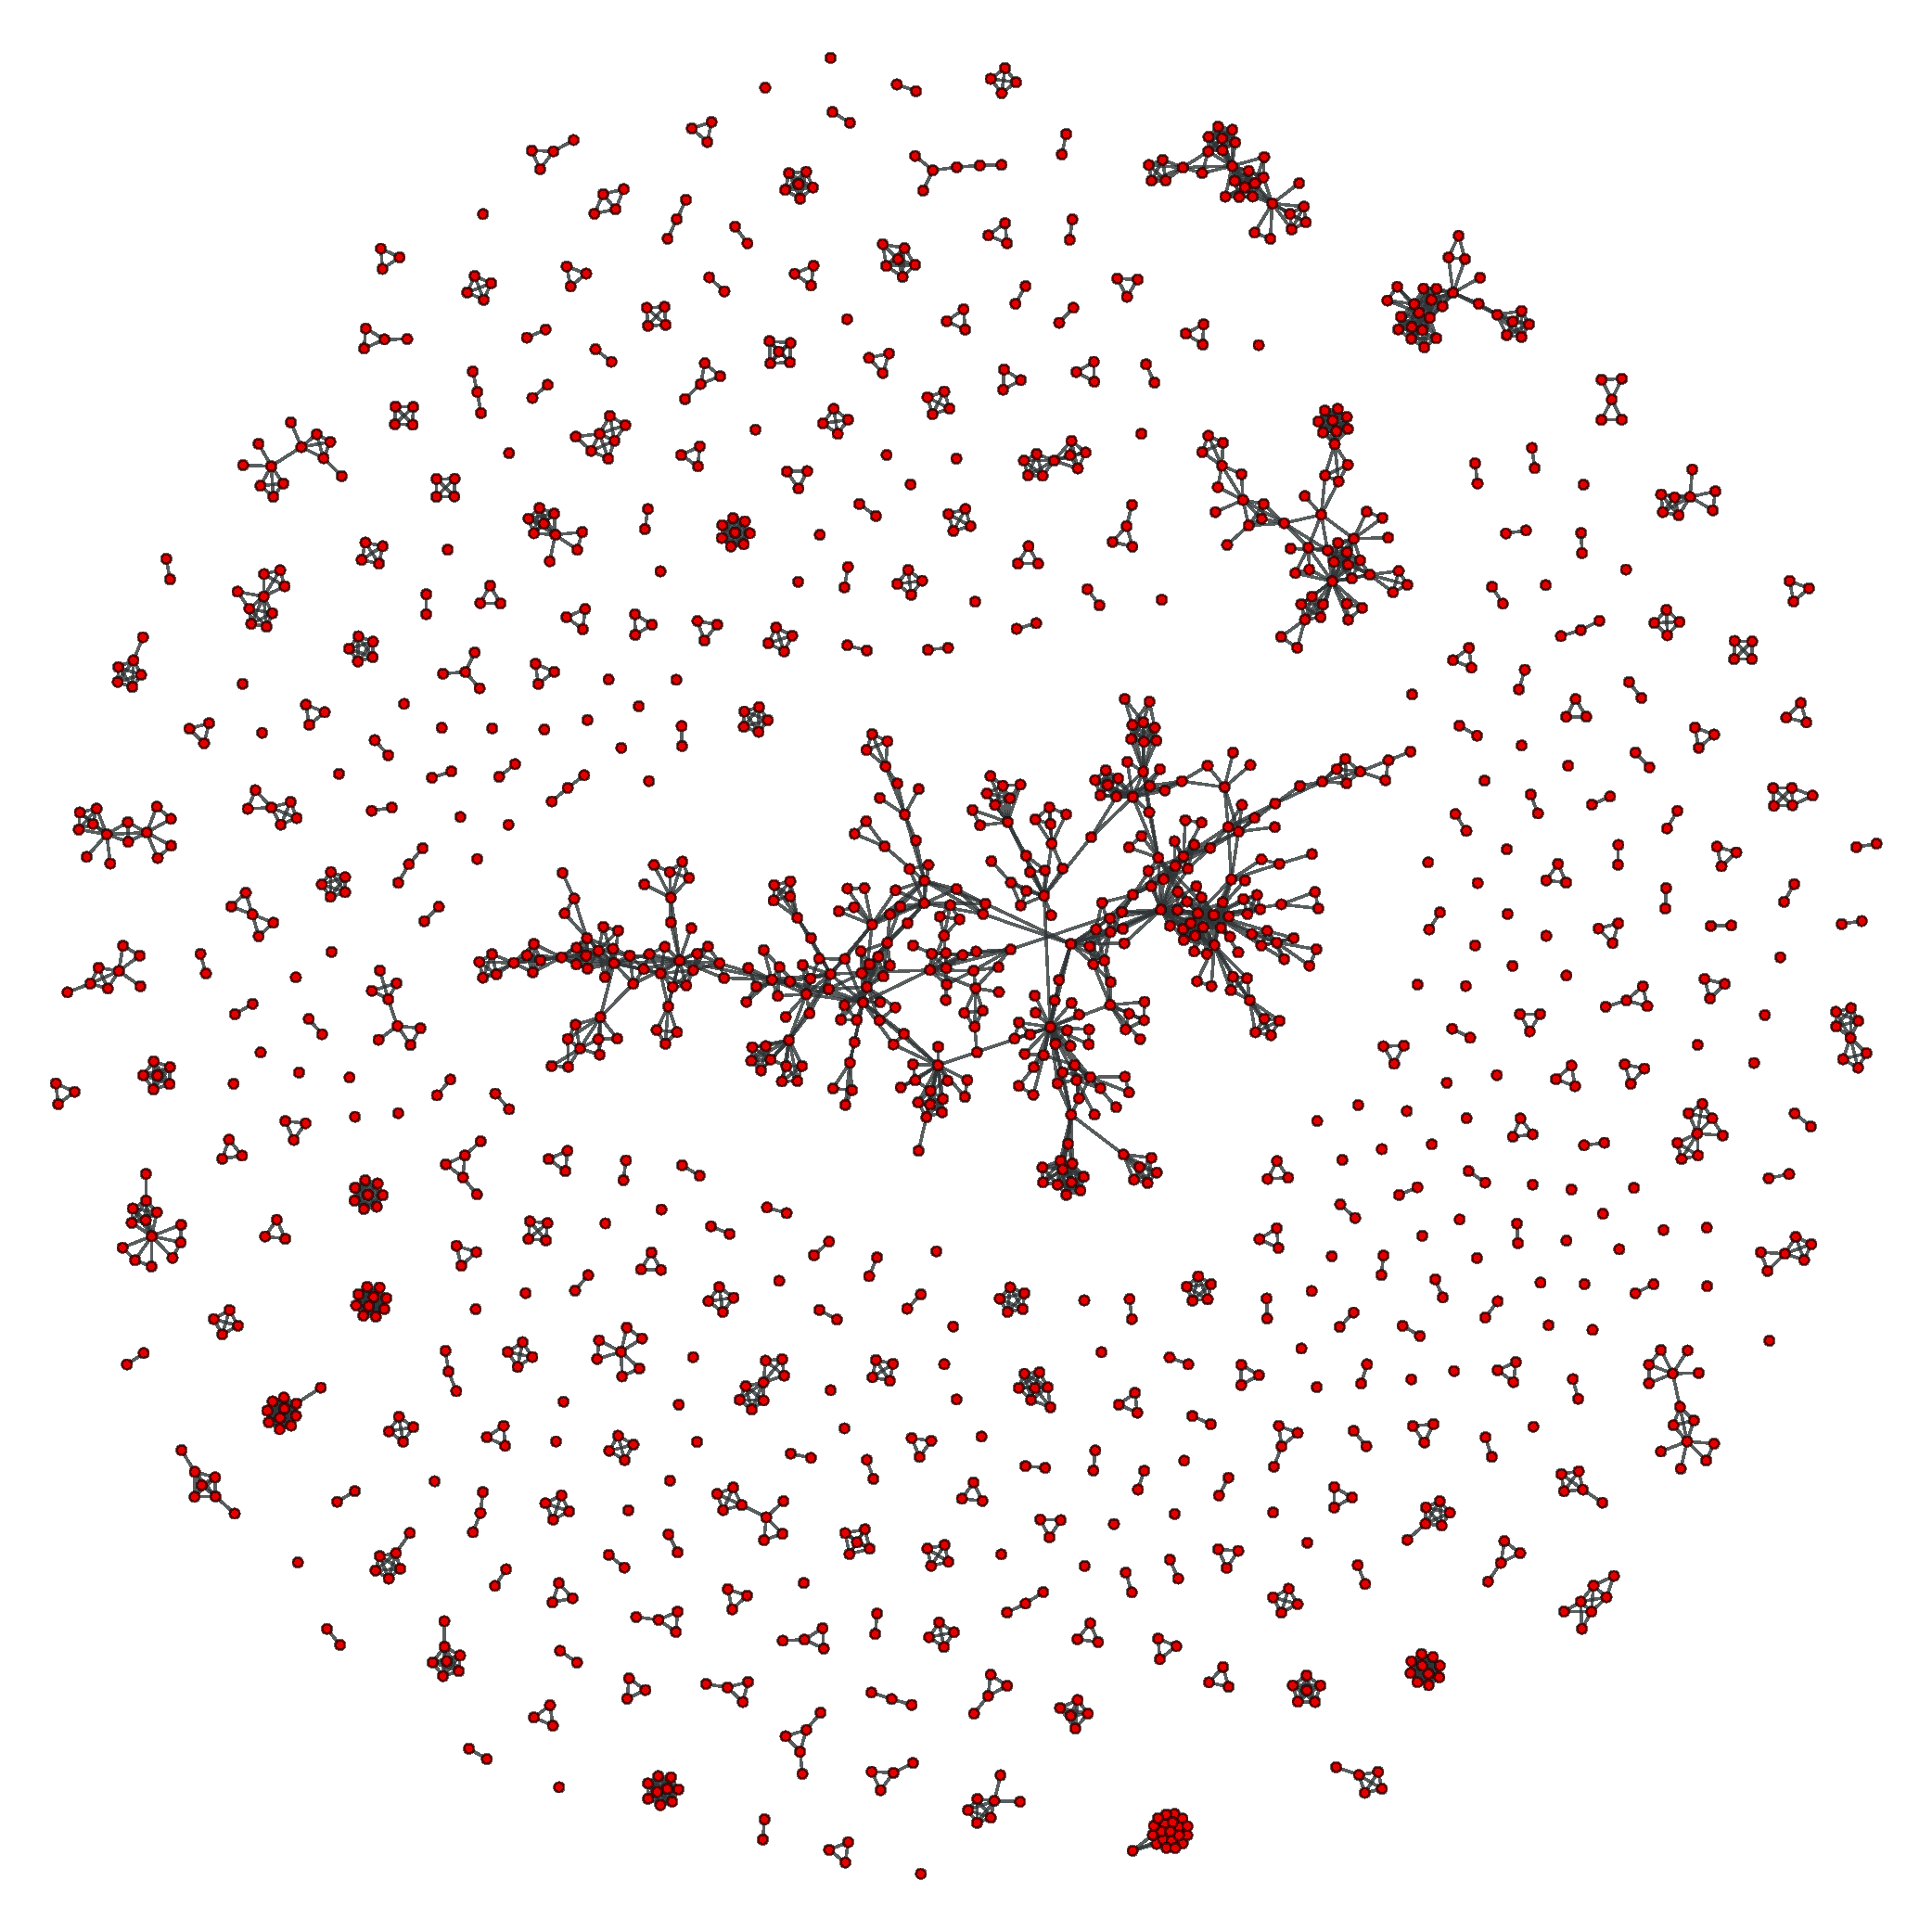
\includegraphics[width=\textwidth]{./schemes/netscience-gml.pdf}
        \caption{\label{fig4:NETSCIENCE}NETSCIENCE}
    \end{subfigure}
    \begin{subfigure}[b]{0.30\columnwidth}
        \includegraphics[width=\textwidth]{./schemes/as-22july06-gml.pdf}
        \caption{\label{fig4:INTERNET}INTERNET}
    \end{subfigure}
    \\
    \begin{subfigure}[b]{0.30\columnwidth}
        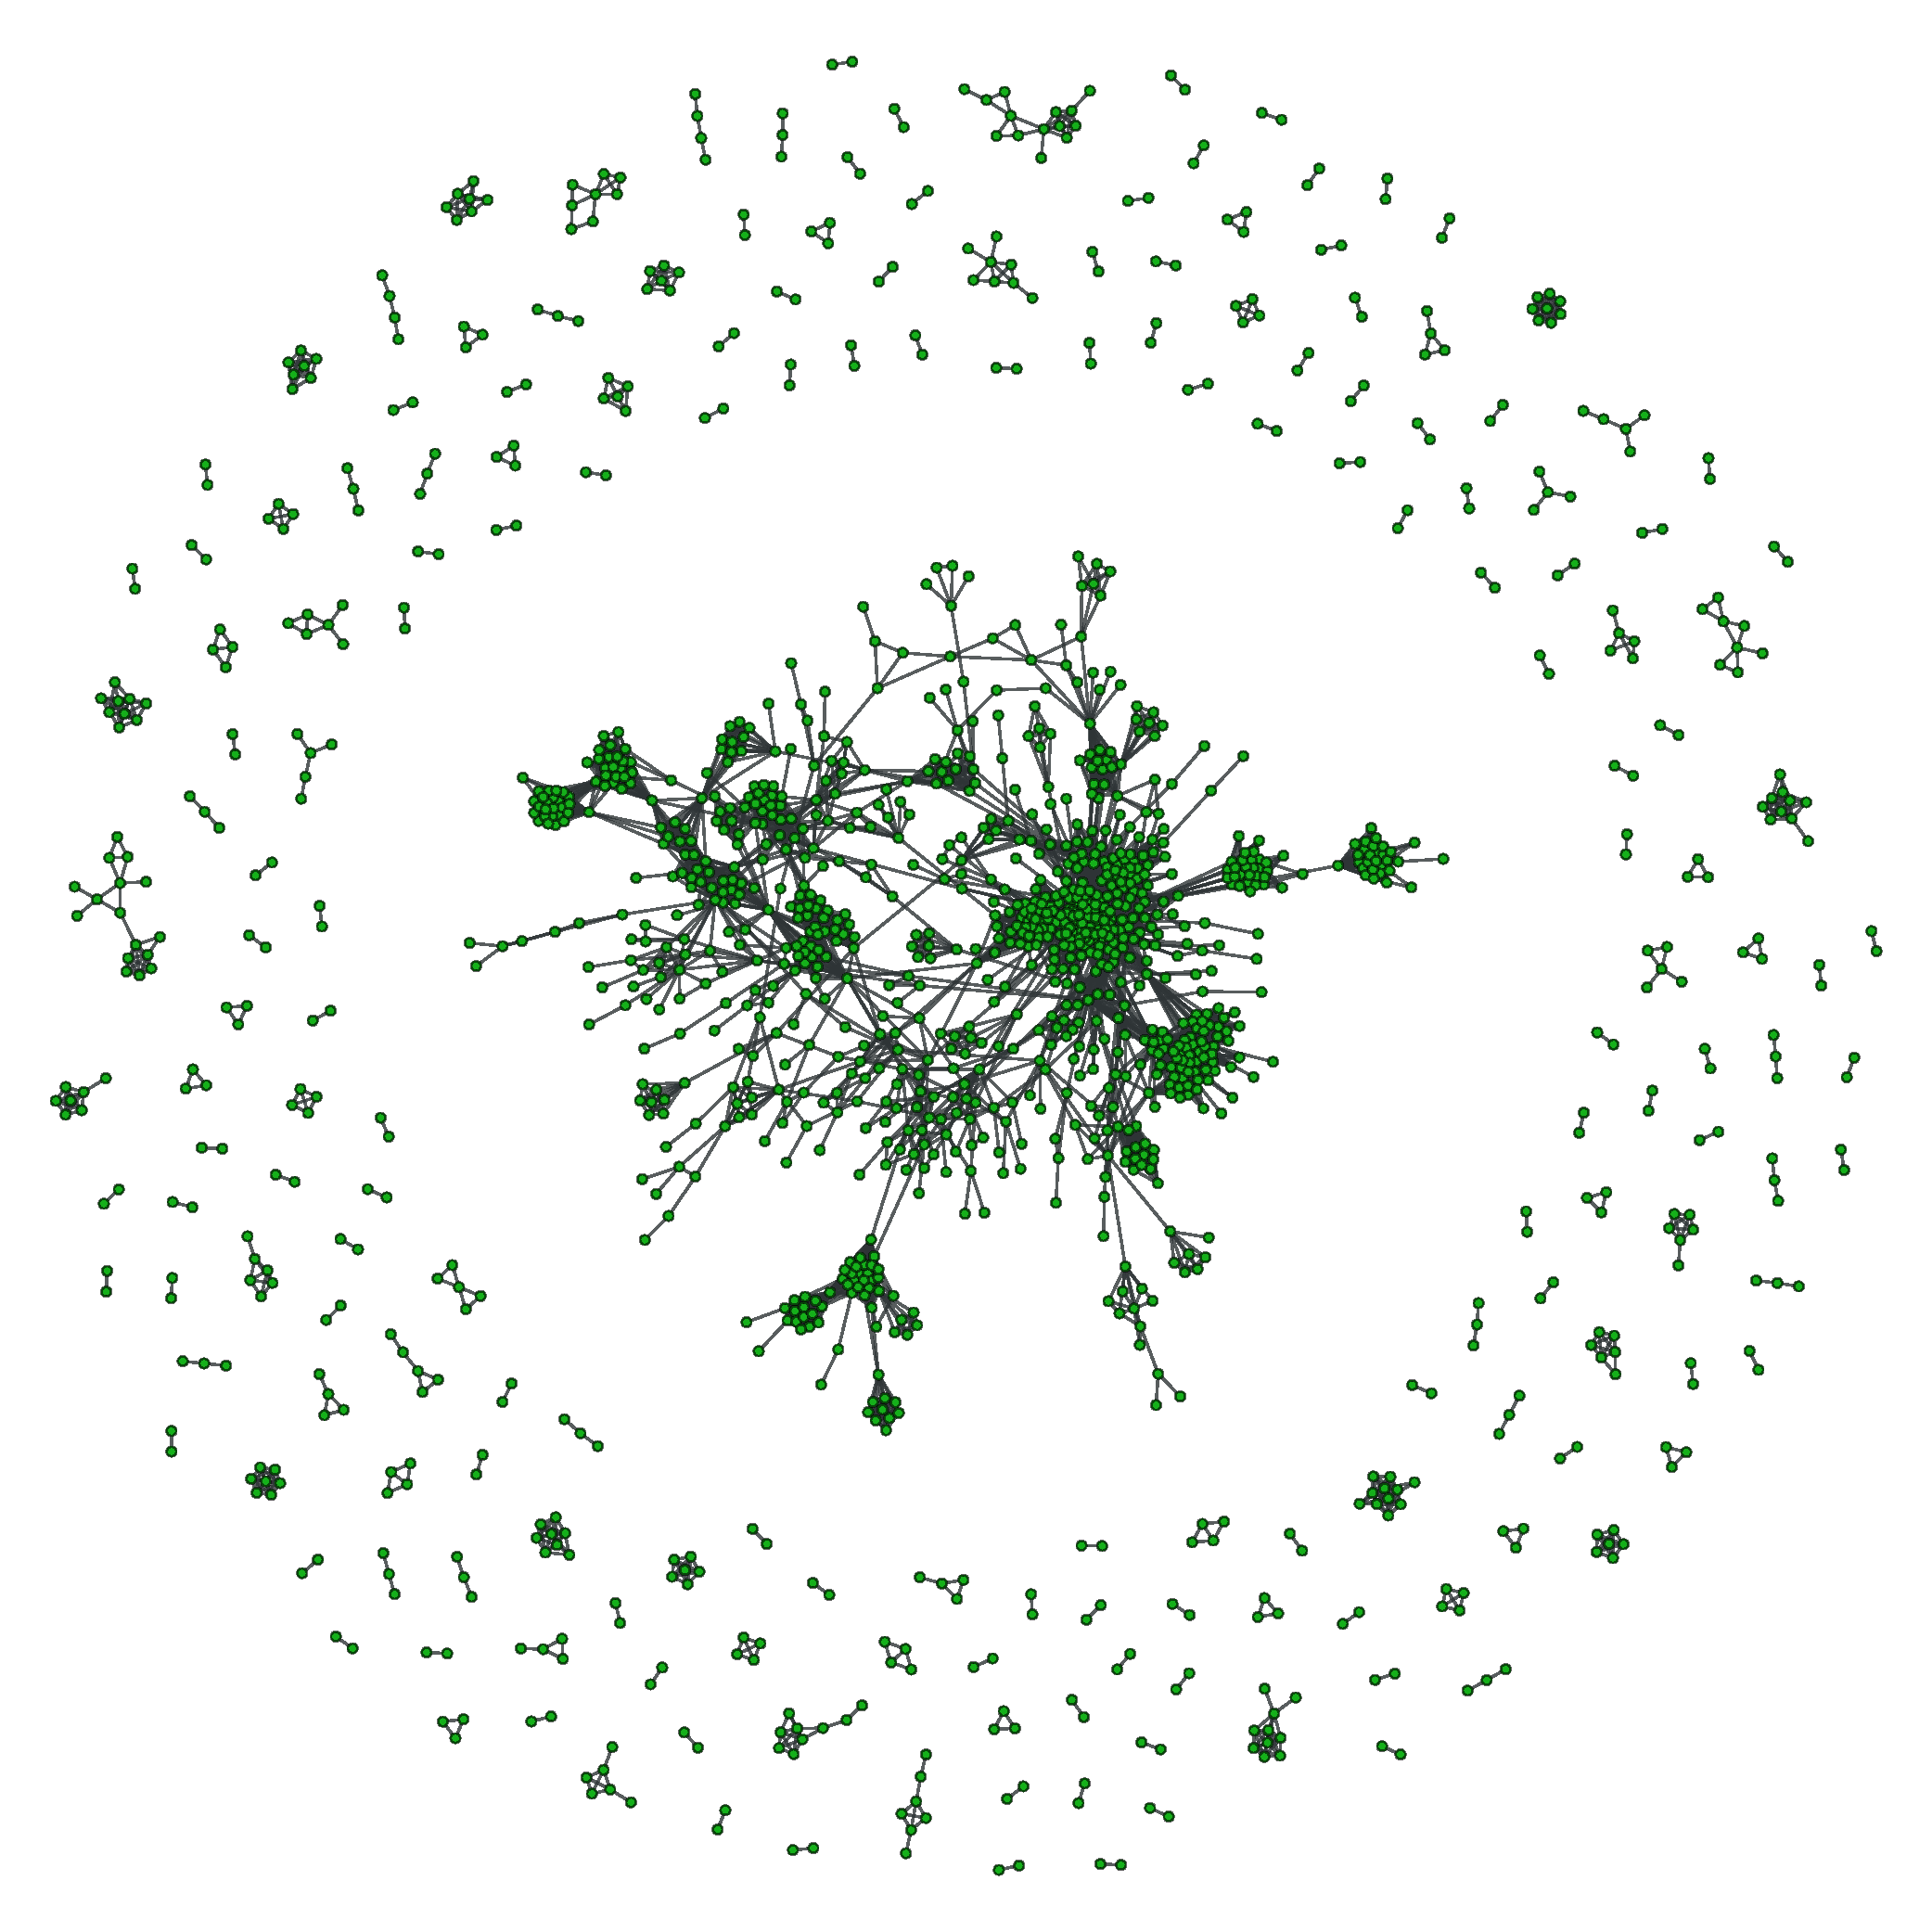
\includegraphics[width=\textwidth]{./schemes/yeast_AP-MS-txt.pdf}
        \caption{\label{fig4:ap_ms} AP-MS}
    \end{subfigure}
    \begin{subfigure}[b]{0.30\columnwidth}
        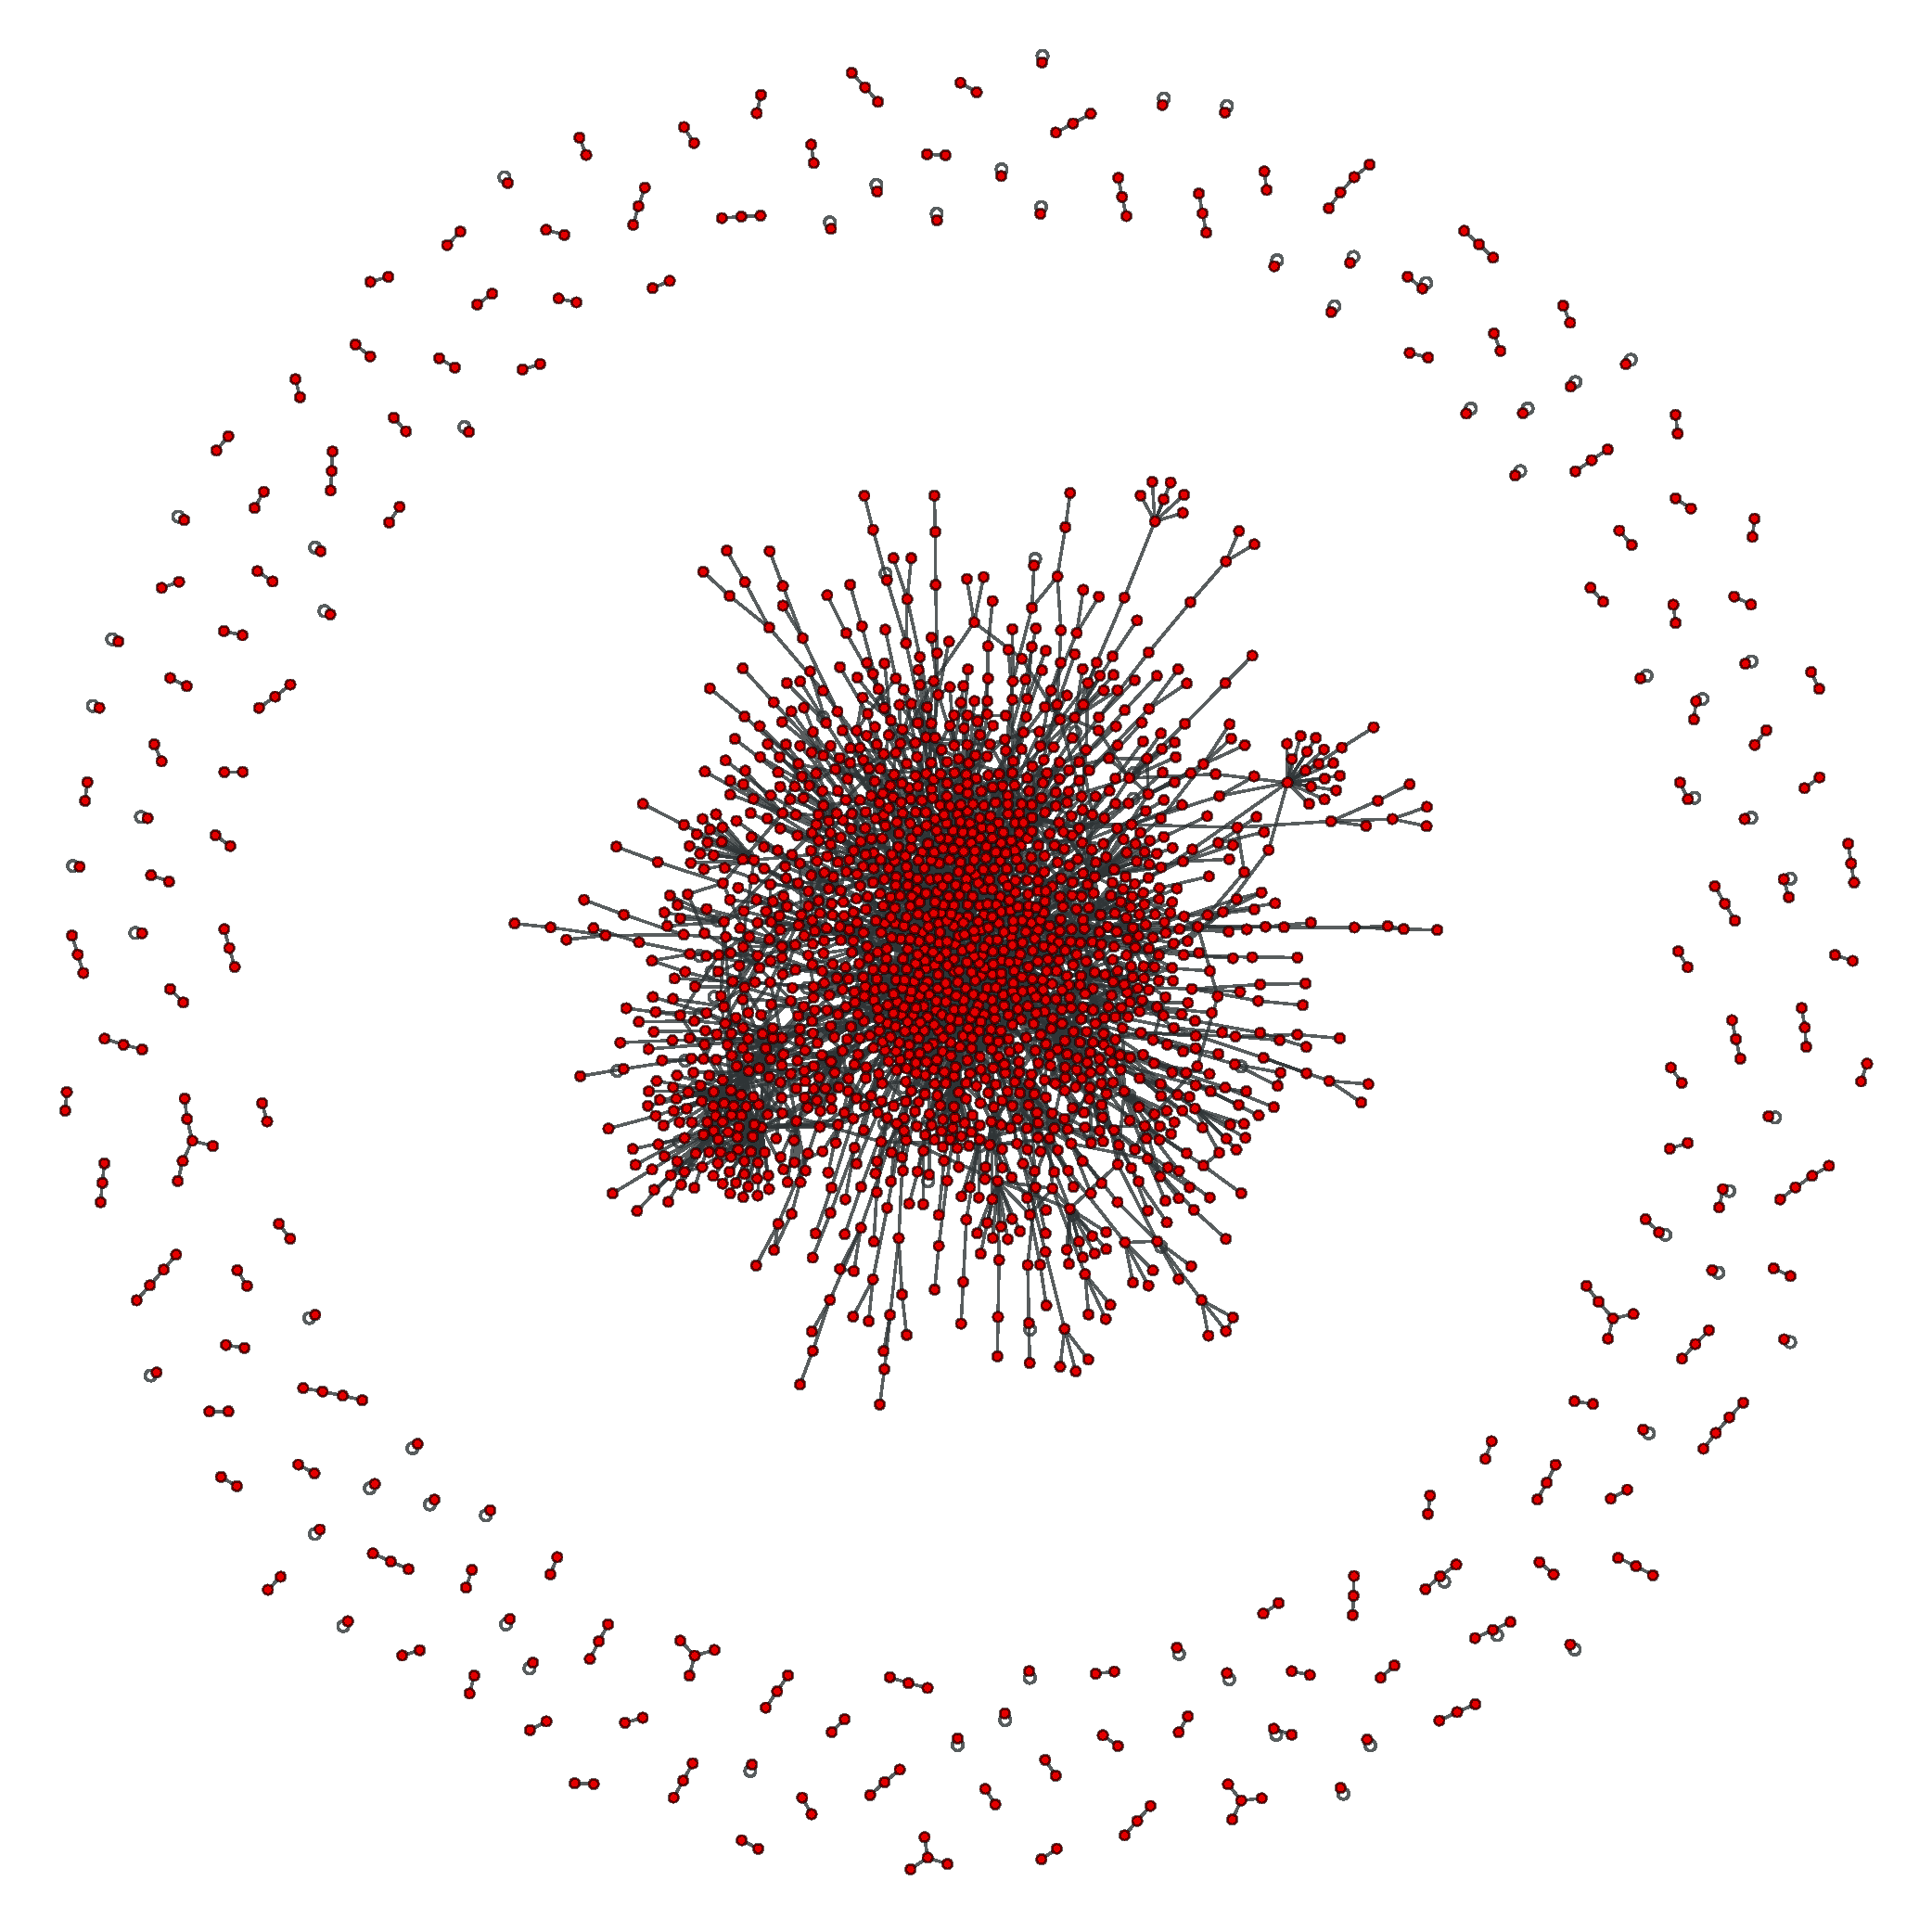
\includegraphics[width=\textwidth]{./schemes/yeast_Y2H-txt.pdf}
        \caption{\label{fig4:y2h} Y2H}
    \end{subfigure}
    \caption{\label{fig4:grafos}\textit{Layout} SFDP para cada red estudiada \\
    (script \texttt{plot.py~<archivo>\quad-f <fmt>}).}
\end{figure}
Consideremos las redes de colaboraciones cientificas (NETSCIENCE), red de internet (INTERNET) y dos redes de levadura analizadas 
en el ejercicio 1 (AP-MS y Y2H), las cuales son mostradas en la figura \ref{fig4:grafos}.


Un m\'etodo alternativo para 
evaluar asortividad es analizar la matriz de correlaci\'on entre grados (\textit{mixing matrix}) la cual se presenta en
la figura \ref{fig4:mix}.


\begin{figure}[!ht]
    \centering
    \begin{subfigure}[b]{0.45\columnwidth}
        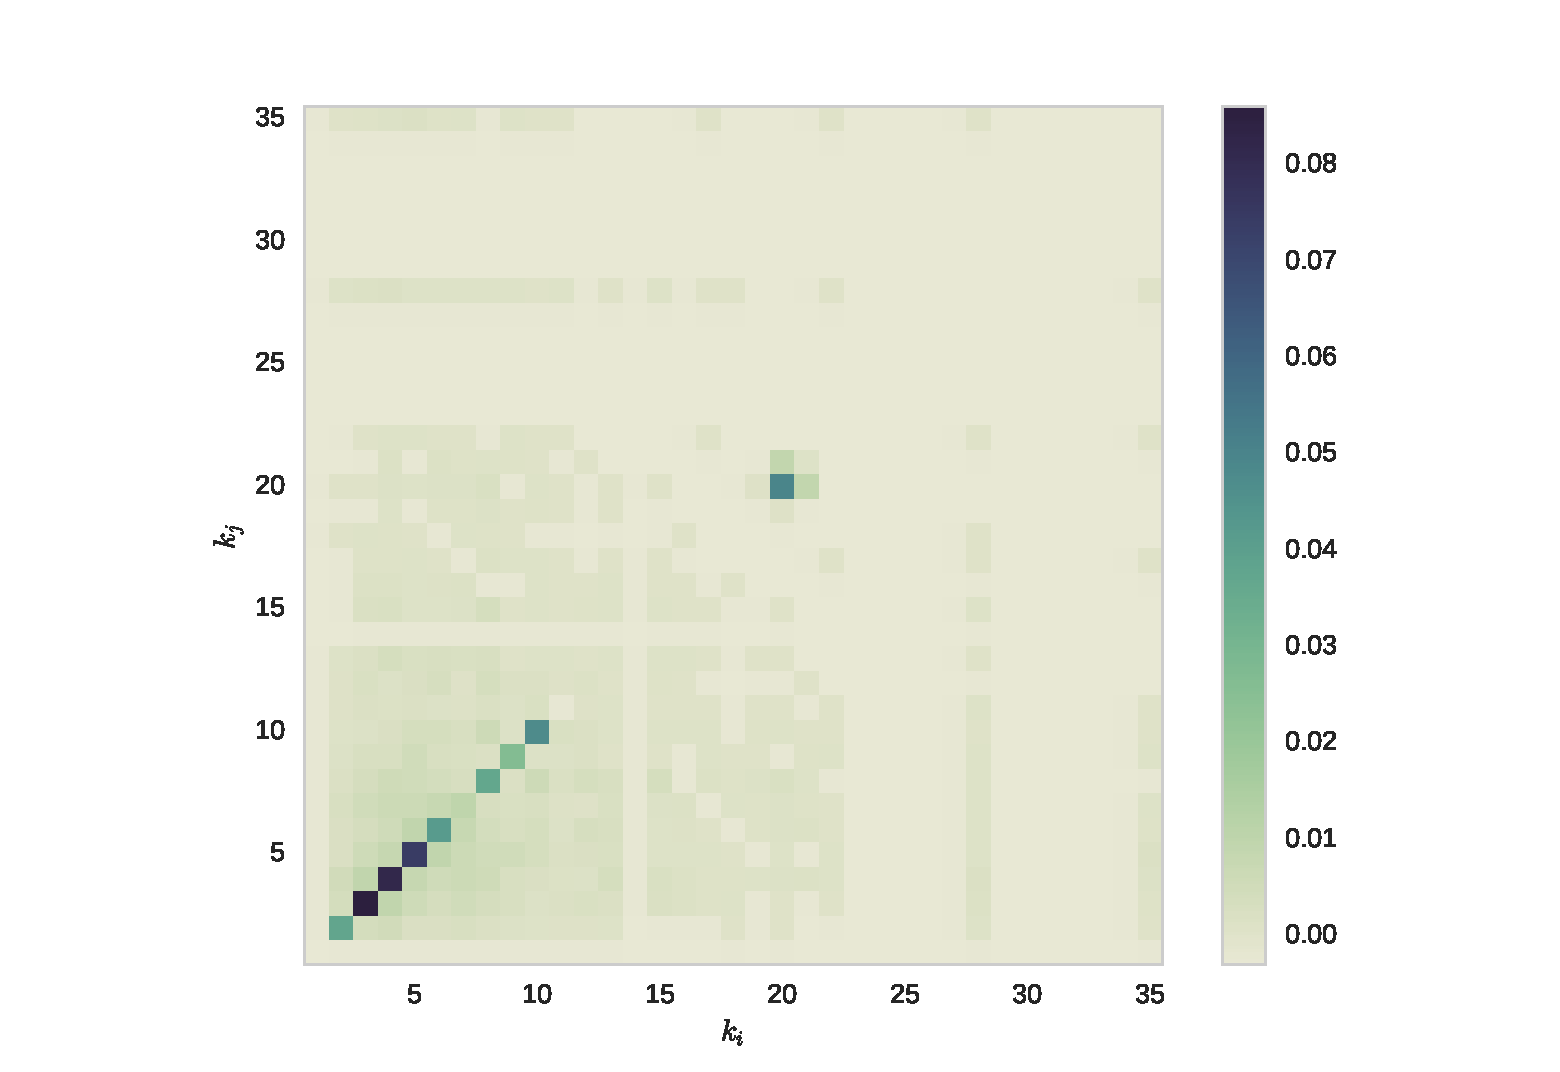
\includegraphics[width=\textwidth]{./schemes/mixing_netscience-gml.pdf}
        \caption{\label{fig4:NETSCIENCE}NETSCIENCE}
    \end{subfigure}
    \begin{subfigure}[b]{0.45\columnwidth}
        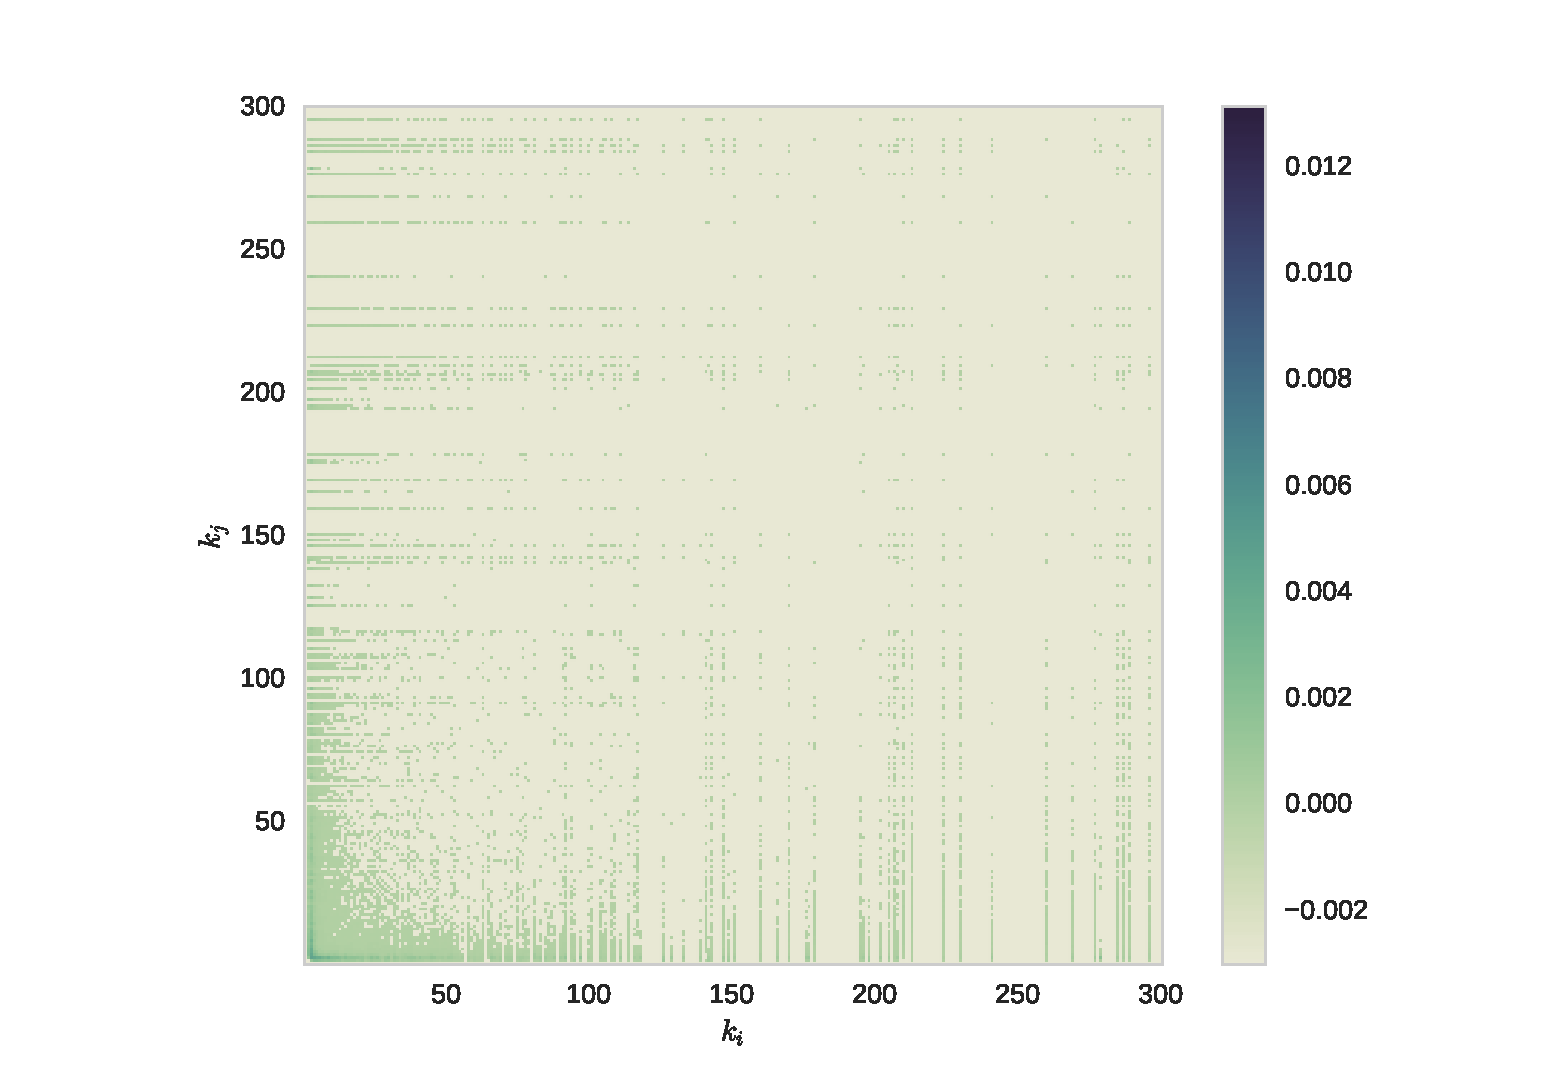
\includegraphics[width=\textwidth]{./schemes/mixing_as-22july06-gml.pdf}
        \caption{\label{fig4:INTERNET}INTERNET}
    \end{subfigure}
    \\
    \begin{subfigure}[b]{0.45\columnwidth}
        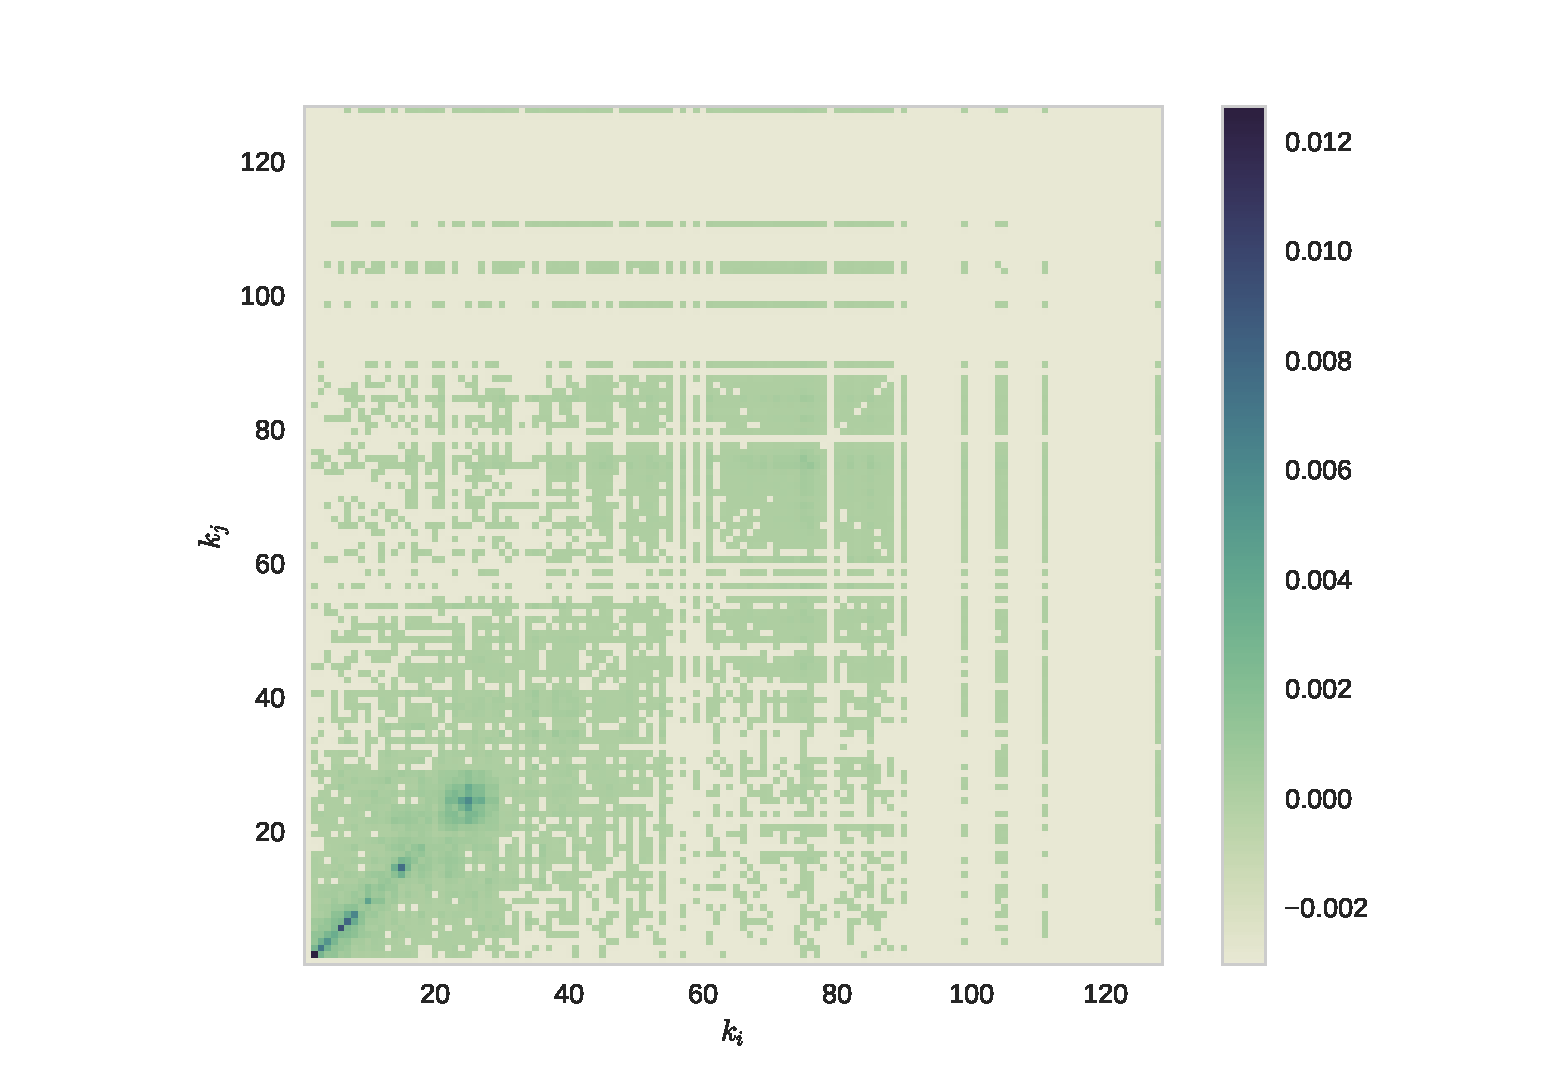
\includegraphics[width=\textwidth]{./schemes/mixing_yeast_AP-MS-txt.pdf}
        \caption{\label{fig4:ap_ms} AP-MS}
    \end{subfigure}
    \begin{subfigure}[b]{0.45\columnwidth}
        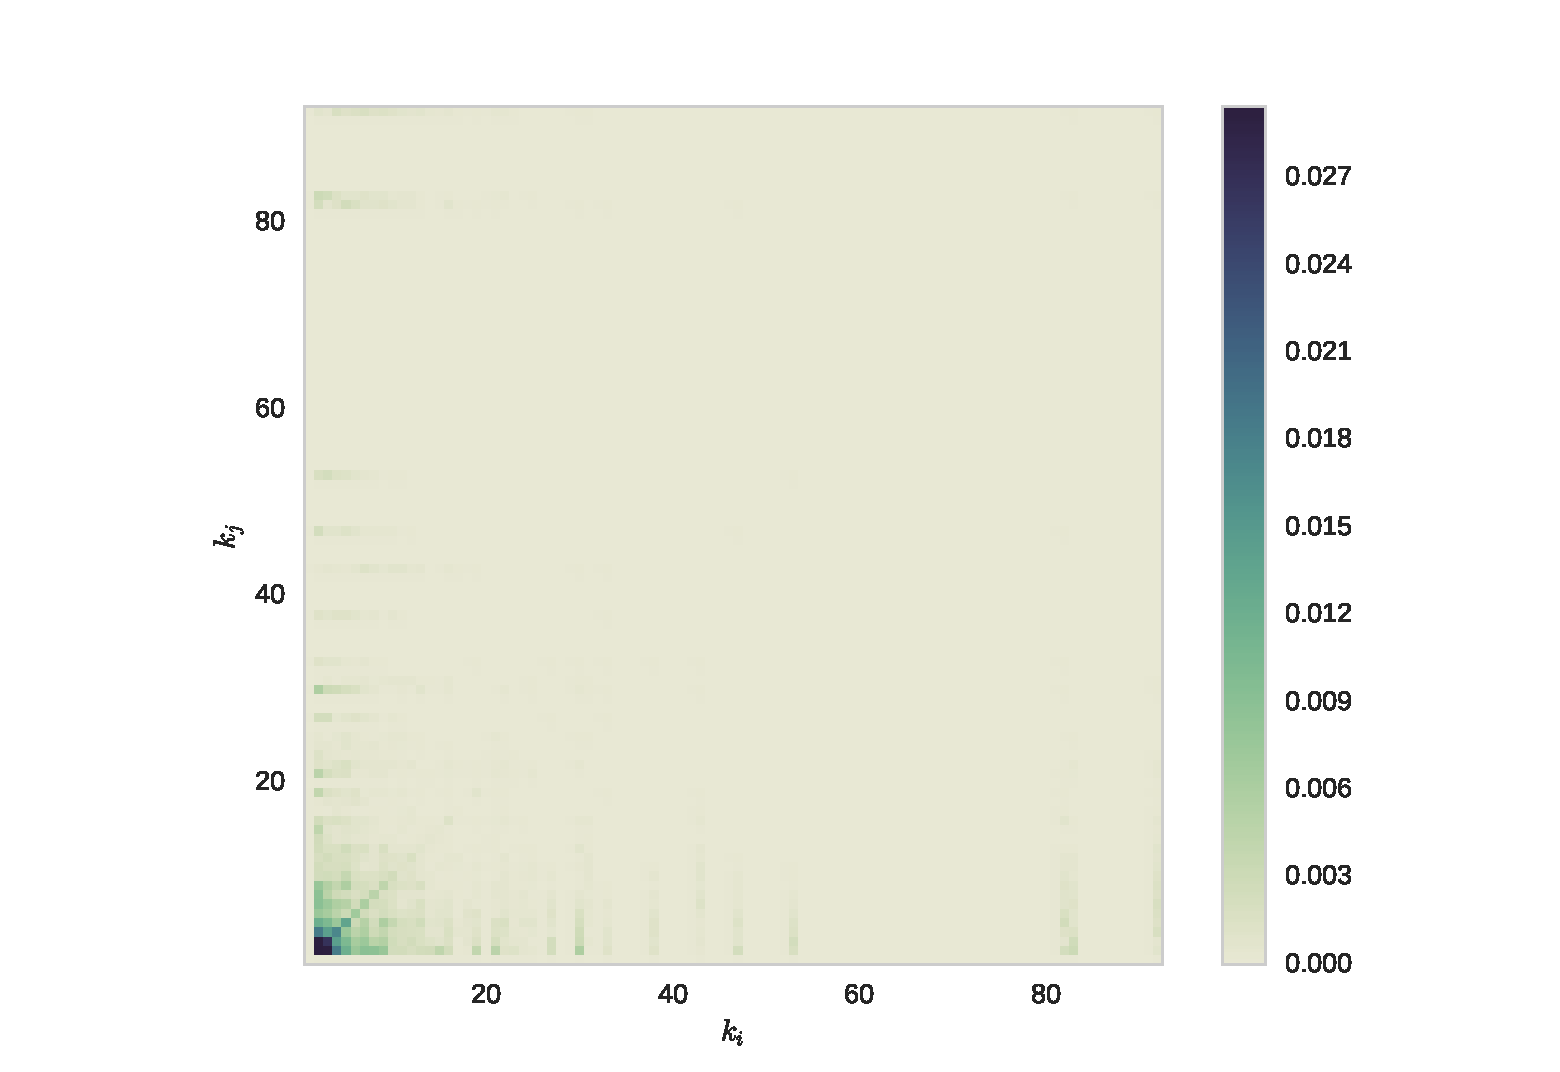
\includegraphics[width=\textwidth]{./schemes/mixing_yeast_Y2H-txt.pdf}
        \caption{\label{fig4:y2h} Y2H}
    \end{subfigure}
    \caption{\label{fig4:mix} Mixing Matrix para cada caso. En la red INTERNET se ha ajustado los limites de gr\'afico
    de manera que sean visibles las correlaciones de bajo grado
    \\(script \texttt{degree\_mixing\_plot.py <archivo>\quad-f <fmt>})}
\end{figure}

De la figura se puede observar que, para todos los casos, la mayor densidad de correlaci\'on se puede encontrar en los 
grados peque\~nos, y para NETSCIENCE y AP-MS parece seguir un comportamiento lineal (\textit{hubs} conectados 
con \textit{hubs}), mientras que en las redes INTERNET y Y2H se puede observar que los nodos de alto grado tienden a 
conectarse con nodos de bajo grado. Sin embargo no es posible tener m\'as que un valor estimativo de la asortividad
con este m\'etodo visual. Es necesario evaluar otras metodolog\'ia.



\subsection{Grado medio del vecindario $k_{nn}$ (revising \citet{barabasi})}
En esta metodolog\'ia estamos interesados en analizar el comportamiento de los vecinos de un nodo de grado $k$, para
ello consideramos el grado medio de los vecinos $k_{nn}$ de un nodo de grado $k$, esto es
\begin{align*}
    k_{nn}(k) = \sum_{k'} k' P(k'|k)
\end{align*}
este promedio est\'a hecho sobre la probabilidad de que: dado un nodo de grado $k$, tenga un vecino de grado $k'$.
Para el caso de una red neutra, en que no existe correlacion entre $k$ y $k'$ ($\text{cov}\left(k,k'\right)=0$) se tiene que
\begin{align*}
    P(k'|k) = P(k') \equiv q_{k'},
\end{align*}
luego 
\begin{align*}
    k_{nn}(k) &= \sum_{k'} k' q_{k'}
\end{align*}
El modelo de Barab\'asi-Albert propone que est\'a probabilidad es $q_{k'} = \frac{k' p_k'}{\mean{k}}$, la probabilidad de 
encontrar un nodo de grado $k'$ al seleccionar un link aleatoreo. As\'i, para el caso neutro
\begin{align*}
    k_{nn}(k) = \frac{\mean{k^2}}{\mean{k}},
\end{align*}
es decir, es constante e independiente de $k$.
Para el caso general, basandose en datos reales, se plantea el modelo 
\begin{align}
    k_{nn}(k) \sim k^\mu.
    \label{knn}
\end{align}

A continuaci\'on se aplica el modelo power law a las redes mostradas en la figura \ref{fig4:grafos} (ver figura \ref{fig4:mu}).
 Aqu\'i se pueden observar los comportamientos asortativos (NETSCIENCE y AP-MS) y disortativos (INTERNET y Y2H).

\begin{figure}[!ht]
    \centering
    \begin{subfigure}[b]{0.45\columnwidth}
        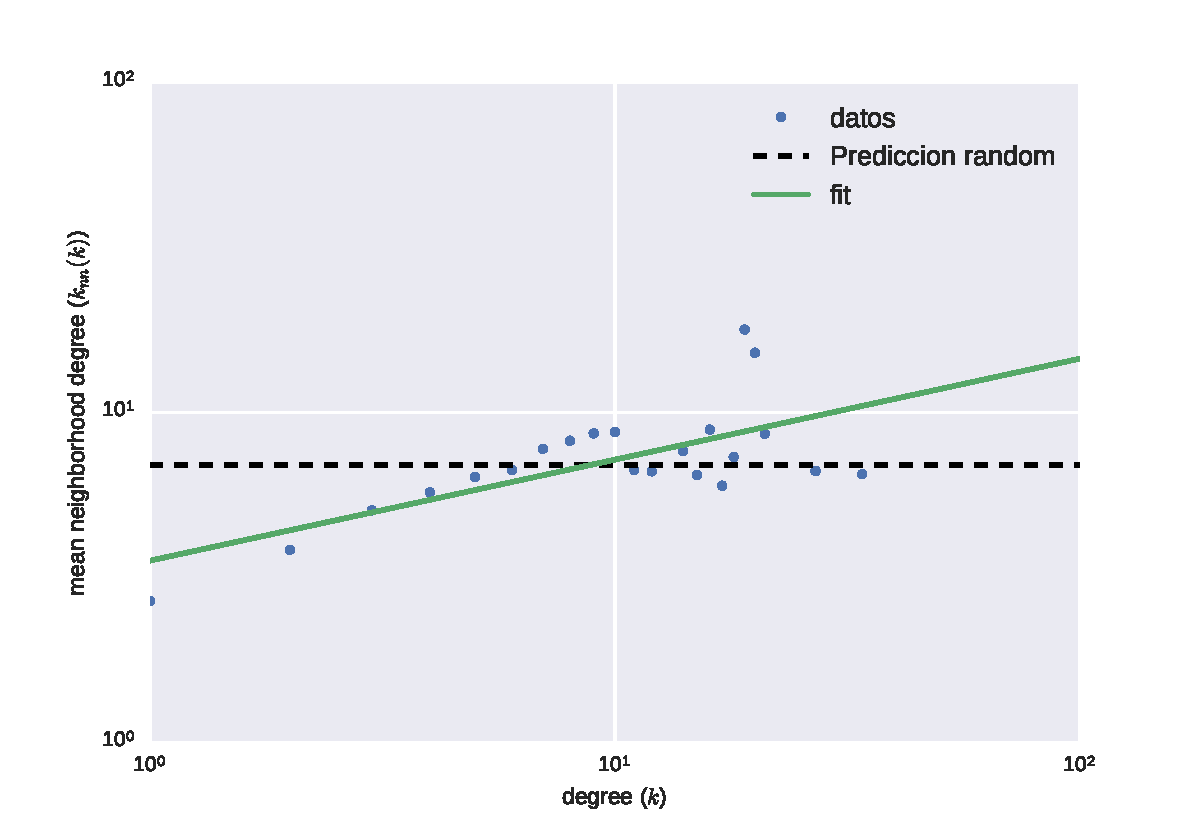
\includegraphics[width=\textwidth]{./schemes/assort_netscience-gml_loglog.pdf}
        \caption{\label{fig4:NETSCIENCE}NETSCIENCE}
    \end{subfigure}
    \begin{subfigure}[b]{0.45\columnwidth}
        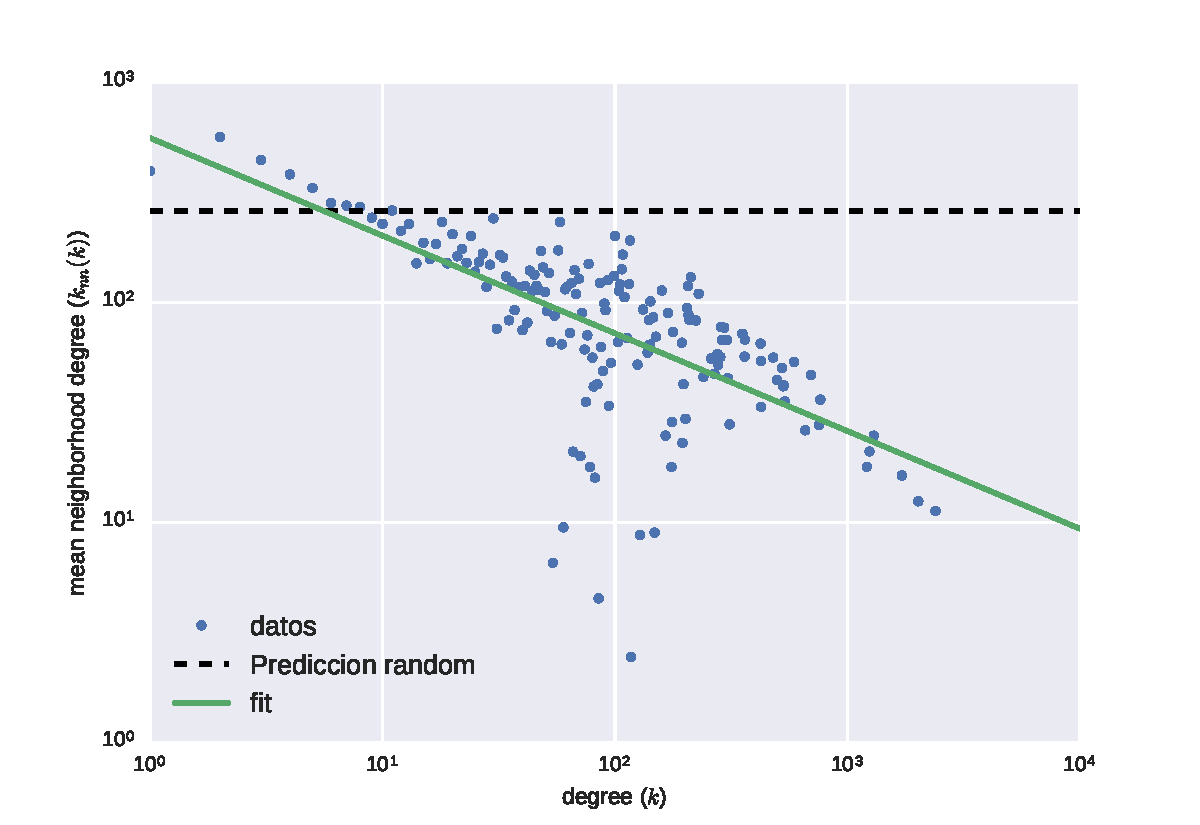
\includegraphics[width=\textwidth]{./schemes/assort_as-22july06-gml_loglog.pdf}
        \caption{\label{fig4:INTERNET}INTERNET}
    \end{subfigure}
    \\
    \begin{subfigure}[b]{0.45\columnwidth}
        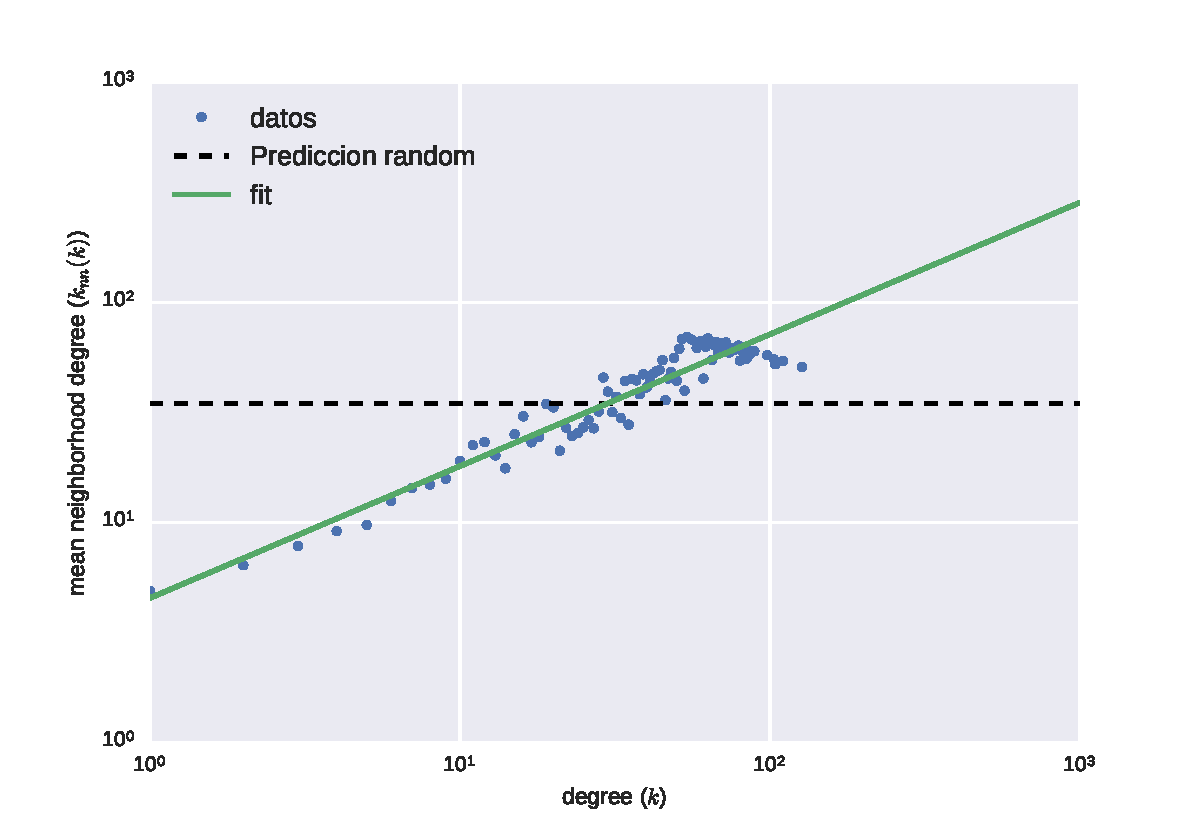
\includegraphics[width=\textwidth]{./schemes/assort_yeast_AP-MS-txt_loglog.pdf}
        \caption{\label{fig4:ap_ms} AP-MS}
    \end{subfigure}
    \begin{subfigure}[b]{0.45\columnwidth}
        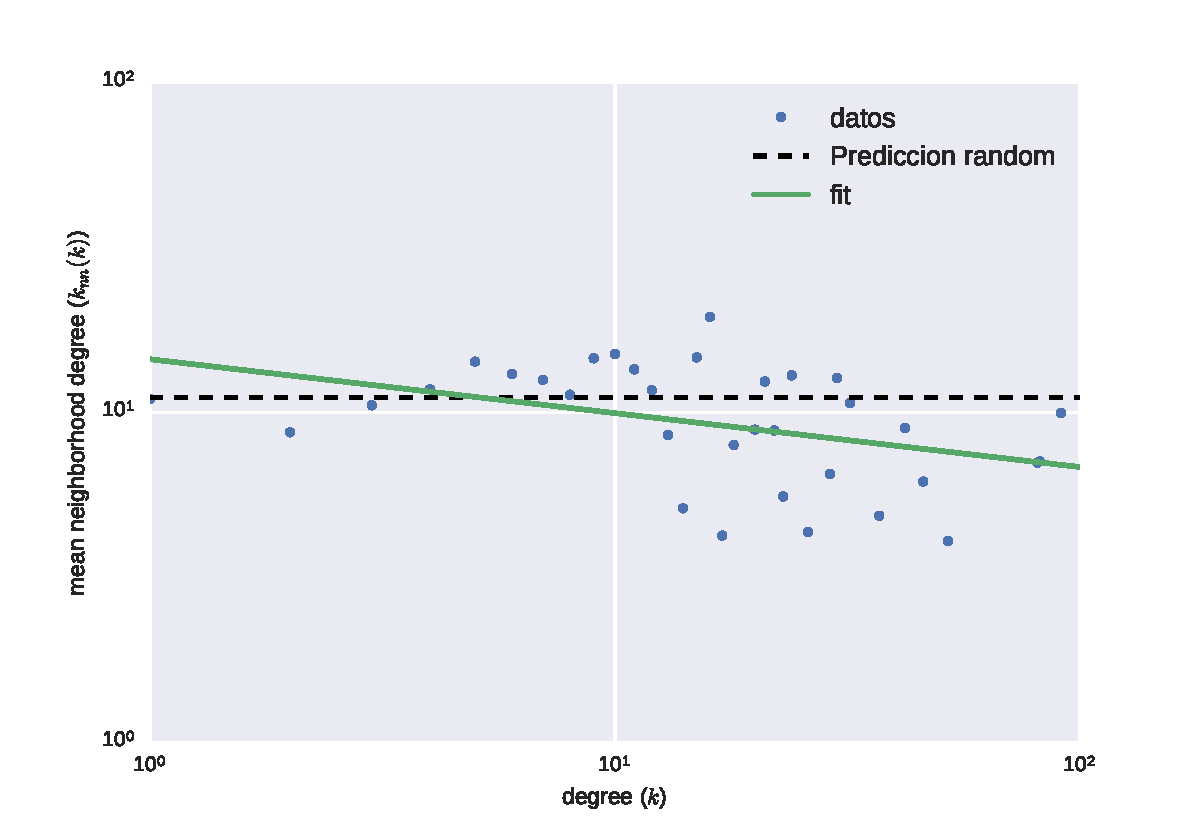
\includegraphics[width=\textwidth]{./schemes/assort_yeast_Y2H-txt_loglog.pdf}
        \caption{\label{fig4:y2h} Y2H}
    \end{subfigure}
    \caption{\label{fig4:mu} Grado medio del vecindario de $k$ para cada red en escala log-log. 
    Fiteo power law (Eq.~\ref{knn}) para cada caso: 
    (a) $\mu \approx 0.306 \pm 0.071$,
    (b) $\mu \approx -0.444 \pm 0.040$,
    (c) $\mu \approx 0.599 \pm 0.019$,
    (d) $\mu \approx -0.163 \pm 0.064$\\
    (script \texttt{assortivity\_powerlaw.py~<archivo>\quad-f <fmt>\quad-l}).}
\end{figure}



\subsection{Coeficiente de Correlaci\'on de Grado}
Por otro lado \citet{newman,newman2003} propuso un coeficiente de correlaci\'on de caracteristica $x$ (tambien llamado 
\textit{coeficiente de asortividad} ) dado por
\begin{align}
    r = \frac{\sum_{ij} \left( A_{ij} - k_i k_j/2m\right) x_i x_j}{\sum_{ij}k_i \delta_{ij} - k_i k_j/2m)x_i x_j}
    \label{r_general}
\end{align}
donde $x$ es la caracteristica una caracter\'istica del nodo, $A$ la matriz de adyacencia, $m$ el n\'umero total de links y $k_i$ el grado del nodo $i$. En el caso particular en que la caracteristica de interes es el grado del nodo, 
entonces la Ec. \ref{r_general} es

\begin{align}
    r = \frac{\sum_{ij} \left( A_{ij} - k_i k_j/2m\right) k_i k_j}{\sum_{ij}(k_i \delta_{ij} - k_i k_j/2m)k_i k_j}
    \label{r_k}
\end{align}

Cabe notar que en \citet{newman} se recomienda implementar de manera distinta para evitar exceso de computos n\'umericos. As\'i, 
tomando $  S_e = \sum_{ij} A_{ij} k_i k_j = 2\sum_{\text{links}(i,j)} k_i k_j $, 
$ S_1 = \sum_i k_i $, $ S_2 = \sum_i k_i^2 $ y $ S_3 = \sum_i k_i^3 $, y reemplazando en Ec.~\ref{r_k}

\begin{align}
    r &= \frac{S_1S_e - S_2^2}{S_1S_3 - S_2^2}
\end{align}

Una implementaci\'on del algoritmo descrito se puede encontrar en \texttt{assortative\_newman.py}. 

\subsection{Discusi\'on}

Para las redes estudiadas, la Tabla \ref{tab:assort} resume los resultados obtenidos 

\begin{table}[!ht]
    \centering
    \caption{\label{tab:assort} Tabla resumen de la asortatividad de las cuatro redes estudiadas.}
    {\scriptsize
    \begin{tabularx}{1\columnwidth}{XlX|XcXcXcX}
        \hline\hline
        & \multirow{2}{*}{Red}  &&& Tipo de     && \multirow{2}{*}{$\mu$}   && \multirow{2}{*}{$r$} &\\ 
        &                       &&& Asortividad &&                          &&                      &\\ 
        \hline
        & NETSCIENCE           &&& Asortativa   &&   0.306                  &&  0.461                &\\
        & INTERNET             &&& Disortativa  &&  -0.444                  && -0.198                &\\
        & AP-MS                &&& Asortativa   &&   0.599                  &&  0.461                &\\
        & Y2H                  &&& Disortativa  &&  -0.163                  && -0.041                &\\
        \hline\hline
    \end{tabularx}
    }
\end{table}

\citet{newman2003} reporta las asortatividad de 27 redes y obtiene que ciertos rangos de asortividad son caracteristicos del 
tipo de red en cuesti\'on, por ejemplo, por un lado redes biol\'ogicas suelen ser disortativas y por otro las redes sociales
tienen un comportamiento asortativo. En particular, en internet los  servidores (\textit{hubs}) no suelen conectarse 
entre ellos si no que m\'as bien reciben un gigantesco n\'umero de usuarios (nodos) y servidores peque\~nos, lo que explica
el comportamiento disortativo. Por otro lado, la red AP-MS est\'a construida a partir de medici\'on de afinidad, generando
grandes clusters altamente conectados entre ellos, est\'a manera de construir la red es probable que este asociada con la 
asortatividad reportada. Sin embargo, es necesario analizar rigurosamente tipo de asortatividad/disotatividad de estas redes
(si son disortatividades estructurales o no). Los ultimos dos casos (NETSCIENCE y Y2H) responden a los comportamientos
usuales para sus categor\'ias (redes sociales y biol\'ogicas respectivamente).




\end{document}
